% Options for packages loaded elsewhere
\PassOptionsToPackage{unicode}{hyperref}
\PassOptionsToPackage{hyphens}{url}
%
\documentclass[
]{book}
\usepackage{amsmath,amssymb}
\usepackage{iftex}
\ifPDFTeX
  \usepackage[T1]{fontenc}
  \usepackage[utf8]{inputenc}
  \usepackage{textcomp} % provide euro and other symbols
\else % if luatex or xetex
  \usepackage{unicode-math} % this also loads fontspec
  \defaultfontfeatures{Scale=MatchLowercase}
  \defaultfontfeatures[\rmfamily]{Ligatures=TeX,Scale=1}
\fi
\usepackage{lmodern}
\ifPDFTeX\else
  % xetex/luatex font selection
\fi
% Use upquote if available, for straight quotes in verbatim environments
\IfFileExists{upquote.sty}{\usepackage{upquote}}{}
\IfFileExists{microtype.sty}{% use microtype if available
  \usepackage[]{microtype}
  \UseMicrotypeSet[protrusion]{basicmath} % disable protrusion for tt fonts
}{}
\makeatletter
\@ifundefined{KOMAClassName}{% if non-KOMA class
  \IfFileExists{parskip.sty}{%
    \usepackage{parskip}
  }{% else
    \setlength{\parindent}{0pt}
    \setlength{\parskip}{6pt plus 2pt minus 1pt}}
}{% if KOMA class
  \KOMAoptions{parskip=half}}
\makeatother
\usepackage{xcolor}
\usepackage{longtable,booktabs,array}
\usepackage{calc} % for calculating minipage widths
% Correct order of tables after \paragraph or \subparagraph
\usepackage{etoolbox}
\makeatletter
\patchcmd\longtable{\par}{\if@noskipsec\mbox{}\fi\par}{}{}
\makeatother
% Allow footnotes in longtable head/foot
\IfFileExists{footnotehyper.sty}{\usepackage{footnotehyper}}{\usepackage{footnote}}
\makesavenoteenv{longtable}
\usepackage{graphicx}
\makeatletter
\def\maxwidth{\ifdim\Gin@nat@width>\linewidth\linewidth\else\Gin@nat@width\fi}
\def\maxheight{\ifdim\Gin@nat@height>\textheight\textheight\else\Gin@nat@height\fi}
\makeatother
% Scale images if necessary, so that they will not overflow the page
% margins by default, and it is still possible to overwrite the defaults
% using explicit options in \includegraphics[width, height, ...]{}
\setkeys{Gin}{width=\maxwidth,height=\maxheight,keepaspectratio}
% Set default figure placement to htbp
\makeatletter
\def\fps@figure{htbp}
\makeatother
\setlength{\emergencystretch}{3em} % prevent overfull lines
\providecommand{\tightlist}{%
  \setlength{\itemsep}{0pt}\setlength{\parskip}{0pt}}
\setcounter{secnumdepth}{5}
\usepackage{booktabs}
\ifLuaTeX
  \usepackage{selnolig}  % disable illegal ligatures
\fi
\usepackage[]{natbib}
\bibliographystyle{plainnat}
\IfFileExists{bookmark.sty}{\usepackage{bookmark}}{\usepackage{hyperref}}
\IfFileExists{xurl.sty}{\usepackage{xurl}}{} % add URL line breaks if available
\urlstyle{same}
\hypersetup{
  pdftitle={Topology},
  pdfauthor={Ashan Jayamal},
  hidelinks,
  pdfcreator={LaTeX via pandoc}}

\title{Topology}
\author{Ashan Jayamal}
\date{2024-03-23}

\usepackage{amsthm}
\newtheorem{theorem}{Theorem}[chapter]
\newtheorem{lemma}{Lemma}[chapter]
\newtheorem{corollary}{Corollary}[chapter]
\newtheorem{proposition}{Proposition}[chapter]
\newtheorem{conjecture}{Conjecture}[chapter]
\theoremstyle{definition}
\newtheorem{definition}{Definition}[chapter]
\theoremstyle{definition}
\newtheorem{example}{Example}[chapter]
\theoremstyle{definition}
\newtheorem{exercise}{Exercise}[chapter]
\theoremstyle{definition}
\newtheorem{hypothesis}{Hypothesis}[chapter]
\theoremstyle{remark}
\newtheorem*{remark}{Remark}
\newtheorem*{solution}{Solution}
\begin{document}
\maketitle

{
\setcounter{tocdepth}{1}
\tableofcontents
}
\hypertarget{topology}{%
\chapter{Topology}\label{topology}}

A topology is a geometric structure defined on a set. Basically it is given by declaring which subsets are ``open'' sets. Thus the axioms are the abstraction of the properties that open sets have.

\hypertarget{topological-spaces}{%
\section{Topological Spaces}\label{topological-spaces}}

\begin{definition}
\protect\hypertarget{def:Top}{}\label{def:Top}A topology on a set \(X\) is a collection \(\mathcal{T}\) of subsets of \(X\) such that

(T1) \(\phi\) and \(X\) are in \(\mathcal{T}\);

(T2) Any union of subsets in \(\mathcal{T}\) is in \(\mathcal{T}\);

(T3) The finite intersection of subsets in \(\mathcal{T}\) is in \(\mathcal{T}\).
\end{definition}

A set \(X\) with a topology \(\mathcal{T}\) is called a topological space. Denoted by \((X,\mathcal{T})\). An element of \(\mathcal{T}\) is called an open set.

\begin{example}
\protect\hypertarget{exm:unnamed-chunk-1}{}\label{exm:unnamed-chunk-1}Let \(X\) be a three-element set, \(X = \{a, b, c\}\) and \(\mathcal{T}=\{X, \emptyset,\{a, b\}, \{b\}, \{b, c\}\}\). We can check T1,T2 and T3 conditions.
\end{example}

\begin{example}
\protect\hypertarget{exm:unnamed-chunk-2}{}\label{exm:unnamed-chunk-2}Let \(X\) be a three-element set, \(X = \{a, b, c\}\) as pervoius. There are many possible topologies on \(X\), some of which are indicated schematically in figure \ref{fig:gi}. Furthur, we can see that even a three-element set has many different topologies.
\end{example}

\begin{figure}
\centering
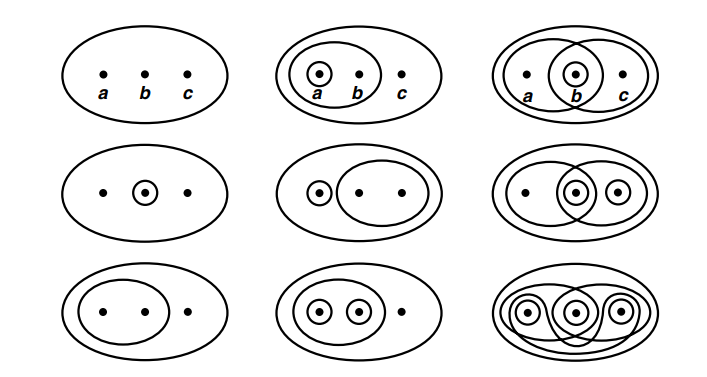
\includegraphics{figures/figure 01.png}
\caption{\label{fig:gi}\(~\)}
\end{figure}

\begin{remark}
Not every collection of subsets of \(X\) is a topology on \(X\). Observe that Neither of the collections indicated in figure \ref{fig:fig2} is a topology.

First let's consider the left hand coner of figure \ref{fig:fig2}. \(\{a\}\) and \(\{b\}\) in the collection, but \(\{a\}\cup \{b\}\) is not in the collection.

Now consider the right hand coner figure. \(\{a,b\}\) and \(\{b,c\}\) in collection, but \(\{a,b\}\cap\{b,c\}=\{b\}\) is not in the collection.
\end{remark}

\begin{figure}
\centering
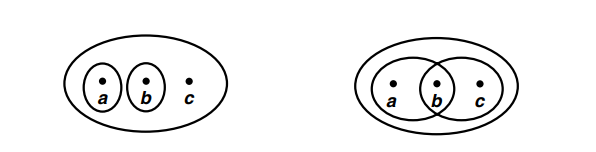
\includegraphics{figures/figure 02.png}
\caption{\label{fig:fig2}\(~\)}
\end{figure}

\begin{example}
\protect\hypertarget{exm:unnamed-chunk-4}{}\label{exm:unnamed-chunk-4}If \(X\) is any set, the collection of all subsets of \(X\) (Power set) is a topology on \(X\). This trivail statified T1 T2 and T3 conditions. Furthur,This is called the \emph{discrete topology}.
\end{example}

\begin{example}
\protect\hypertarget{exm:unnamed-chunk-5}{}\label{exm:unnamed-chunk-5}The collection consisting of \(X\) and \(\emptyset\) only is also a topologyon \(X\). we shall call it the \emph{indiscrete topology}, or the trivial topology.
\end{example}

\begin{example}
\protect\hypertarget{exm:unnamed-chunk-6}{}\label{exm:unnamed-chunk-6}Let \(X\) be a set and let \(\mathcal{T}_f\) be the collection of all subsets U of X such that \(X\setminus U\) either is finite or is all of \(X\). In oter words,
\[\mathcal{T}_f:=\left\{U\subseteq X : \text{Either is finite or is all of } X\right\}\]
Let's check is \(\mathcal{T}_f\) a topology. First obseve that both \(X\) and \(\emptyset\) are in \(\mathcal{T}_f\) , because \(X\setminus X=\emptyset\) is finite and \$X\setminus \emptyset \$ is all of \(X\).So \(\mathcal{T}_f\) statified the T1 condition. Now let's check the T2 condition. Let \(\{U_{\alpha}:\alpha\in I, I \text{ is index set}\}\).Now we need to show that \(\cup{\alpha\in I} U_\alpha\in \mathcal{T}_f\). So consider,
\[X\setminus \bigcup_{\alpha\in I} U_\alpha =\bigcap_{\alpha\in I} (X\setminus  U_\alpha).\]
Now obsevere that \(\cap_{\alpha\in I} (X\setminus U_\alpha)\) is finite, because each set \((X\setminus U_\alpha)\) is finite and arbitary intersection of finite sets is finite. So, \(\mathcal{T}_f\) stattified the T2 condition also.
Finaly check the last condition, T3 condition. Let \(U_1,...,U_n\) are nonempty elements of \(\mathcal{T}_f\) , to show that \(\bigcup_i U_i \in \mathcal{T}_f\) , we compute
\[X\setminus \bigcap_{i=1}^n U_i = \bigcup_{i=1}^n(X \setminus U_i).\]
Note that the set \(\bigcup_{i=1}^n(X \setminus U_i)\) is a finite union of finite sets and, therefore, finite. So it statisfiy the T3 condition also. Thefore \(\mathcal{T}_f\) is a topology. Furthur \(\mathcal{T}_f\) is called the finite \emph{complement topology}.
\end{example}

\begin{example}
\protect\hypertarget{exm:unnamed-chunk-7}{}\label{exm:unnamed-chunk-7}Let \(X\) be a set. Define \(\mathcal{T}\) to be the collection of all subsets \(U\) of \(X\) such that \(X\setminus U\) either is finite or is all of \(X\). Then \(\mathcal{T}\) defines a topology on \(X\), called finite complement topology of \(X\).
\end{example}

\hypertarget{basis-of-a-topology}{%
\section{Basis of a Topology}\label{basis-of-a-topology}}

Once we define a structure on a set, often we try to understand what the minimum data you need to specify the structure. In many cases, this minimum data is called a basis and we say that the basis generate the structure. The notion of a basis of the structure will help us to describe examples more systematically.

\begin{definition}
\protect\hypertarget{def:unnamed-chunk-8}{}\label{def:unnamed-chunk-8}Let \(X\) be a set. A basis of a topology on \(X\) is a collection \(\mathcal{B}\) of subsets in \(X\) such that

(B1) For every \(x \in X\), there exist an element \(B\) in \(\mathcal{B}\) such that \(x \in B\).

(B2) If \(x \in B_{1} \cap B_{2}\) where \(B_{1}, B_{2}\) are in \(\mathcal{B}\), then there is \(B_{3}\) in \(\mathcal{B}\) such that \(x \in B_{3} \subseteq B_{1} \cap B_{2}\).
\end{definition}

\begin{figure}
\centering
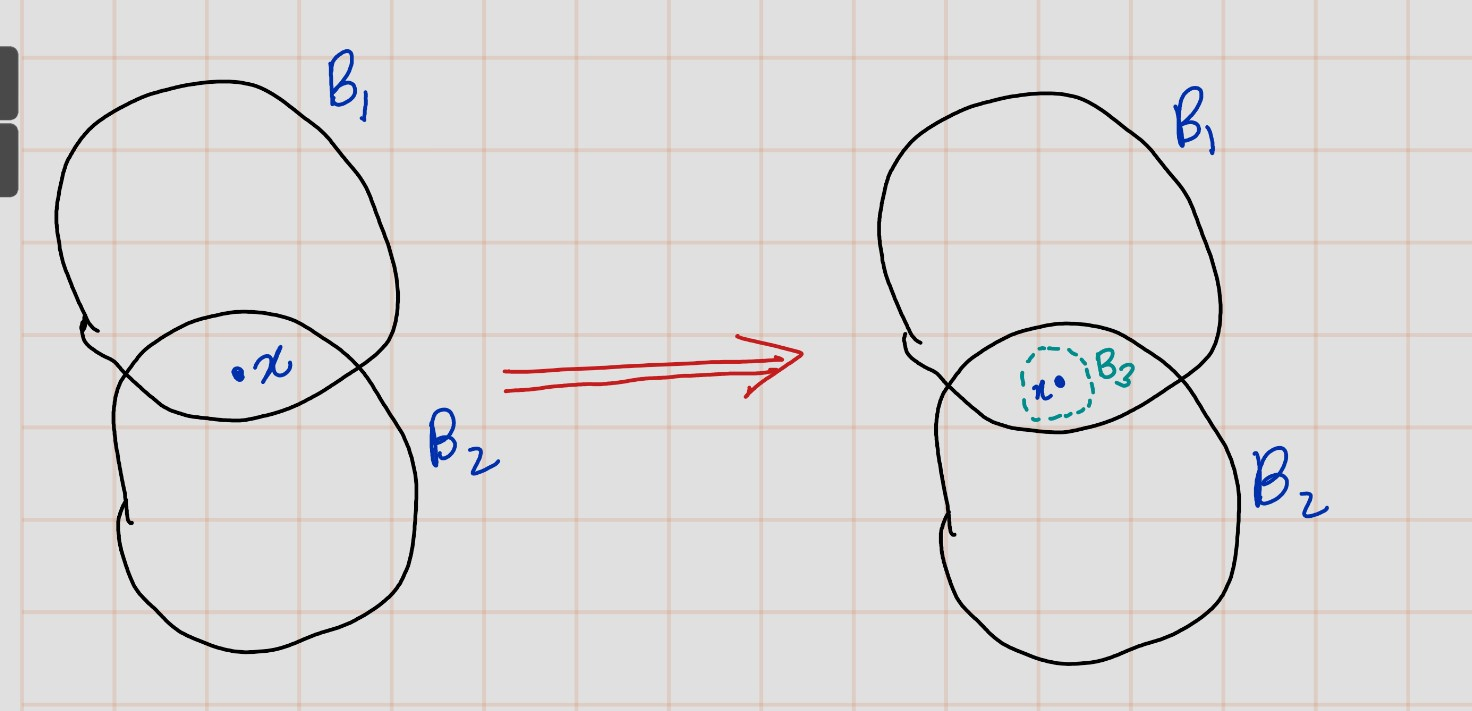
\includegraphics{figures/figure 03.jpg}
\caption{\label{fig:fig3}\(~\)}
\end{figure}

\begin{lemma}[Generating of a topology]
\protect\hypertarget{lem:unnamed-chunk-9}{}\label{lem:unnamed-chunk-9}Let \(\mathcal{B}\) be a basis of a topology on X. Define \(\mathcal{T}_{\mathcal{B}}\) to be the collection of subsets \(U \subset X\) satisfting

(G1) For every \(x \in U\), there is \(B \in \mathcal{B}\) such that \(x \in B \subset U\).

Then \(\mathcal{T}_{\mathcal{B}}\) defines a topology on \(X\). Here we assume that \(\emptyset\) trivially satisfies the condition, so that \(\emptyset \in \mathcal{T}_{\mathcal{B}}\).
\end{lemma}

\begin{proof}

We need to check the three axioms:

\begin{itemize}
\item
  (T1) \(\emptyset \in \mathcal{T}_{\mathcal{B}}\) as we assumed. \(X \in \mathcal{T}_{\mathcal{B}}\) by (B1).
\item
  (T2) Consider a collection of subsets \(U_{\alpha} \in \mathcal{T}_{\mathcal{B}}, \alpha \in \mathrm{J}\). We need to show
\end{itemize}

\[
U:=\bigcup_{\alpha \in J} U_{\alpha} \quad \in \mathcal{T}_{\mathcal{B}}
\]
By the definition of the union, for each \(x \in U\), there is \(U_{\alpha}\) such that \(x \in U_{\alpha}\). Since \(U_{\alpha} \in \mathcal{T}_{\mathcal{B}}\), there is \(B \in \mathcal{B}\) such that \(x \in B \subset U_{\alpha}\). Since \(U_{\alpha} \subset U\), we found \(B \in \mathcal{B}\) such that \(x \in B \subset U\). Thus \(U \in \mathcal{T}_{\mathcal{B}}\).

\begin{itemize}
\item
  (T3) Now consider a finite number of subsets \(U_{1},..., U_{n} \in \mathcal{T}_{\mathcal{B}}\). We need to show that
  \[
  U':=\bigcap_{i=1}^{n} U_{i} \quad \in \mathcal{T}_{\mathcal{B}}
  \]
\item
  Let's just check for two subsets \(U_{1}, U_{2}\) first. For each \(x \in U_{1} \cap U_{2}\), there are \(B_{1}, B_{2} \in \mathcal{B}\) such that \(x \in B_{1} \subset U_{1}\) and \(x \in B_{2} \subset U_{2}\). This is because \(U_{1}, U_{2} \in \mathcal{T}_{\mathcal{B}}\) and \(x \in U_{1}, x \in U_{2}\). By (B2), there is \(B_{3} \in \mathcal{B}\) such that \(x \in B_{3} \subset B_{1} \cap B_{2}\). Now we found \(B_{3} \in \mathcal{B}\) such that \(x \in B_{3} \subset U\).
\item
  We can generalize the above proof to \(n\) subsets, but let's use induction to prove it. This is going to be the induction on the number of subsets.

  \begin{itemize}
  \tightlist
  \item
    When \(n=1\), the claim is trivial.
  \item
    Suppose that the claim is true when we have \(n-1\) subsets, i.e.~\(U_{1} \cap \cdots \cap U_{n-1} \in \mathcal{T}_{\mathcal{B}}\). Since \[
    U=U_{1} \cap \cdots \cap U_{n}=\left(U_{1} \cap \cdots \cap U_{n-1}\right) \cap U_{n}
    \]
    and regarding \(U^{\prime}:=U_{1} \cap \cdots \cap U_{n-1}\), we have two subsets case \(U=U^{\prime} \cap U_{n}\). By the first arguments, \(U \in \mathcal{T}_{\mathcal{B}}\).
  \end{itemize}
\end{itemize}

\end{proof}

\begin{definition}
\protect\hypertarget{def:unnamed-chunk-11}{}\label{def:unnamed-chunk-11}\(\mathcal{T}_{\mathcal{B}}\) is called the \textbf{topology generated by a basis \(\mathcal{B}\)}. On the other hand, if \((X, \mathcal{T})\) is a topological space and \(\mathcal{B}\) is a basis of a topology such that \(\mathcal{T}_{\mathcal{B}}=\mathcal{T}\), then we say \(\mathcal{B}\) is a basis of \(\mathcal{T}\). Note that \(\mathcal{T}\) itself is a basis of the topology \(\mathcal{T}\). So there is always a basis for a given topology.
\end{definition}

\begin{example}
\protect\hypertarget{exm:unnamed-chunk-12}{}\label{exm:unnamed-chunk-12}\leavevmode

\begin{itemize}
\item
  (Standard Topology of \(\mathbb{R}\) ) Let \(\mathbb{R}\) be the set of all real numbers. Let \(\mathcal{B}\) be the collection of all open intervals:
  \[
  (a, b):=\{x \in \mathbb{R} \mid a<x<b\}
  \]
  Then \(\mathcal{B}\) is a basis of a topology and the topology generated by \(\mathcal{B}\) is called the standard topology of \(\mathbb{R}\).
\item
  Let \(\mathbb{R}^{2}\) be the set of all ordered pairs of real numbers, i.e.~\(\mathbb{R}^{2}:=\mathbb{R} \times \mathbb{R}\) (cartesian product). Let \(\mathcal{B}\) be the collection of cartesian product of open intervals, \((a, b) \times(c, d)\). Then \(\mathcal{B}\) is a basis of a topology and the topology generated by \(\mathcal{B}\) is called the standard topology of \(\mathbb{R}^{2}\).
\item
  (Lower limit topology of \(\mathbb{R}\) ) Consider the collection \(\mathcal{B}\) of subsets in \(\mathbb{R}\) :
  \[
  \mathcal{B}:=\{[a, b):=\{x \in \mathbb{R} \mid a \leq x<b\} \mid a, b \in \mathbb{R}\}
  \]
  This is a basis for a topology on \(\mathbb{R}\). This topology is called the lower limit topology.
\end{itemize}

\end{example}

The following two lemma are useful to determine whehter a collection \(\mathcal{B}\) of open sets in \(\mathcal{T}\) is a basis for \(\mathcal{T}\) or not.

\begin{remark}
Let \(\mathcal{T}\) be a topology on \(X\). If \(\mathcal{B} \subset \mathcal{T}\) and \(\mathcal{B}\) satisfies (B1) and (B2), it is easy to see that \(\mathcal{T}_{\mathcal{B}} \subset \mathcal{T}\). This is just because of (G1). If \(U \in \mathcal{T}_{\mathcal{B}}\), (G1) is satisfied for \(U\) so that \(\forall x \in U, \exists B_{x} \in \mathcal{B}\) such that \(x \in B_{x} \subset U\). Therefore \(U=\cup_{x \in U} B_{x}\). By (T2), \(U \in \mathcal{T}\).
\end{remark}

\begin{lemma}
\protect\hypertarget{lem:lemmaTequalsTB}{}\label{lem:lemmaTequalsTB}Let \((X, \mathcal{T})\) be a topological space. Let \(\mathcal{B} \subset \mathcal{T}\). Then \(\mathcal{B}\) is a basis and \(\mathcal{T}_{\mathcal{B}}=\mathcal{T}\) if and only if \(\mathcal{T}\) is the set of all unions of elements in \(\mathcal{B}\).
\end{lemma}

\begin{proof}
\leavevmode

\begin{itemize}
\tightlist
\item
  \(\quad(\Rightarrow)\) Let \(\mathcal{T}^{\prime}\) be the set of all unions of open sets in \(\mathcal{B}\). If \(U \in \mathcal{T}\), then \(U\) satisfies (G1), i.e.~\(\forall x \in U, \exists B_{x} \in \mathcal{B}\) s.t. \(x \in B_{x} \subset U\). Thus \(U=\cup_{x \in U} B_{x}\). Therefore \(U \in \mathcal{T}^{\prime}\). We proved \(\mathcal{T} \subset \mathcal{T}^{\prime}\). It follows from (T2) that \(\mathcal{T}^{\prime} \subset \mathcal{T}\).
\item
  \((\Leftarrow)\) Since \(X \in \mathcal{T}, X=\cup_{\alpha} B_{\alpha}\) some union of sets in \(\mathcal{B}\). Thus \(\forall x \in X, \exists B_{\alpha}\) s.t. \(x \in B_{\alpha}\). This proves (B1) for \(\mathcal{B}\). If \(B_{1}, B_{2} \in \mathcal{B}\), then \(B_{1} \cap B_{2} \in \mathcal{T}\) by (T2). Thus \(B_{1} \cap B_{2}=\cup_{\alpha} B_{\alpha}, B_{\alpha} \in \mathcal{B}\). So \(\forall x \in B_{1} \cap B_{2}, \exists B_{\alpha} \in B\) s.t. \(x \in B_{\alpha}\). This \(B_{\alpha}\) plays the role of \(B_{3}\) in (B2). Thus \(\mathcal{B}\) is a basis. Now it makes sense to consider \(\mathcal{T}_{\mathcal{B}}\) and we need to show \(\mathcal{T}_{\mathcal{B}}=\mathcal{T}\). By the remark, we already know that \(\mathcal{T}_{\mathcal{B}} \subset \mathcal{T}\). On the other hand, if \(U \in \mathcal{T}\), then \(U=\cup_{\alpha} B_{\alpha}, B_{\alpha} \in \mathcal{B}\). Hence, \(\forall x \in U, \exists B_{\alpha}\) such that \(x \in B_{\alpha} \subset U\). Thus (G1) is satisfied for \(U\). Thus \(U \in \mathcal{T}_{\mathcal{B}}\). This proves \(\mathcal{T}_{\mathcal{B}} \supset \mathcal{T}\).
\end{itemize}

\end{proof}

\begin{lemma}
\protect\hypertarget{lem:lemma110}{}\label{lem:lemma110}Let \((X, \mathcal{T})\) be a topological space. Let \(\mathcal{B} \subset \mathcal{T}\). Then \(\mathcal{B}\) is a basis and \(\mathcal{T}_{\mathcal{B}}=\mathcal{T}\) if and if any \(U \in \mathcal{T}\) satisfies (Gl), i.e.~\(\forall x \in U, \exists B_{x} \in \mathcal{B}\) s.t. \(x \in B_{x} \subset U\).
\end{lemma}

\begin{proof}
\leavevmode

\begin{itemize}
\item
  (\(\Rightarrow\)) Trivial by the definition of \(\mathcal{T}_{\mathcal{B}}\).
\item
  (\(\Leftarrow X\)) satisfies (G1) so \(\mathcal{B}\) satisfies (B1). Let \(B_{1}, B_{2} \in \mathcal{B} \subset \mathcal{T}\). By (T3), \(B_{1} \cap B_{2} \in \mathcal{T}\). Thus \(B_{1} \cap B_{2}\) satisfies (G1). This means (B2) holds for \(\mathcal{B}\). Thus \(\mathcal{B}\) is a basis. Now the assumption can be rephrased as \(\mathcal{T} \subset \mathcal{T}_{\mathcal{B}}\). By the remark above, we already know \(\mathcal{T} \supset \mathcal{T}_{\mathcal{B}}\).
\end{itemize}

\end{proof}

\hypertarget{comparing-topologies}{%
\section{Comparing Topologies}\label{comparing-topologies}}

\begin{definition}
\protect\hypertarget{def:unnamed-chunk-16}{}\label{def:unnamed-chunk-16}Let \(\mathcal{T}, \mathcal{T}^{\prime}\) be two topologies for a set \(X\). We say \(\mathcal{T}^{\prime}\) is finer than \(\mathcal{T}\) or \(\mathcal{T}\) is coarser than \(\mathcal{T}^{\prime}\) if \(\mathcal{T} \subset \mathcal{T}^{\prime}\). The intuition for this notion is '' \(\left(X, \mathcal{T}^{\prime}\right)\) has more open subsets to separate two points in \(X\) than \((X, \mathcal{T})\) ``.
\end{definition}

\begin{lemma}
\protect\hypertarget{lem:finerLemma}{}\label{lem:finerLemma}Let \(\mathcal{B}, \mathcal{B}^{\prime}\) be bases of topologies \(\mathcal{T}, \mathcal{T}^{\prime}\) on \(X\) respectively. Then \(\mathcal{T}^{\prime}\) is finer than \(\mathcal{T} \Leftrightarrow\) \(\forall B \in \mathcal{B}\) and \(\forall x \in B, \exists B^{\prime} \in \mathcal{B}^{\prime}\) s.t. \(x \in B^{\prime} \subseteq B\).
\end{lemma}

\begin{proof}
\leavevmode

\begin{itemize}
\item
  \(\Rightarrow\) Since \(\mathcal{B} \subset \mathcal{T} \subset \mathcal{T}^{\prime}\), all subsets in \(\mathcal{B}\) satisfies (G1) for \(\mathcal{T}^{\prime}\), which is exactly the statement we wanted to prove.
\item
  \(\Leftarrow\) The LHS says \(\mathcal{B} \subset \mathcal{T}^{\prime}\). We need to show that it implies that any \(U \in \mathcal{T}\) satisfies (G1) for \(\mathcal{T}^{\prime}\) too.
  \[
  \forall U \in \mathcal{T}, \forall x \in U, \exists B \in \mathcal{B} \text { s.t. } x \in B \subset U
  \]But\[
  \forall B \in \mathcal{B}, \forall x \in B, \exists B^{\prime} \in \mathcal{B}^{\prime} \text { s.t. } x \in B^{\prime} \subset B .
  \]
  Combining those two,
  \[
  \forall U \in \mathcal{T}, \forall x \in U, \exists B^{\prime} \in \mathcal{B}^{\prime} \text { s.t. } x \in B^{\prime} \subset B \subset U .
  \]
\end{itemize}

\end{proof}

\begin{definition}[subbasis]
\protect\hypertarget{def:unnamed-chunk-18}{}\label{def:unnamed-chunk-18}Let \(X\) be a set.A subbasis \(\mathcal{S}\) for a topology on \(X\) is a collection of subsets of \(X\) whose union equals \(X\).
\[\left(\text{i.e. }\forall x\in X ~\exists S\in\mathcal{S} \text{  such that } x\in S\right)\]
\end{definition}

\begin{figure}
\centering
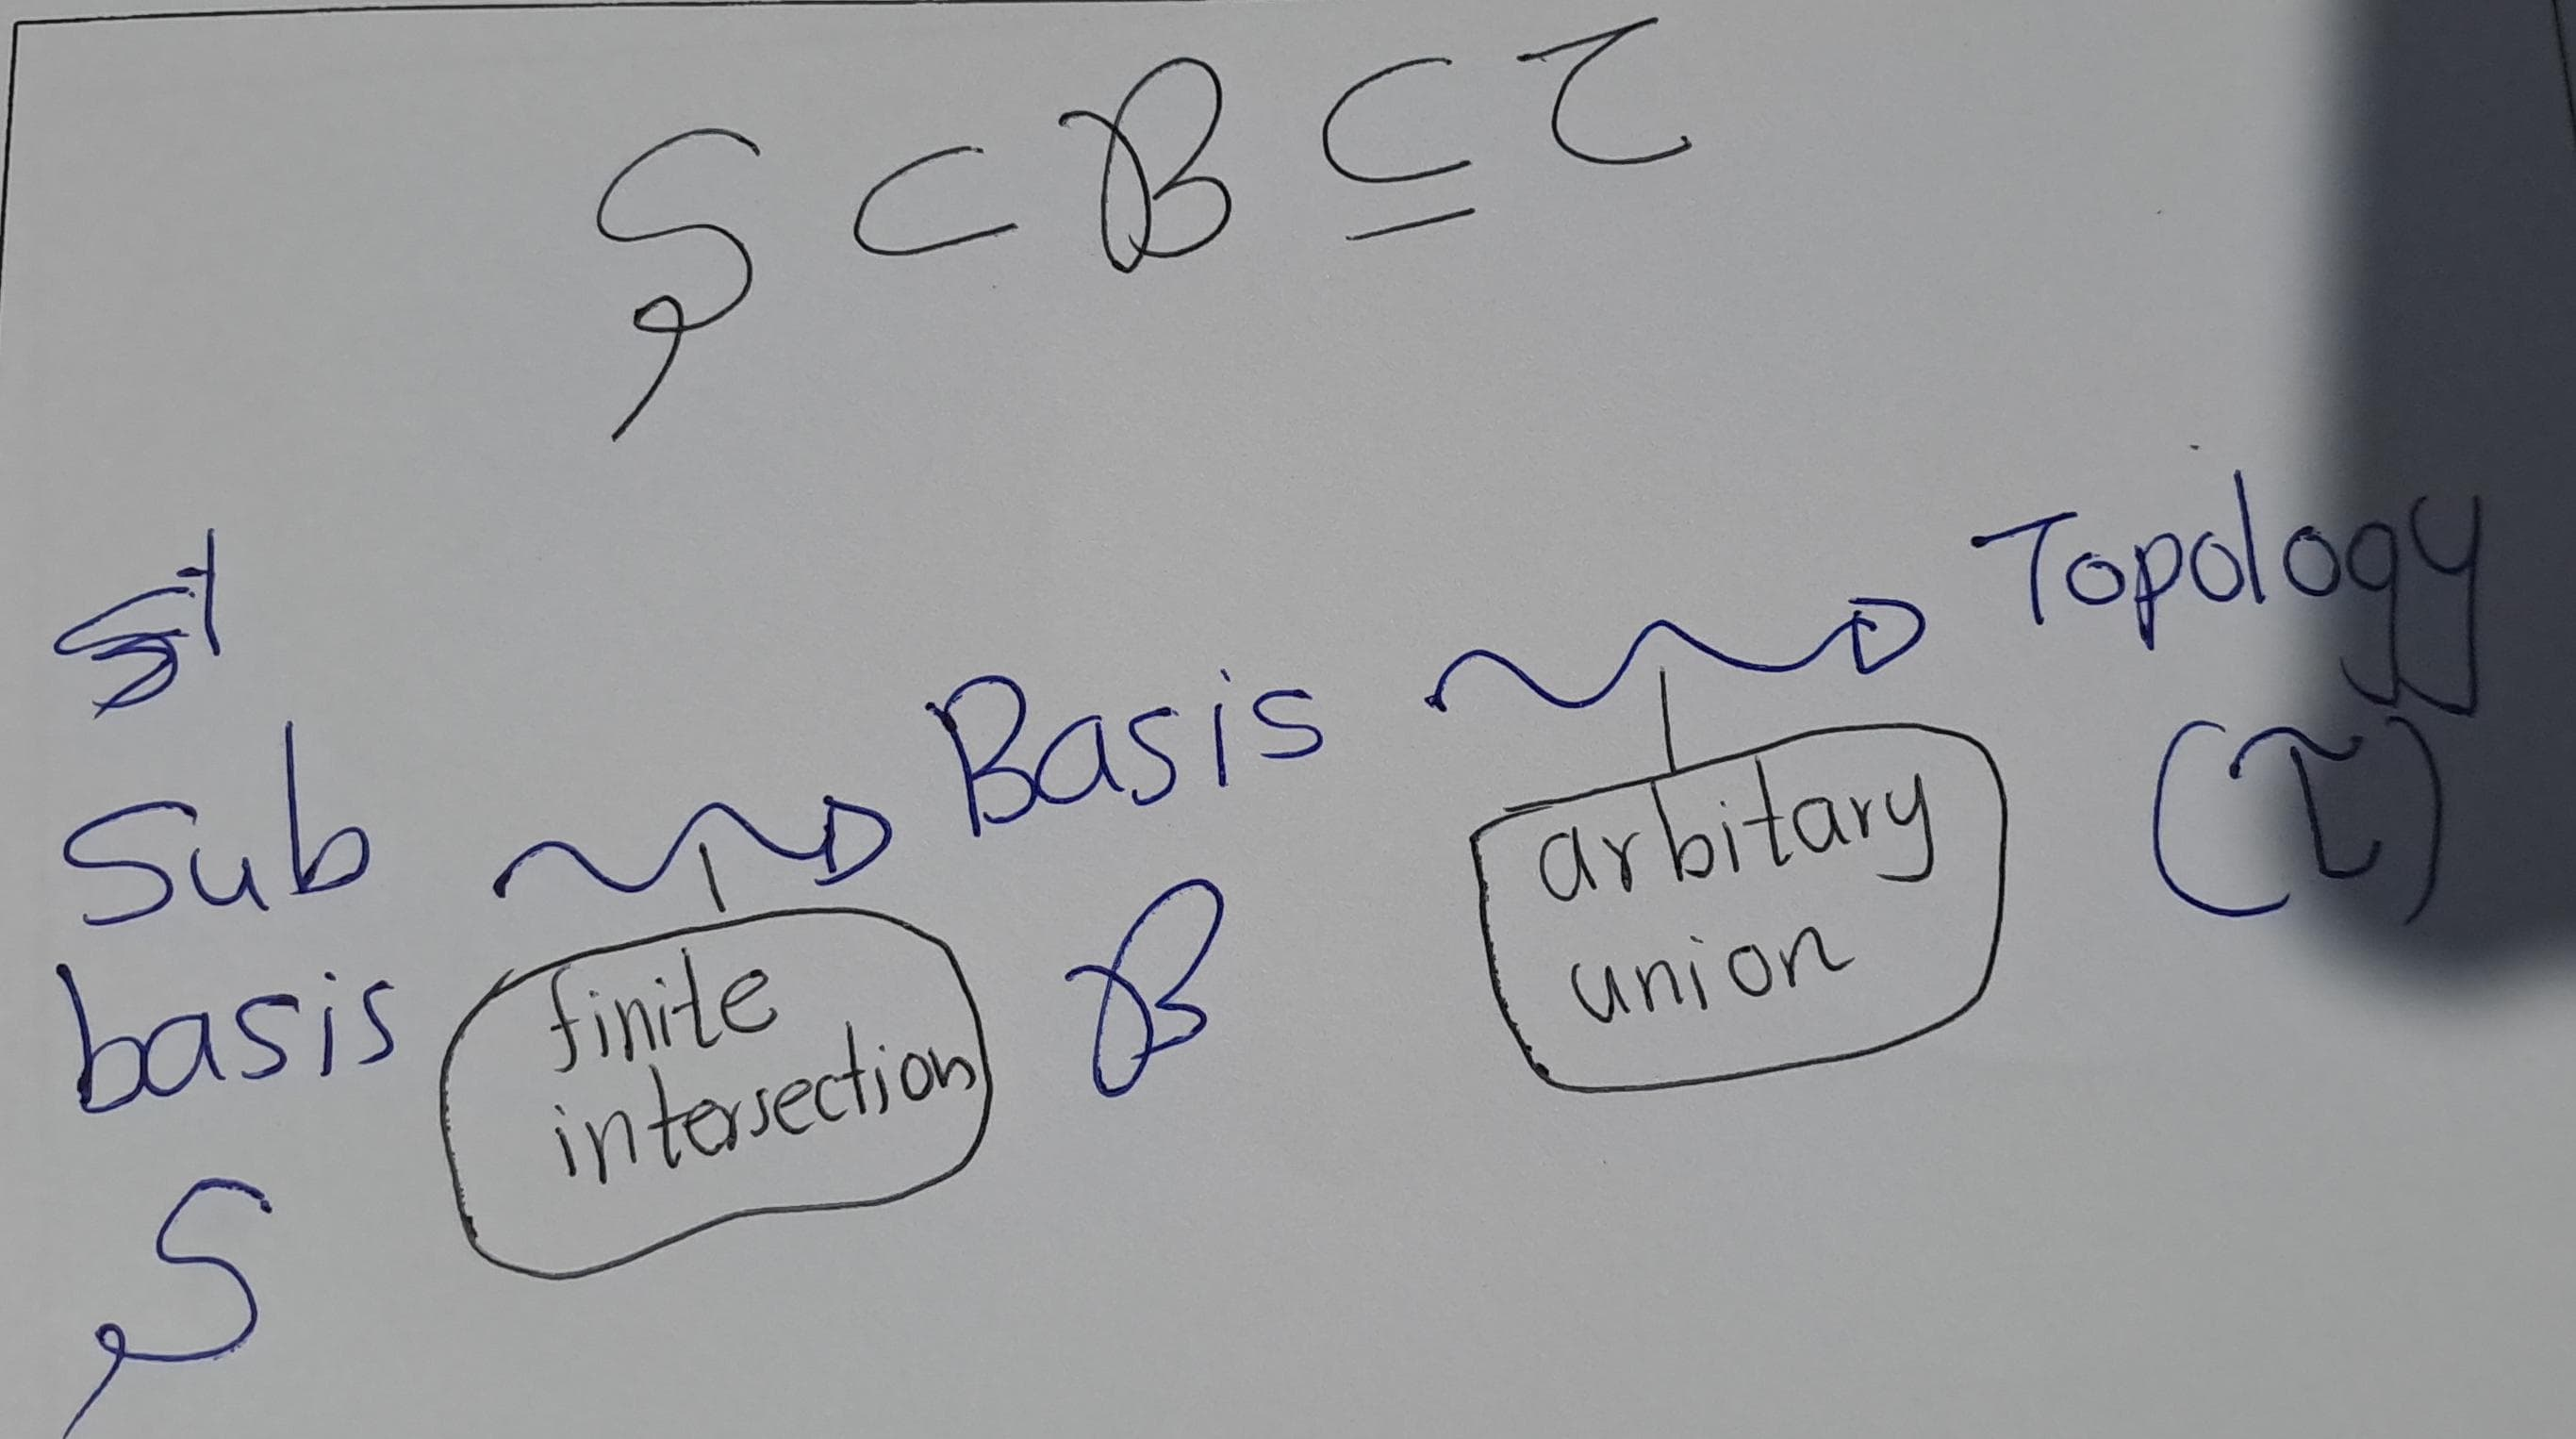
\includegraphics{figures/figure 06.jpg}
\caption{\label{fig:64}\(~\)}
\end{figure}

\begin{definition}
\protect\hypertarget{def:unnamed-chunk-19}{}\label{def:unnamed-chunk-19}The topology generated by the subbasis \(\mathcal{S}\) is defined to be the collection \(\mathcal{T}\) of all unions of finite intersections of elements of \(\mathcal{S}\).
\end{definition}

\hypertarget{order-topology}{%
\section{Order Topology}\label{order-topology}}

\begin{definition}[Linear Order/ Complete Order]
\protect\hypertarget{def:unnamed-chunk-20}{}\label{def:unnamed-chunk-20}

Consider order relation ``\(<\)''.

\begin{enumerate}
\def\labelenumi{\arabic{enumi}.}
\tightlist
\item
  If \(x \neq y\), then either \(x < y\) or \(y < x\).
\item
  If \(x < y\), then \(x\neq y\).
\item
  If \(x < y\) and \(y < z\), then \(x < z\).
\end{enumerate}

\end{definition}

\begin{example}
\protect\hypertarget{exm:unnamed-chunk-21}{}\label{exm:unnamed-chunk-21}\(\mathbb{R}\) is ordered set with less than relation.
\end{example}

First, let's see intervals in an Ordered Set.

Suppose that \(X\) is a set having a simple order relation \(<\). Given elements \(a\) and \(b\) of \(X\) such that \(a < b\), there are four subsets of \(X\) that are called the intervals determined by \(a\) and \(b\). They are the following :

\begin{itemize}
\tightlist
\item
  \((a, b) = \{x\in X | a < x < b\}\) (Type: open interval in \(X\)),
\item
  \((a, b] = \{x\in X | a < x ≤ b\}\)(Type: half-open interval in \(X\)),
\item
  \([a, b) = \{x\in X | a ≤ x < b\}\)(Type: half-open interval in \(X\)),
\item
  \([a, b] = \{x\in X | a ≤ x ≤ b\}\) (Type: closed interval in \(X\)),
\end{itemize}

The notation used here is familiar to you already in the case where \(X\) is the real line,but these are intervals in an arbitrary ordered set.

The use of the term ``open'' in this connection suggests that open intervals in \(X\) should turn out to be open sets when we put a topology on \(X\). And so they will.

\begin{definition}
\protect\hypertarget{def:unnamed-chunk-22}{}\label{def:unnamed-chunk-22}Let \(X\) be a set with a simple order relation; assume \(X\) has more than one element. Let \(\mathcal{B}\) be the collection of all sets of the following types:

\begin{enumerate}
\def\labelenumi{\arabic{enumi}.}
\tightlist
\item
  All open intervals \((a, b)\) in \(X\).
\item
  All intervals of the form \([a_0, b)\), where \(a_0\) is the smallest element (if any) of \(X\).
\item
  All intervals of the form \((a, b_0]\), where \(b_0\) is the largest element (if any) of \(X\).
\end{enumerate}

i.e.:
\[\begin{aligned}
\mathcal{B}:=&\{(a,b):a<b, a,b\in X\}\\
& \bigcup \{[a,b:a<b, a_0,b\in X \text{ and if $X$ has a smallest element and $a_0$ is the smallest element}\}\\
& \bigcup \{(a,b]:a<b, a,b_0\in X \text{ and if $X$ has a largest element and $b_0$ is the largest element}\}
\end{aligned}\]
The collection \(\mathcal{B}\) is a basis for a topology on \(X\), which is called the order topology.
\end{definition}

\textbf{Notation}: Denote an arbitrary element of \(\mathbb{R} \times \mathbb{R}\) by \(x \times y\), to avoid difficulty with notation.

\begin{definition}[Dictionary Oreder]
\protect\hypertarget{def:unnamed-chunk-23}{}\label{def:unnamed-chunk-23}Suppose that \(A\) and \(B\) are two sets with order relations \(<_{A}\) and \(<_{B}\) respectively. Define an order relation \(<\) on \(A \times B\) by defining \(a_{1} \times b_{1} < a_{2} \times b_{2}\) if \(a_{1} <_{A} a_{2}\), or if \(a_{1} = a_{2}\) and \(b_{1} <_{B} b_{2}\). It is called the dictionary order relation on \(A \times B\).
\end{definition}

\begin{example}
\protect\hypertarget{exm:unnamed-chunk-24}{}\label{exm:unnamed-chunk-24}Consider the set \(\mathbb{R} \times \mathbb{R}\) in the dictionary order. The set \(\mathbb{R} \times \mathbb{R}\) has neither a largest nor a smallest element, so the order topology on \(\mathbb{R} \times \mathbb{R}\) has as basis the collection of all open intervals of the form \((a \times b, c \times d)\) for \(a < c\), and for \(a = c\) and \(b < d\).

These two types of intervals are indicated in Figure 14.1. The sub collection consisting of only intervals of the second type is also a basis for the order topology on \(\mathbb{R} \times \mathbb{R}\), as you can check.
\end{example}

\begin{figure}
\centering
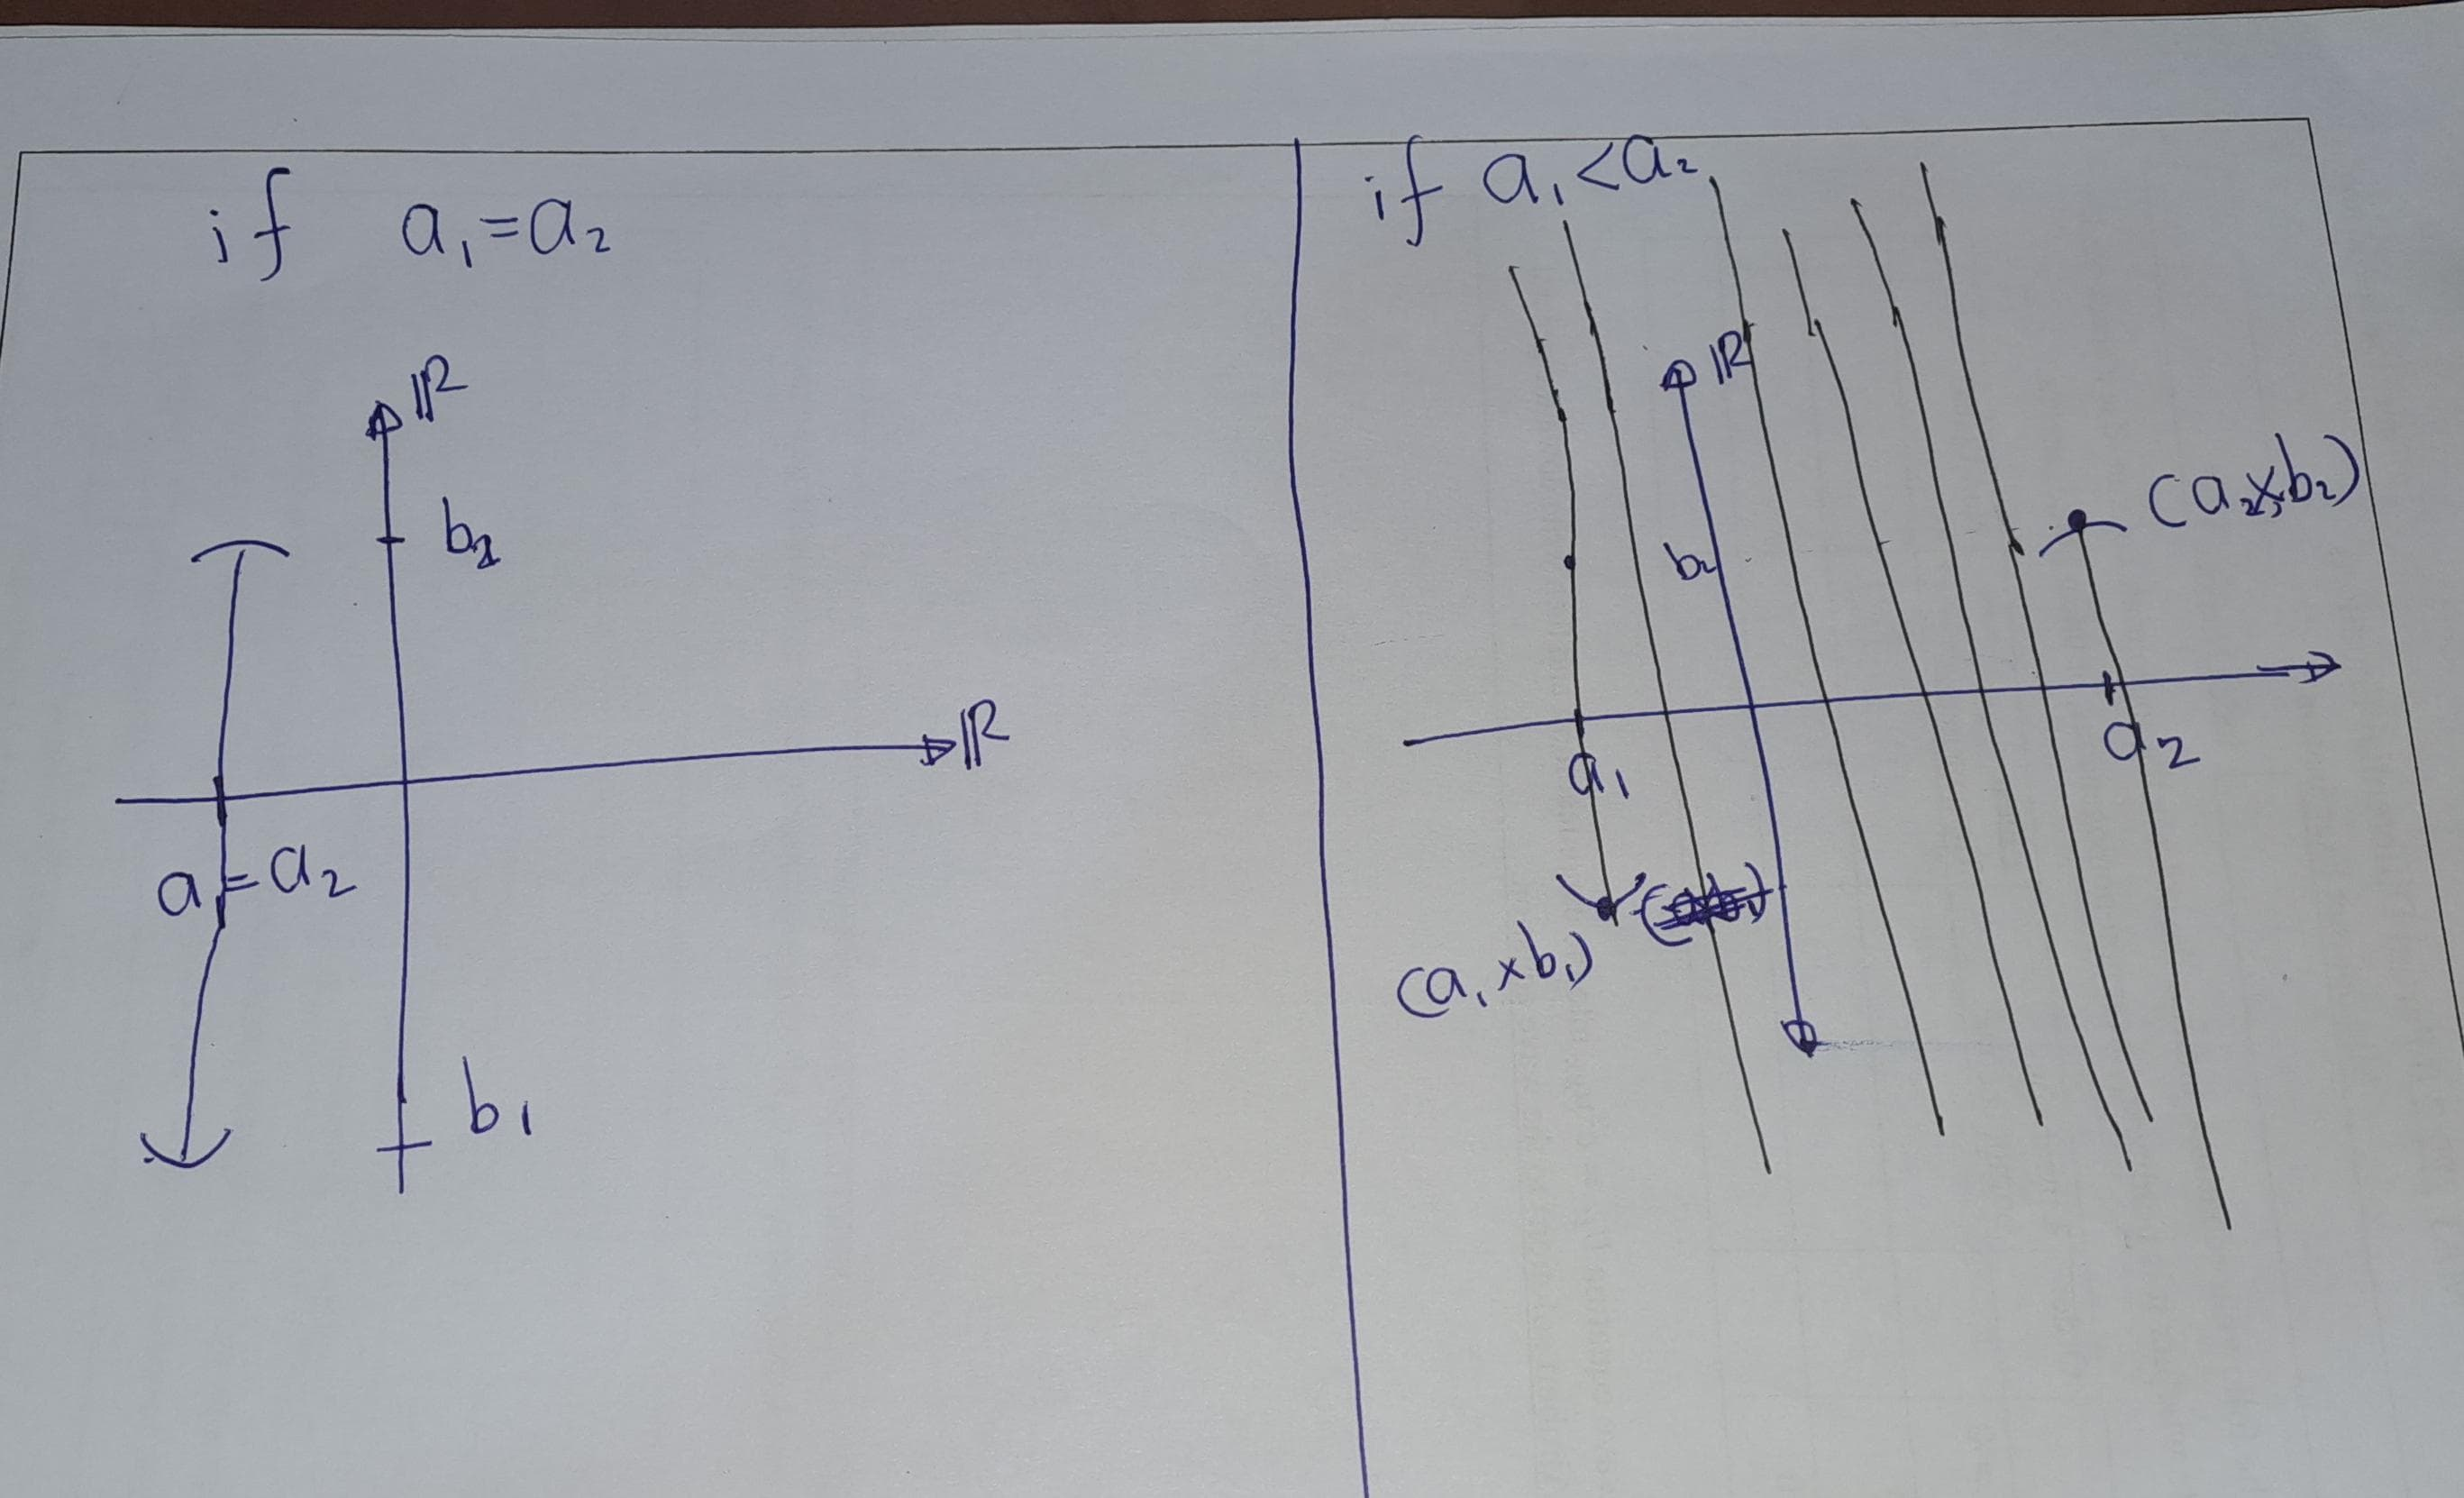
\includegraphics{figures/figure 07.jpg}
\caption{\label{fig:fi7}\(~\)}
\end{figure}

\begin{example}
\protect\hypertarget{exm:unnamed-chunk-25}{}\label{exm:unnamed-chunk-25}The standard topology,lower limit topology and upper limit topology on \(\mathbb{R}\).

\[\mathcal{B}:=\{(x,y):x<y, x,y\in \mathbb{R}\}\]
\(\mathcal{B}\) is a basis which generates the standard topology.
\[\mathcal{B}^\prime:=\{[x,y):x<y, x,y\in \mathbb{R}\}\]
\(\mathcal{B}^\prime\) is a basis which generates the lower limit topology on \(\mathbb{R}\).
\[\mathcal{B}^{\prime \prime}:=\{(x,y]:x<y, x,y\in \mathbb{R}\}\]
\(\mathcal{B}^{\prime \prime}\) is a basis which generates the upper limit topology on \(\mathbb{R}\).
\end{example}

\begin{lemma}
\protect\hypertarget{lem:unnamed-chunk-26}{}\label{lem:unnamed-chunk-26}The lower limit topology on \(\mathbb{R}\) is strictly finer than standard topology on \(\mathbb{R}\).
\end{lemma}

\begin{proof}
Let \((a,b)\in \mathbb{R}\). We are going to use Lemma \ref{lem:finerLemma}. Let \((a,b)\) be a element from basis of standard topology. Let \(x\in (a,b)\). Then \(a<x<b\). Then observe that \(x\in [x,b)\subset (a,b)\). Note that \([x,b)\) is element of basis of lower limit topology. Thus, by lemma \ref{lem:finerLemma} the lower limit topology on \(\mathbb{R}\) is finer than standard topology on \(\mathbb{R}\). Now we have to prove that \textbf{strictly property}.

Now let \([c,d)\) is element of basis of lower limit topology on \(\mathbb{R}\). Now observe that there is no open interval that containing \(c\) and contained in \([c,d)\). By lemma \ref{lem:finerLemma}, the lower limit topology on \(\mathbb{R}\) is strictly finer than standard topology on \(\mathbb{R}\).
\end{proof}

Note that basis element in lower limit topology is \textbf{not} open in the standard topology. But other way around is very true. As an example, \[(1,2)=\bigcup_{n\in \mathbb{N}}[1+\frac{1}{n},2).\] Clearly left hand side is open in lower limit topology by T2.

\begin{corollary}
\protect\hypertarget{cor:unnamed-chunk-28}{}\label{cor:unnamed-chunk-28}The lower limit topology on \(\mathbb{R}\) is not comparable upper limit topology on \(\mathbb{R}\).
\end{corollary}

\begin{proof}
Exercise

Hint: (try to find counter example)
\end{proof}

\textbf{Notation}:

\begin{itemize}
\tightlist
\item
  \(\mathbb{R}_l:=\mathbb{R}\) with lower limit topology.
\item
  \(\mathbb{R}_u:=\mathbb{R}\) with upper limit topology.
\item
  \(\mathbb{R}:=\mathbb{R}\) with standard topology.
\end{itemize}

\begin{example}
\protect\hypertarget{exm:unnamed-chunk-30}{}\label{exm:unnamed-chunk-30}The positive integers \(\mathbb{Z}^+:=\{1,2,3,...\}\) form an ordered set with a smallest element. The order topology on \(\mathbb{Z}^+\) is the discrete topology, for every one-point set is open: If \(n > 1\), then the one-point set \(\{n\} = (n - 1, n + 1)\) is a basis element; and if \(n = 1\), the one-point set \(\{1\}=[1, 2)\) is a basis element.
\end{example}

\begin{figure}
\centering
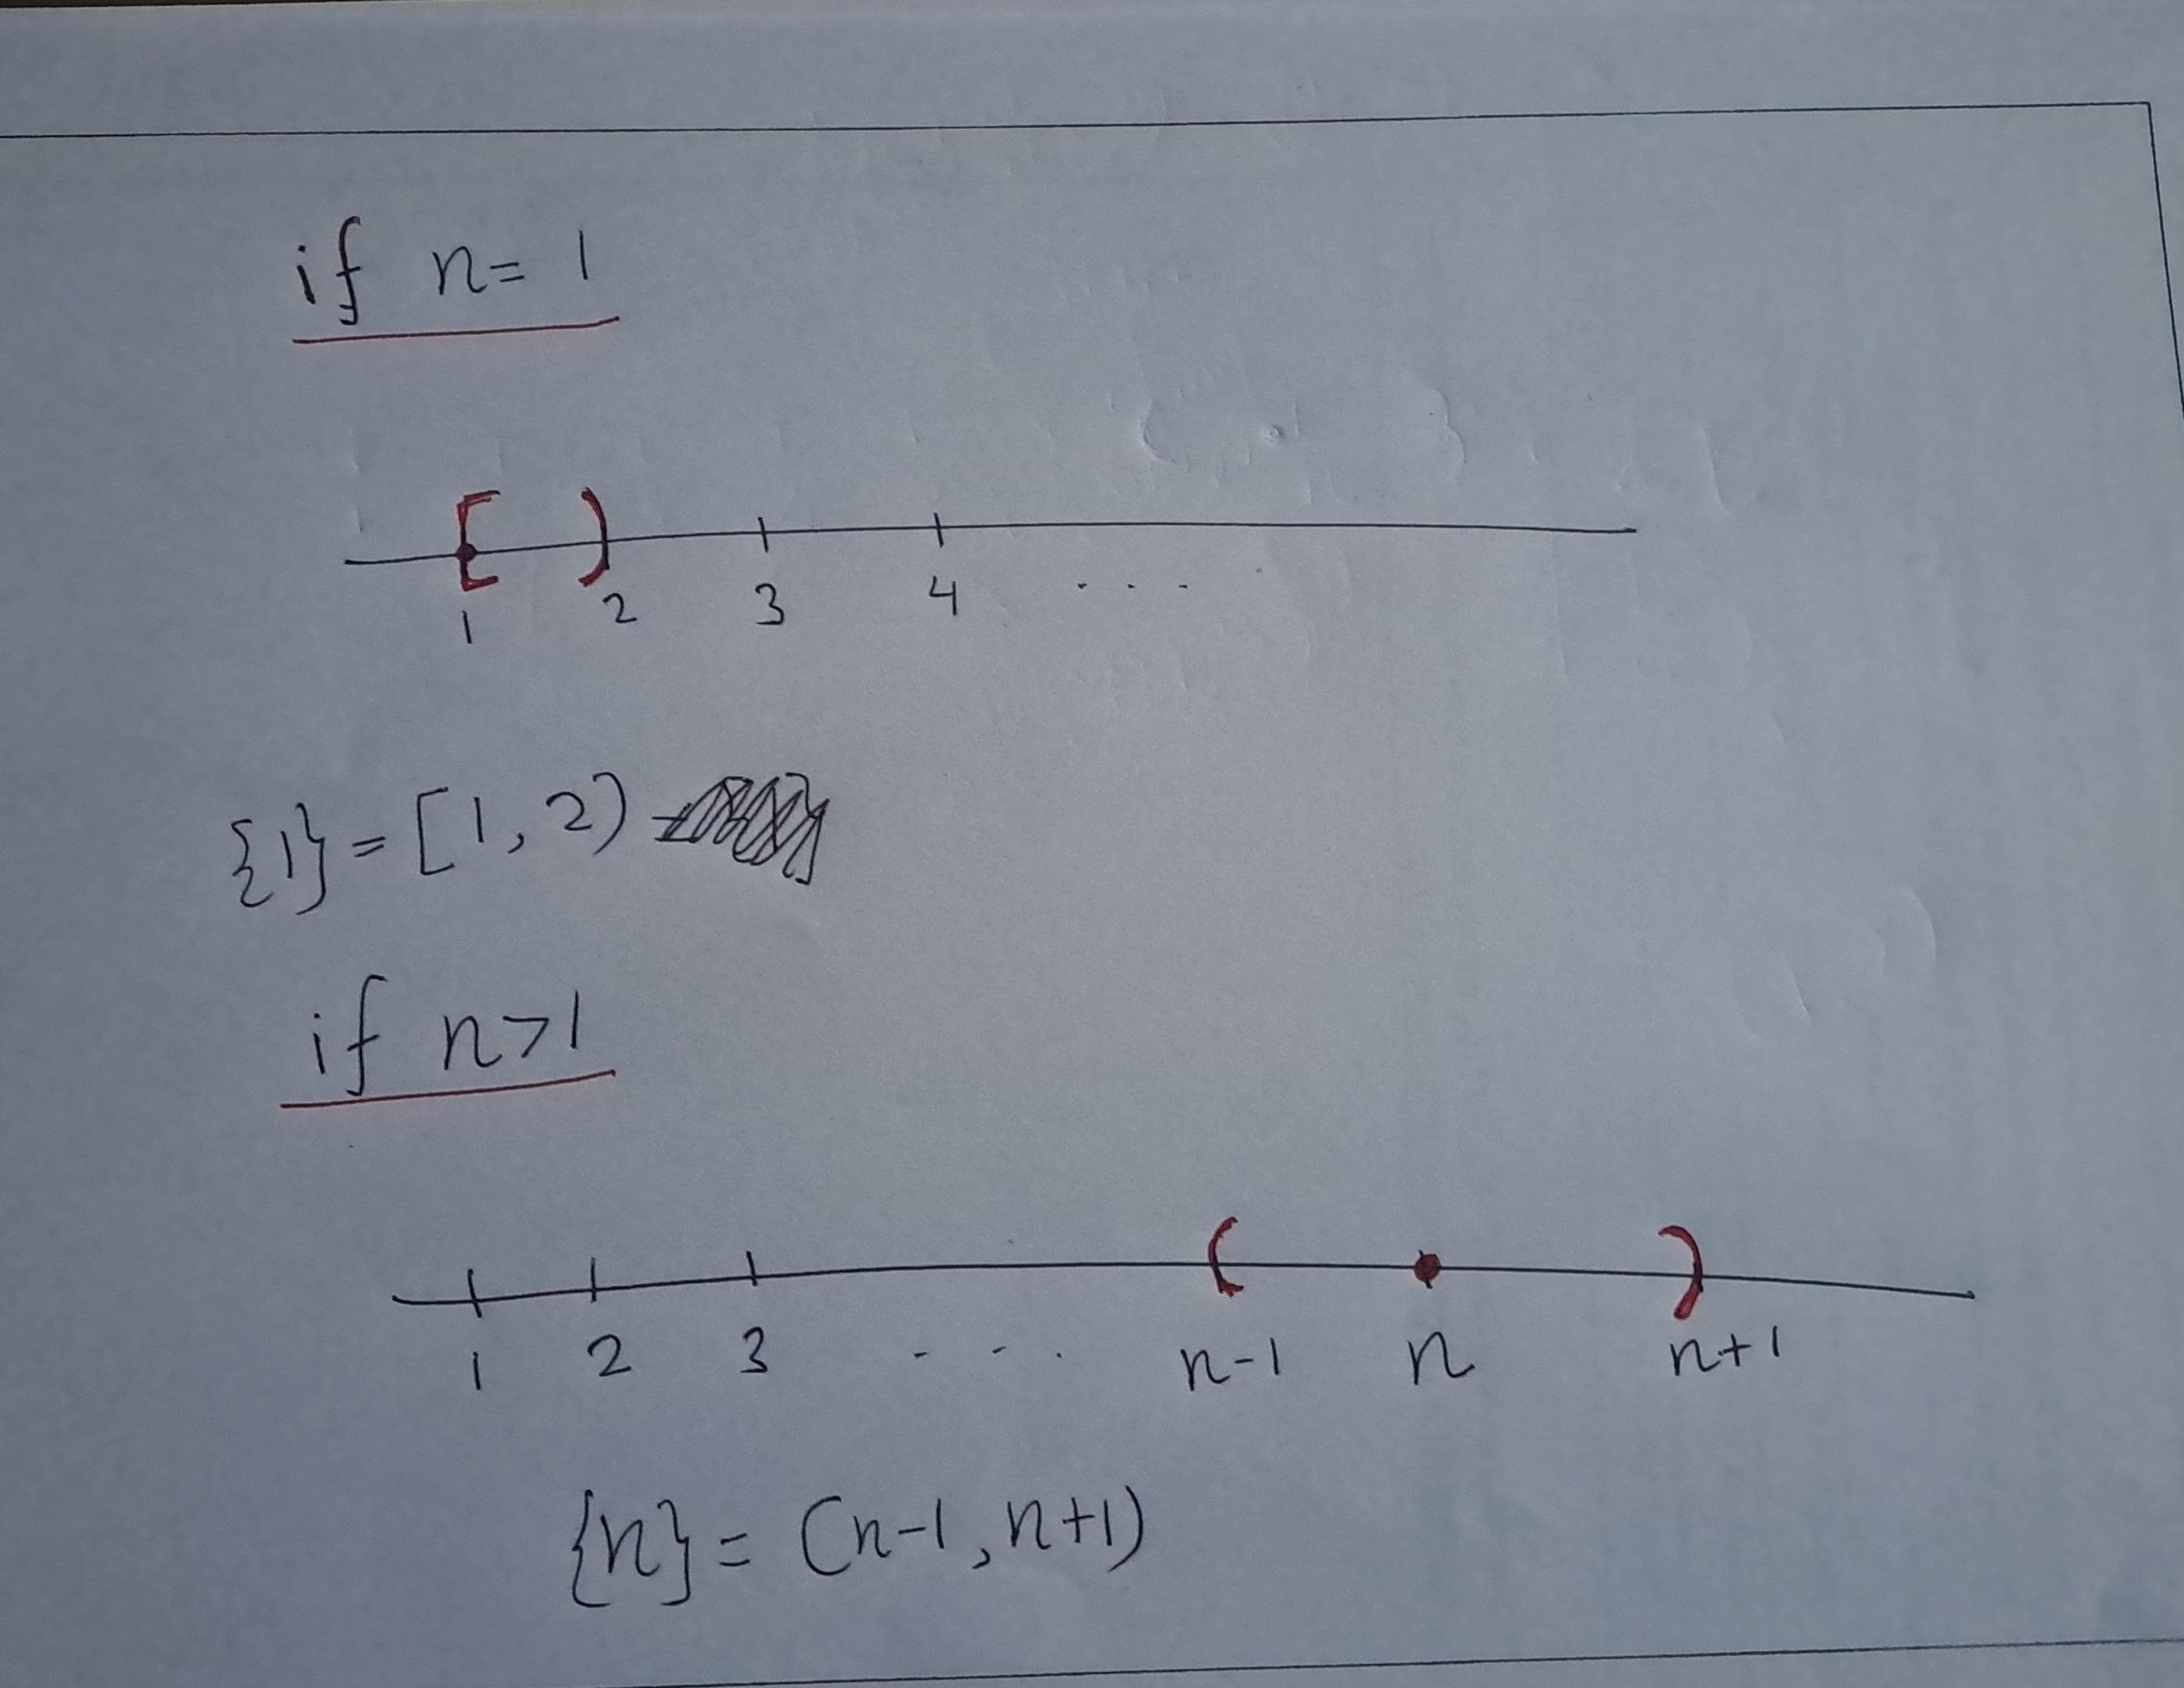
\includegraphics{figures/figure 08.jpg}
\caption{\label{fig:fig8}\(~\)}
\end{figure}

\begin{example}
\protect\hypertarget{exm:unnamed-chunk-31}{}\label{exm:unnamed-chunk-31}The set \(X = \{1, 2\} \times \mathbb{Z}^+\) in the dictionary order is another example of an ordered set with a smallest element. Denoting \(1 \times n\) by \(a_n\) and \(2 \times n\) by \(b_n\), we can represent \(X\) by
\[a_1, a_2,..., b_1, b_2,....\]

i.e.:\[X=\{1\times 1,1 \times 2, 1 \times 3, ..., 2\times 1, 2 \times 2, ....\}\]
Here \(a_1=1\times 1\) is the smallest element in \(X\).

The order topology on \(X\) is \textbf{not} the discrete topology. Most one-point sets are open, but there is an exception-the one-point set \(\{b_1\}={2\times 1}\). Any open set containing \(b_1\) must contain a basis element about \(b_1\) (G1 condition), and any basis element containing \(b_1\) contains points of the \(a_i\) sequence.
As an example, \(b_1=2\times 1\in (1\times 7,2\times 8)\). Then the sequence \(a_8,a_9,a_{10},....=1\times 8,1\times 9, 1\times 10,...\) contained in \((a_7,b_8)=(1\times 7,2\times 8)\). So, we cannot find an open interval in \(X\) that contains \(b_1\) and is contained in \(\{b_1\}\).
\end{example}

\begin{example}
\protect\hypertarget{exm:unnamed-chunk-32}{}\label{exm:unnamed-chunk-32}\[\mathcal{B}^{\prime\prime\prime}:=\{[x,y]:x\leq y, x,y\in \mathbb{R}\}\]
\(\mathcal{B}^{\prime\prime\prime}\) is a basis which generates the discrete topology on \(\mathbb{R}\). Because, \(\{a\}=[a,a]\).
\end{example}

\hypertarget{product-toplogy-on-x-times-y.}{%
\section{\texorpdfstring{Product Toplogy on \(X \times Y\).}{Product Toplogy on X \textbackslash times Y.}}\label{product-toplogy-on-x-times-y.}}

The Cartesian product of two topological spaces has an induced topology called the product topology. There is also an induced basis for it. Here is the example to keep in mind:

\begin{example}
\protect\hypertarget{exm:egR2}{}\label{exm:egR2}Recall that the standard topology of \(\mathbb{R}^{2}\) is given by the basis

\[
\mathcal{B}:=\left\{(a, b) \times(c, d) \subset \mathbb{R}^{2} \mid a<b, c<d\right\}
\]
\end{example}

\begin{proof}
(Proof of \(\mathcal{B}\) is basis.)
- (B1) Let \((x,y)\in \mathbb{R}^2\). Then observe that \(x\in(x-1,x+1)\subseteq \mathbb{R}\), and \(y\in(y-1,y+1)\subseteq \mathbb{R}\). Thus
\[(x,y)\in (x-1,x+1)\times (y-1,y+1).\]

See figure \ref{fig:fig4}.
Therefore, this satisfied the B1 condition.

\begin{itemize}
\tightlist
\item
  Now suppose that \((x,y)\in (a_1,b_1)\times(c_1,d_1)\cap (a_2,b_2)\times(c_2,d_2)\)
  Now observe
  \((x,y)\in (a_1,b_1)\times(c_1,d_1)\implies x\in(a_1,b_1)\) and \(y\in(c_1,d_1)\)
\end{itemize}

and

\((x,y)\in (a_2,b_2)\times(c_2,d_2)\implies x\in(a_2,b_2)\) and \(y\in(c_2,d_2)\)
Let \(a=\max\{a_1,a_2\},b=\min\{b_1,b_2\}, c=\max\{c_1,c_2\}\) and \(d=\min\{d_1,d_2\}\). Then observe that
\[x\in (a,b)\quad \text{and} y\in (c,d)\].
Further, \[(x,y)\in (a,b)\times (c,d)\subseteq (a_2,b_2)\times(c_2,d_2)\implies x\in(a_2,b_2)\].
See figure \ref{fig:fig5}.
This satisfies B2 condition.
\end{proof}

\begin{figure}
\centering
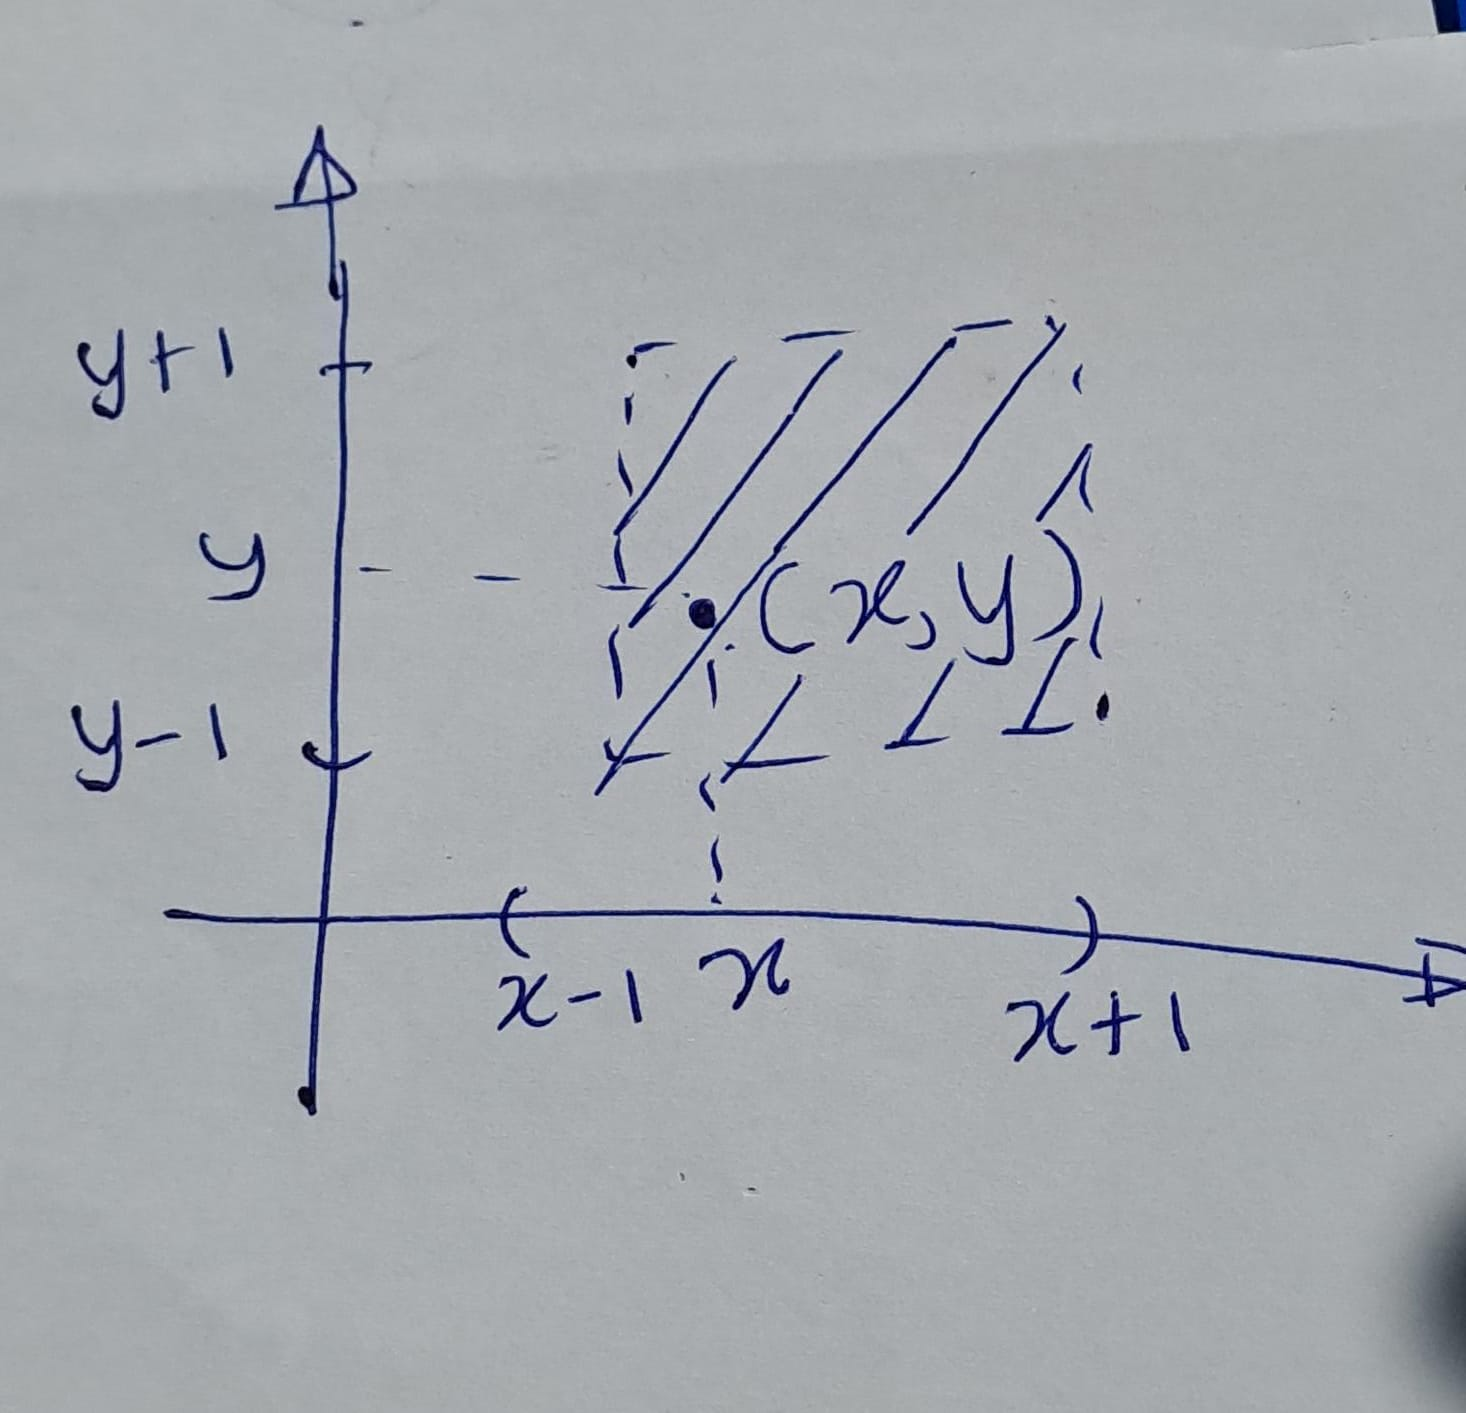
\includegraphics{figures/figure 04.jpg}
\caption{\label{fig:fig4}\(~\)}
\end{figure}

\begin{figure}
\centering
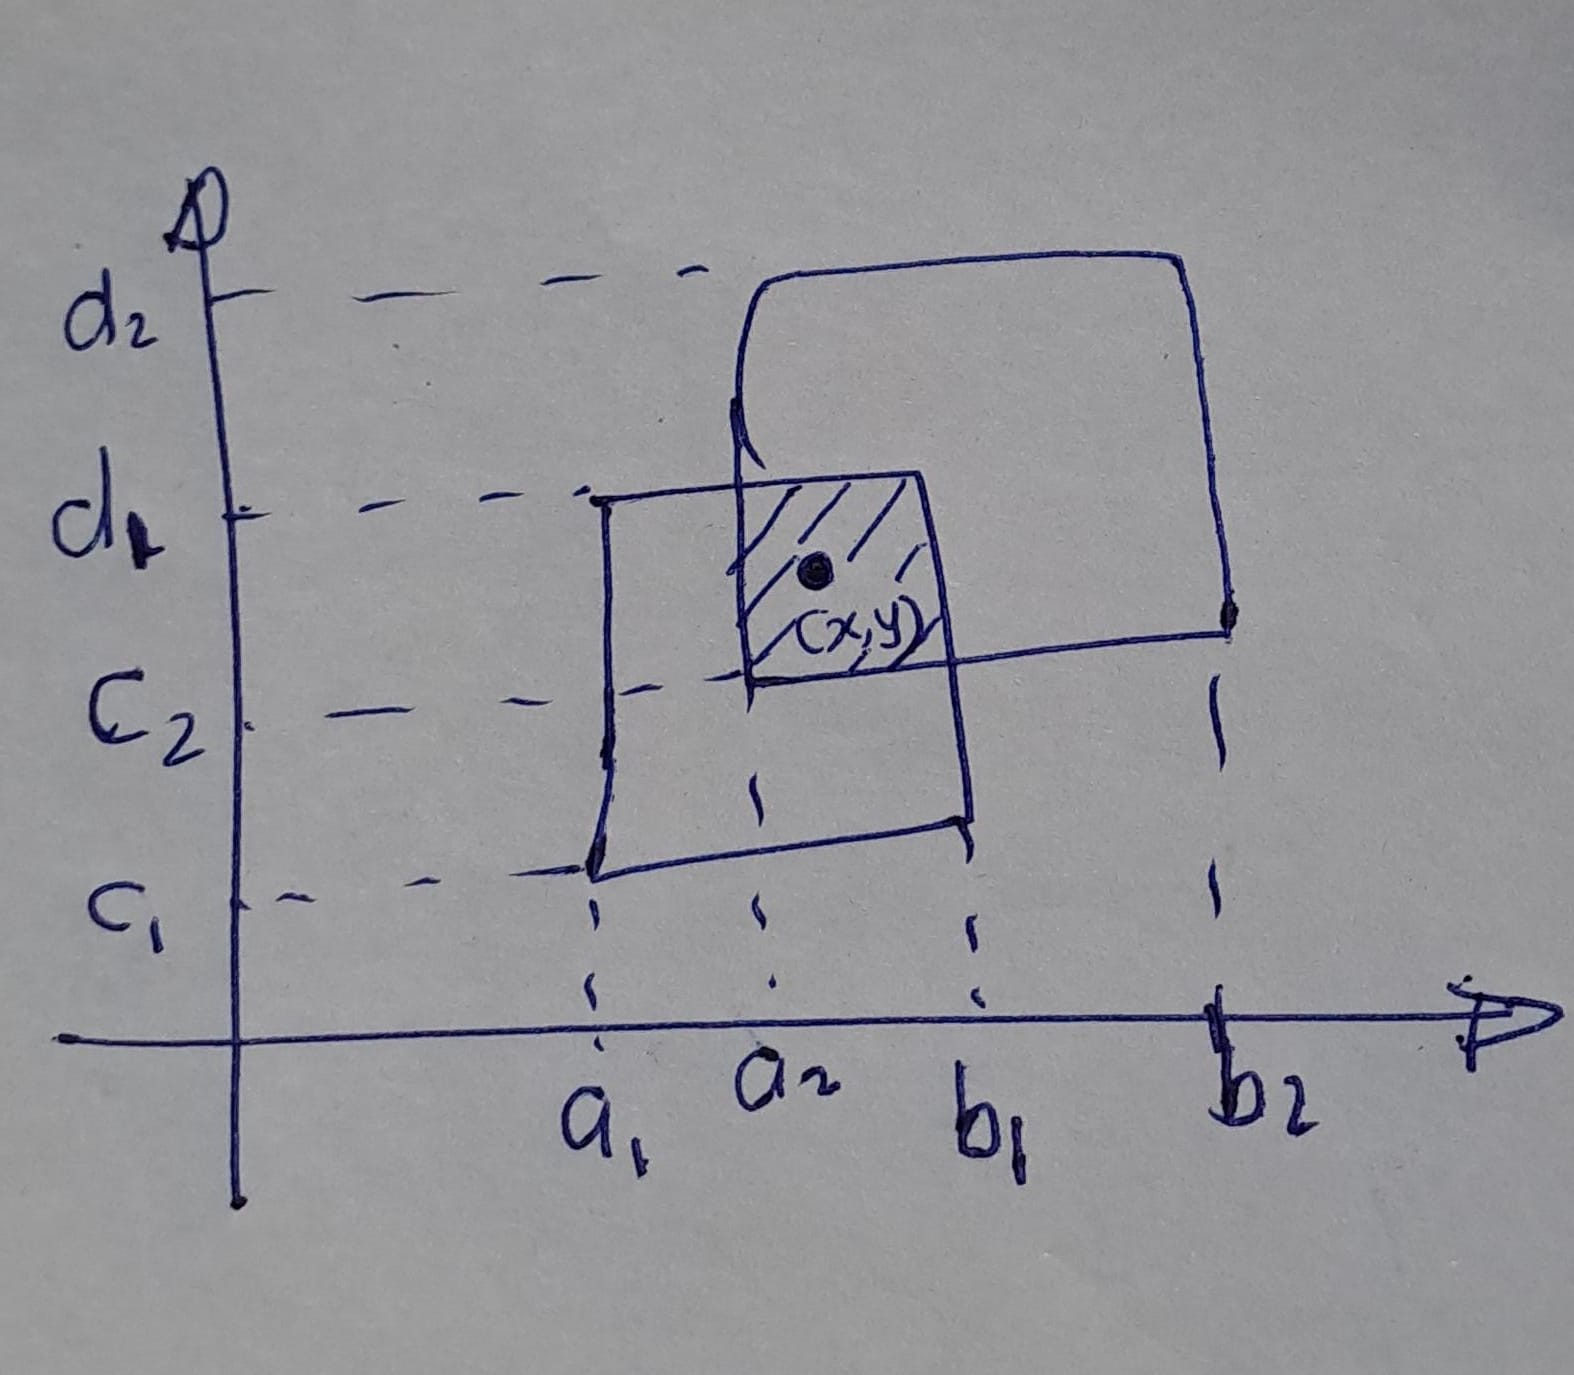
\includegraphics{figures/figure 05.jpg}
\caption{\label{fig:fig5}\(~\)}
\end{figure}

Let's go to a rigid definition.

\begin{definition}
\protect\hypertarget{def:unnamed-chunk-34}{}\label{def:unnamed-chunk-34}If \(\left(X, \mathcal{T}_{X}\right)\) and \(\left(Y, \mathcal{T}_{Y}\right)\) are topological spaces, then the collection \(\mathcal{B}\) of subsets of the form \(U \times V \subset X \times Y, U \in \mathcal{T}_{X}, V \in \mathcal{T}_{Y}\) forms a basis of a topology.

i.e.:
\[\mathcal{B}:=\{U \times V \subset X \times Y: U \in \mathcal{T}_{X}, V \in \mathcal{T}_{Y}\}\]
The topology generated by \(\mathcal{B}\) is called product topology on \(X \times Y\).
\end{definition}

\begin{proof}

(Proof of \(\mathcal{B}\) is basis)

\begin{itemize}
\item
  (B1) Let \((x, y) \in X \times Y\) be an arbitrary element. We need to find a subset in \(\mathcal{B}\) containing \((x, y)\), but since \(X \times Y \in \mathcal{B}\), it is obvious.
\item
  (B2) For any \(U_{1} \times V_{1}, U_{2} \times V_{2} \in \mathcal{B}\), the intersection is \(\left(U_{1} \times V_{1}\right) \cap\left(U_{2} \times V_{2}\right)=\left(U_{1} \cap U_{2}\right) \times\left(V_{1} \cap V_{2}\right) \in \mathcal{B}\). So it is obvious again.
\end{itemize}

\end{proof}

\begin{figure}
\centering
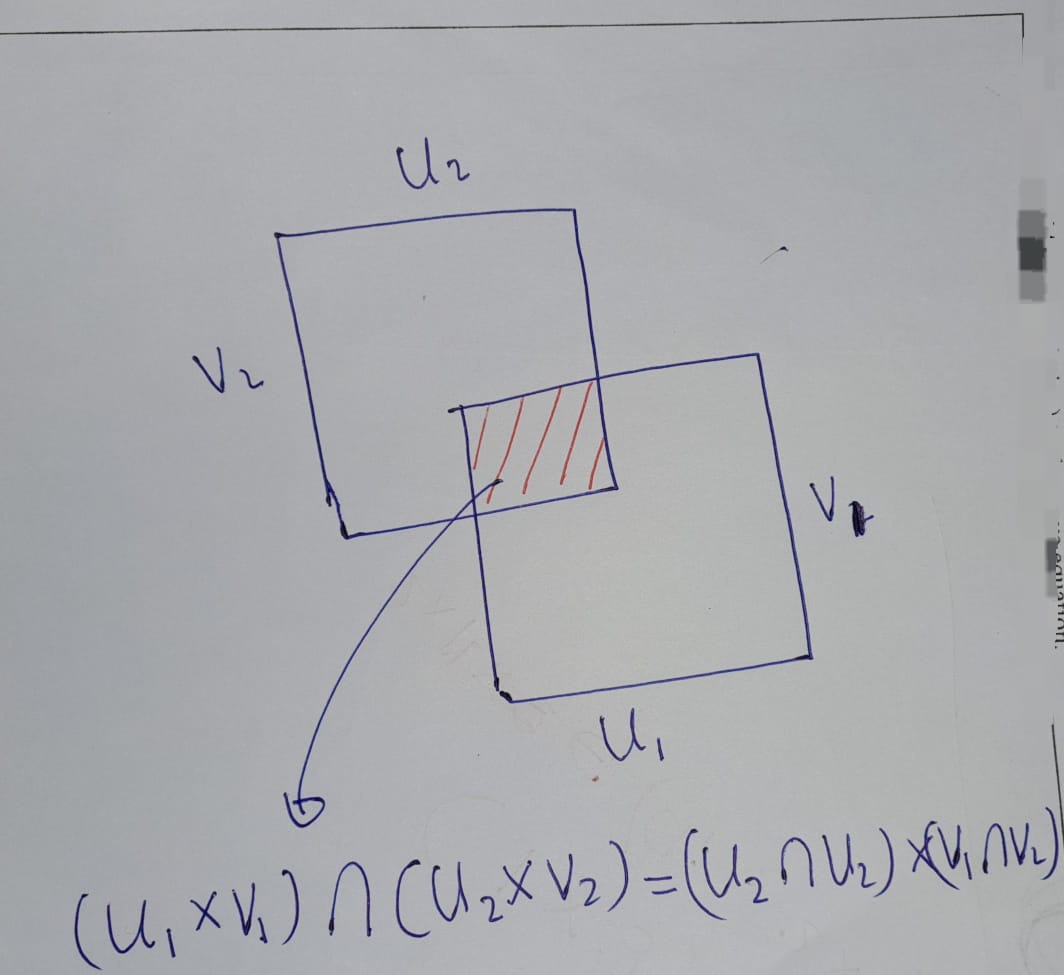
\includegraphics{figures/figure 09.jpg}
\caption{\label{fig:fig09}\(~\)}
\end{figure}

\begin{theorem}
\protect\hypertarget{thm:unnamed-chunk-36}{}\label{thm:unnamed-chunk-36}If \(\mathcal{B}_X\) is a basis of \((X, \mathcal{T}_X)\) and \(\mathcal{B}_Y\) is a basis of \((Y, \mathcal{T}_Y)\), then \(\mathcal{B}_X \times \mathcal{B}_Y\) is a basis of the product topology on \(X \times Y\).
\end{theorem}

\begin{proof}
To check \(\mathcal{B}_{X \times Y}\), let's use lemma \ref{lem:lemma110} which states that \(\mathcal{B}\) is a basis for \(\mathcal{T}\) iff for any \(U \in T\) and any \(x \in U\), there is \(B \in \mathcal{B}\) such that \(x \in B \subseteq U\).

Let \(W \in \mathcal{T}_{prod}\) and \((x, y) \in W\). By the definition of product topology, there are \(U \in \mathcal{T}_X\) and \(V \in \mathcal{T}_Y\) such that \((x,y) \in U \times V \subseteq W\). Since \(\mathcal{B}_X\) and \(\mathcal{B}_Y\) are bases, there are \(B \in \mathcal{B}_X\) and \(C \in \mathcal{B}_Y\) such that \(x \in B \subseteq U\) and \(y \in C \subseteq V\). Thus we found \(B \times C \in \mathcal{B}_{X \times Y}\) such that \((x,y) \in B \times C \subseteq W\).
\end{proof}

\begin{example}
\protect\hypertarget{exm:unnamed-chunk-38}{}\label{exm:unnamed-chunk-38}The standard topology on \(\mathbb{R}^2=\mathbb{R}\times\mathbb{R}\) is the product toplogy. (See example \ref{exm:egR2})

Obsereve that basis elements in product topology in \(\mathbb{R}^2\) are open recatngles (product of two open intervals.).
\end{example}

\begin{figure}
\centering
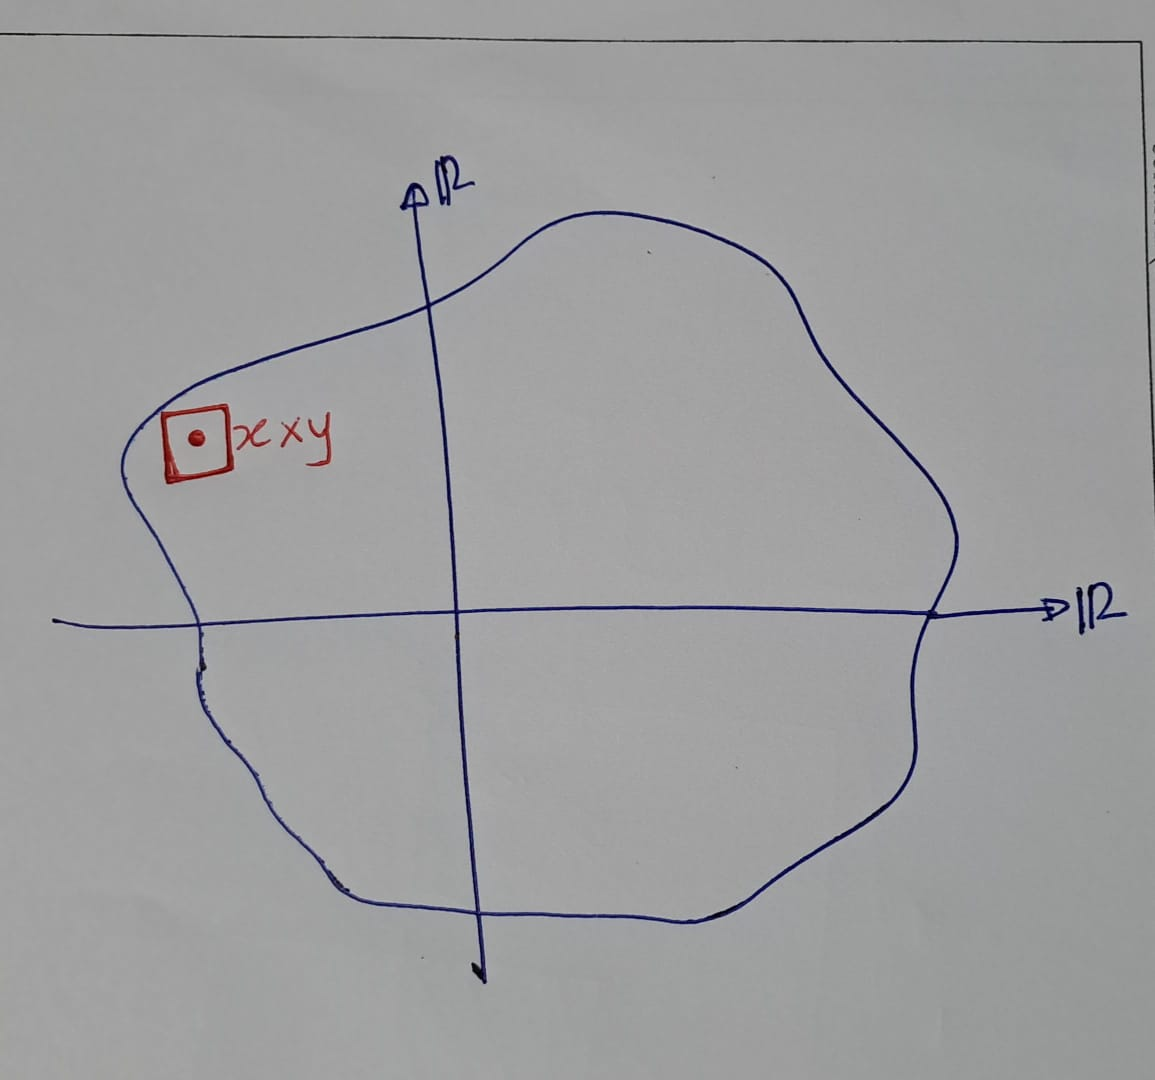
\includegraphics{figures/figure 10.jpg}
\caption{\label{fig:fig10}\(~\)}
\end{figure}

\begin{lemma}
\protect\hypertarget{lem:unnamed-chunk-39}{}\label{lem:unnamed-chunk-39}The dictionary topology \(\mathbb{R}^2\) is strictly finer than standard toplogy in \(\mathbb{R}^2\)
\end{lemma}

\begin{proof}
We are going to use \ref{lem:finerLemma}.
Let \((a,b)\times(c,d)\subset\mathbb{R}^2\) be a element of basis of standard toplogy on \(\mathbb{R}^2\), and let \(x\times y\in (a,b)\times (c,d)\). Now we need to find basis element of the dictionary order topology that contained in \((a,b)\times (c,d)\).
So,
\[x\times y \in (x\times c ,x\times d)\subset (a,b)\times(c,d).\]
Note that \((x\times c ,x\times d)\) is a basis element in the dictonary order topology. Now let's proove the stricly finer condition.

Let \((p\times q,p \times s)\) be basis element of order toplogy. Let \(p\times y \in (p\times q,p \times s)\). Now observe that there is no open rectangle that containing \(p\times y\) and contained in \((p\times q,p \times s)\). By lemma \ref{lem:finerLemma}, the order topology on \(\mathbb{R}^2\) is strictly finer than standard topology on \(\mathbb{R}^2\).
\end{proof}

\begin{figure}
\centering
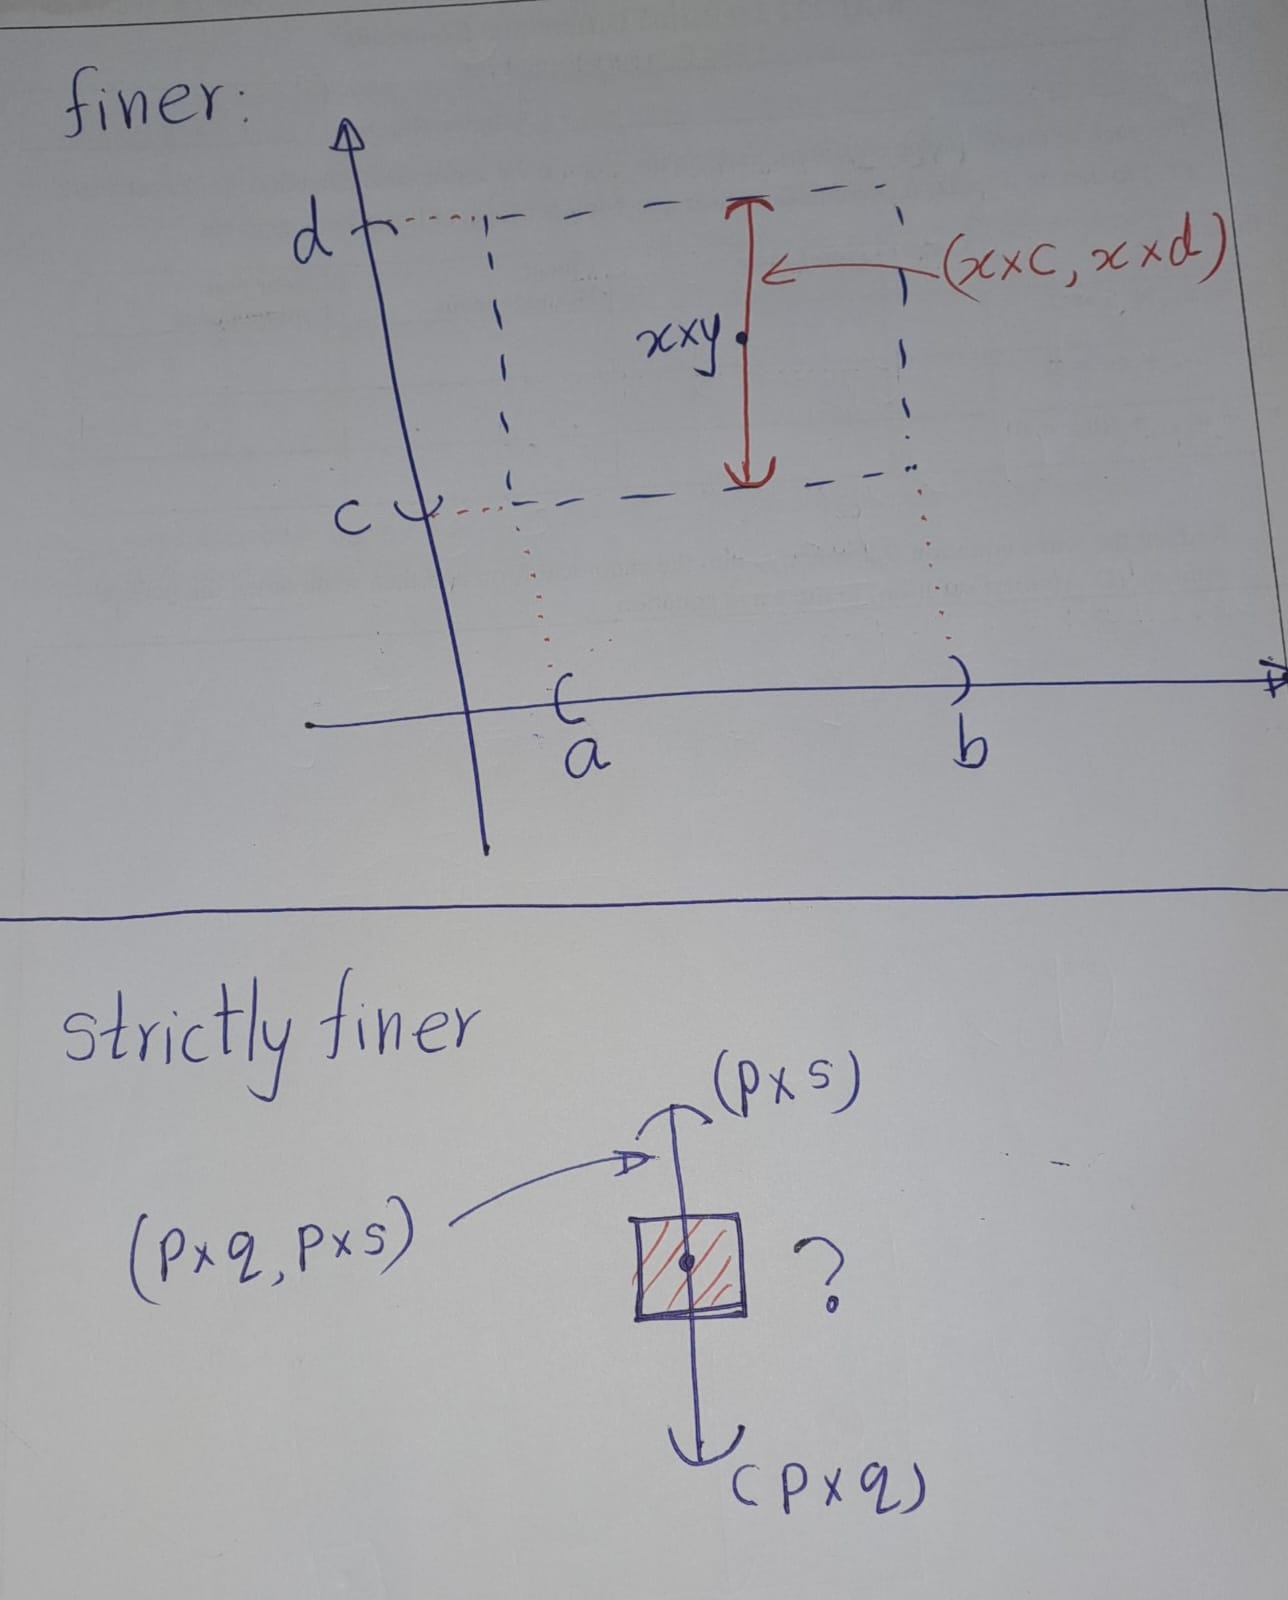
\includegraphics{figures/figure 11.jpg}
\caption{\label{fig:fig11}\(~\)}
\end{figure}

Now I am intersected in a problem. That is can we write dictionary order topology as \(\mathbb{R}^2\) as product topology. Actually we can, \[\mathbb{R}^2_{dictionary}:=\mathbb{R}_{discrete }\times \mathbb{R}_{standard}\]

\begin{proof}
Let \(\{a\} \times (c,d)\) be a basis element in product toplogy \(\mathbb{R}_d \times \mathbb{R}\). Let \(a\times x\in \{a\} \times (c,d)\) obsereve that
\[a\times x\in \{a\} \times (c,d) = (a\times c,a\times d)\]
and \((a\times c,a\times d)\) is basis element of order topology \(\mathbb{R}^2\). Thus by lemma \ref{lem:finerLemma}, order toplogy in \(\mathbb{R}^2\) is finer than the product toplogy \(\mathbb{R}_d \times \mathbb{R}\).

Now suppose that \((p\times q, r \times s)\) be a basis elemenet in order toplogy on \(\mathbb{R}^2\).

\begin{itemize}
\tightlist
\item
  If \(p<x\), define \(l=y−1\) and if \(p=x\) define \(l=r\). In either case we know that \((p\times q)<(x\times l)<(x\times y)\).
\item
  If \(x<r\) define \(t=y+1\) and if \(x=r\) define \(t=s\). In either case we know that \((x\times y)<(x\times t)<(q \times s)\).
\end{itemize}

See figure \ref{fig:fig12}
So \[(x,y) \in \{x\} \times (l,t) \subseteq (p \times q, r \times s).\]
Thus by lemma \ref{lem:finerLemma}, product toplogy \(\mathbb{R}_d \times \mathbb{R}\) is finer than order toplogy in \(\mathbb{R}^2\).

Therefore, \[\mathbb{R}^2_{dictionary}=\mathbb{R}_{discrete }\times \mathbb{R}_{standard}\]
\end{proof}

\begin{figure}
\centering
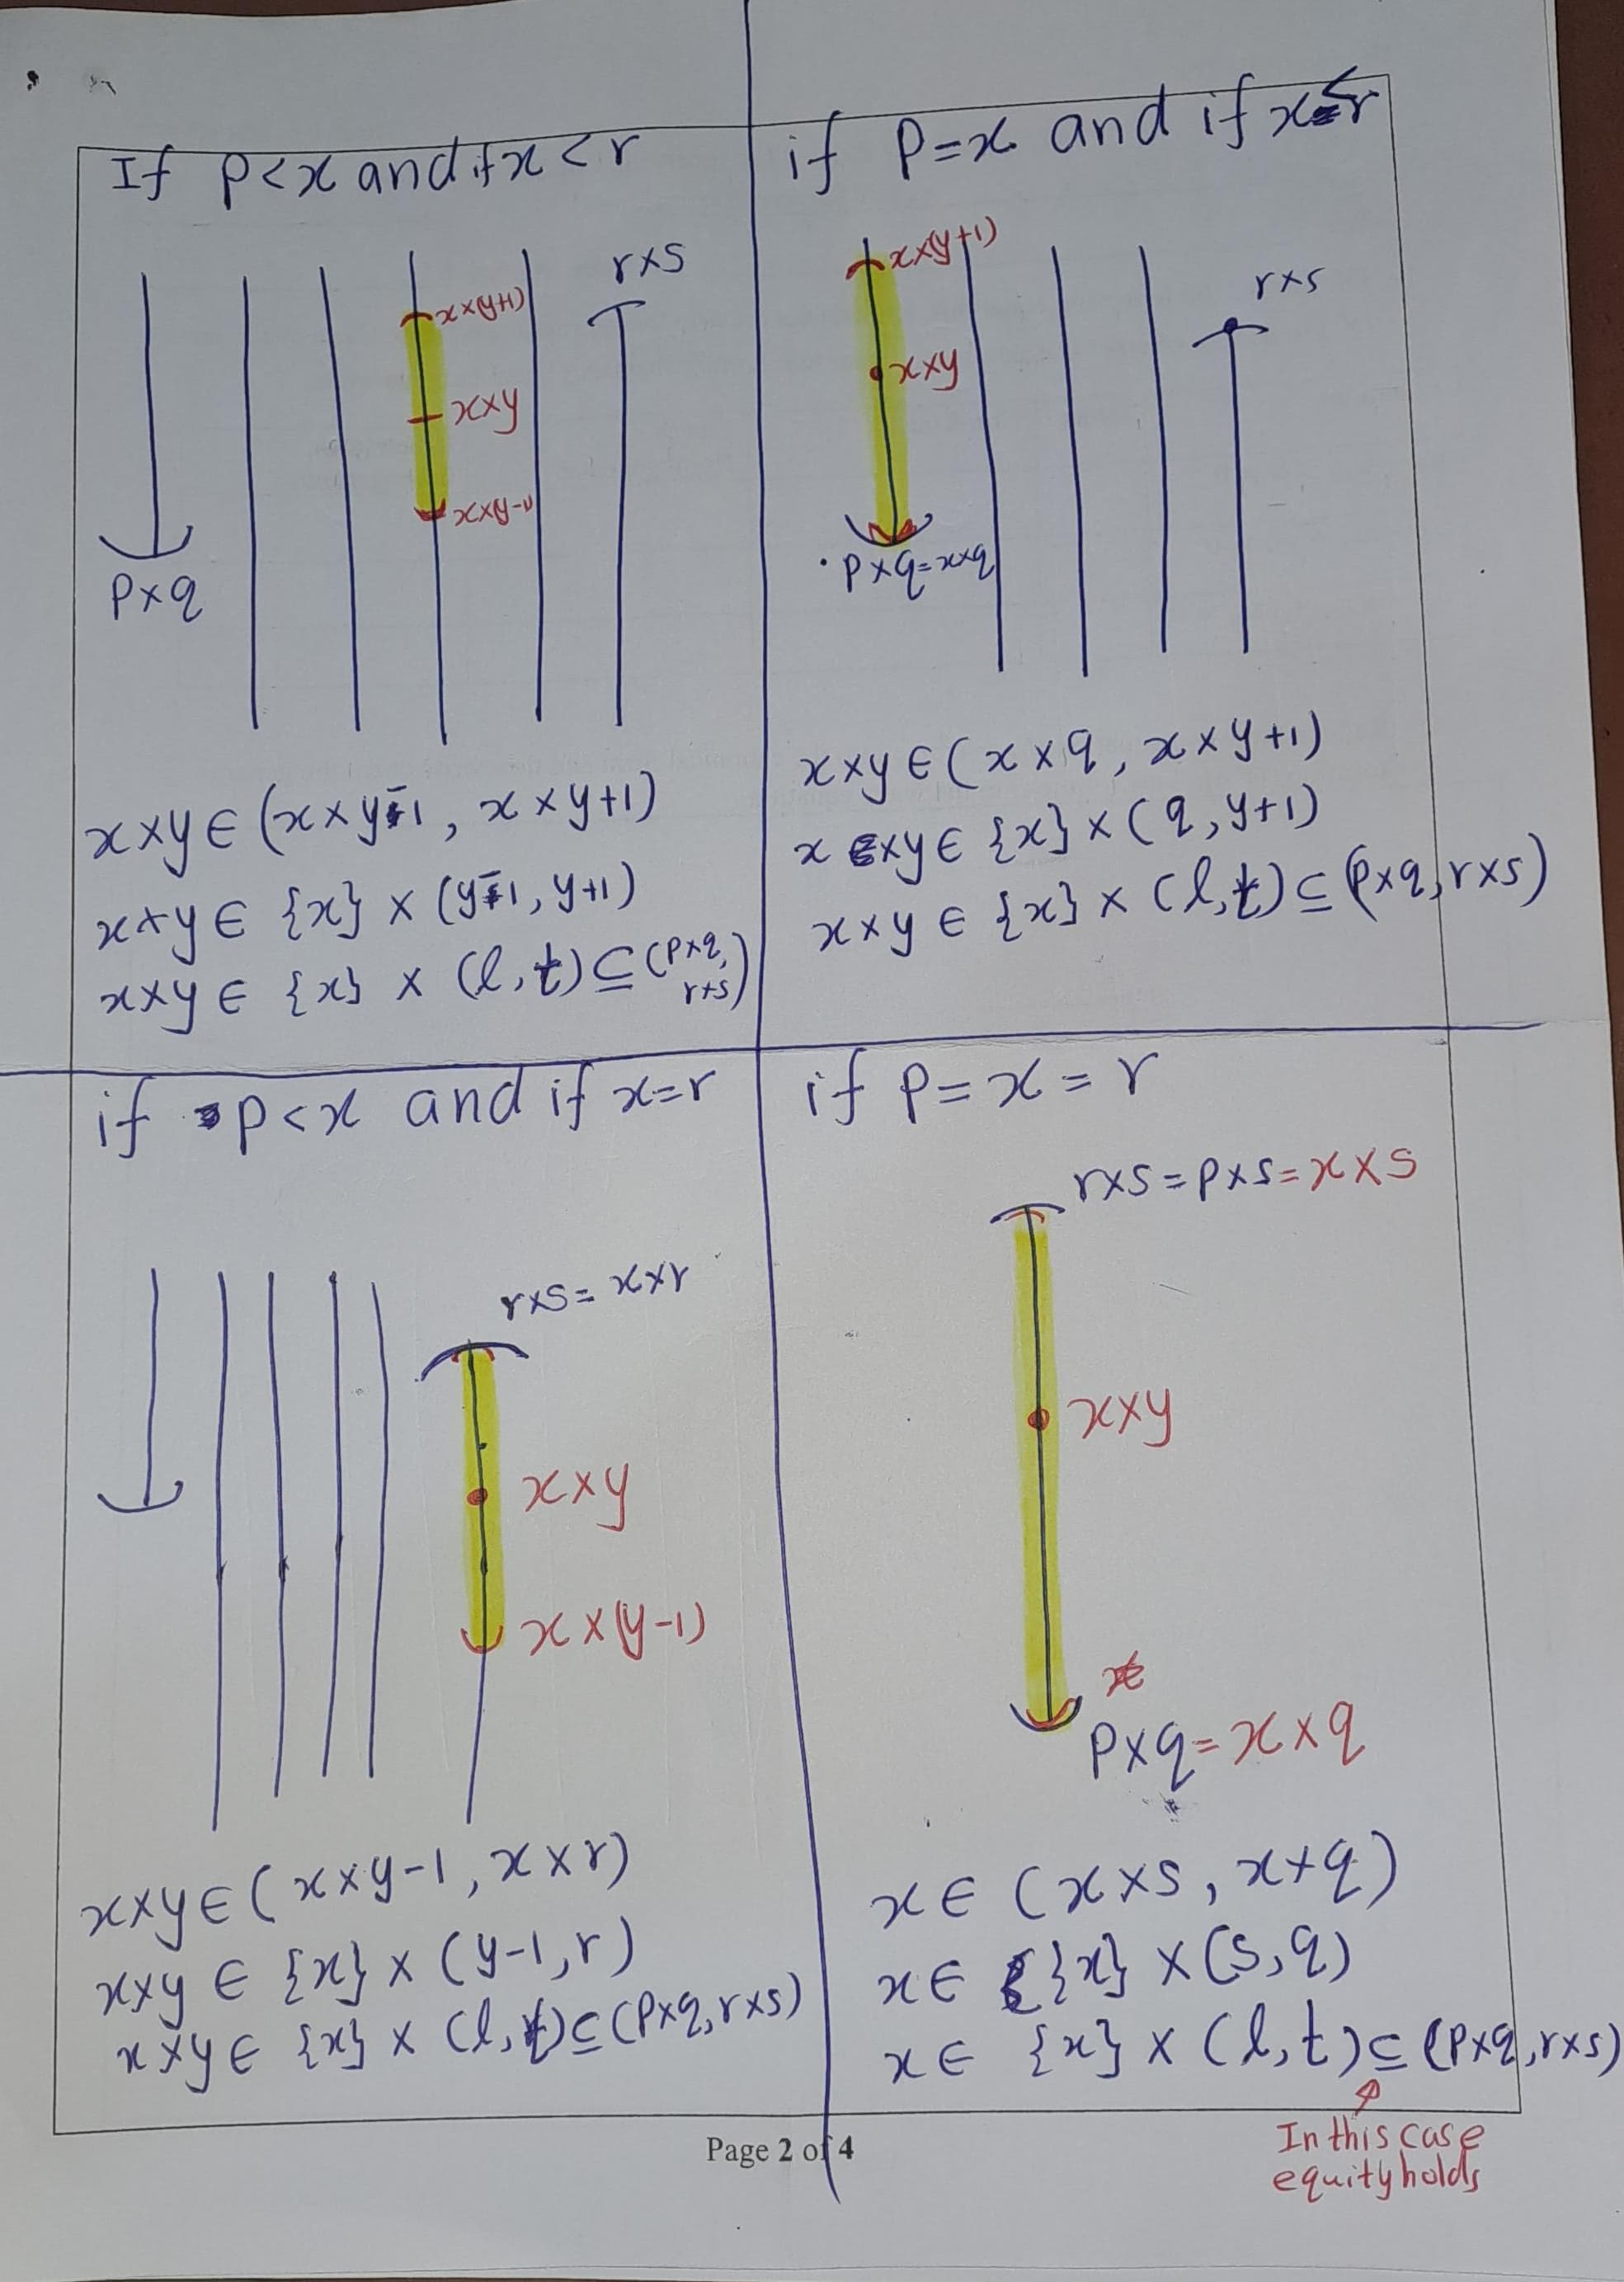
\includegraphics{figures/figure 12.jpg}
\caption{\label{fig:fig12}\(~\)}
\end{figure}

\begin{definition}
\protect\hypertarget{def:unnamed-chunk-42}{}\label{def:unnamed-chunk-42}Let \(\pi_1 : X \times Y \to X\) be defined by the equation
\(\pi_1(x, y) = x\);\\
and let \(\pi_2 : X \times Y \to Y\) be defined by the equation
\(\pi_2(x, y) = y\).

The maps \(\pi_1\) and \(\pi_2\) are called the \emph{projections} of \(X \times Y\) onto its first and second factors, respectively.
\end{definition}

\hypertarget{the-subspace-topology}{%
\section{The Subspace Topology}\label{the-subspace-topology}}

\emph{A subset of a topological space has a naturally induced topology, called the subspace topology. In geometry, the subspace topology is the source of all funky typologies.}

\begin{definition}
\protect\hypertarget{def:unnamed-chunk-43}{}\label{def:unnamed-chunk-43}Let \((X, \mathcal{T})\) be a topological space. Let \(Y\subseteq X\). The collection
\[\mathcal{T}_Y = \{Y \cap U | U \in \mathcal{T}\}\] is a topology on \(Y\), called the subspace topology.
\end{definition}

\begin{proof}

(Proof of the collection \(\mathcal{T}_Y\) is a tology).

\begin{itemize}
\tightlist
\item
  (T1) This is very easy to see. \(\mathcal{T}_Y\) contains \(\emptyset\) and \(Y\) because \(\emptyset = Y \cap \emptyset and Y = Y \cap X\), where \(\emptyset\) and \(X\) are elements of \(\mathcal{T}\).
\item
  (T2) Let \(\{U_\alpha \cap Y\in \mathcal{T_Y}:\alpha \in I, \text{ I is index set}\}\) be collection of open sets in subspace toplogy of \(Y\), where \(U_\alpha\in \mathcal{T}\).
  \[\bigcup_{\alpha \in I}\left(U_\alpha\cap Y\right)
    =\bigcup_{\alpha \in I}\left(U_\alpha\right)\cap Y.\]
  Thus it contains in \(\mathcal{T}\). Thus \(\mathcal{T}_Y\) is closed under arbitary unions.
\item
  (T3) Let \(U_1\cap Y, U_2\cap Y,..., U_n\cap Y\) be finite collection of open sets in subspace toplogy of \(Y\) in \(X\).
  \[(U_1\cap Y)\bigcap (U_2\cap Y)\bigcap \cdots \bigcap (U_n\cap Y)=(U_1\cap U_2 \cap \cdot U_n)\bigcap Y.\]
  Thus it contains in \(\mathcal{T}\).Thus \(\mathcal{T}_Y\) is closed under finite intersections.
\end{itemize}

\end{proof}

\begin{lemma}
\protect\hypertarget{lem:unnamed-chunk-45}{}\label{lem:unnamed-chunk-45}Let \((X, \mathcal{T})\) be a topological space, and \(Y\subseteq X\). If \(\mathcal{B}\) is a basis for \(\mathcal{T}\) then the collection
\[\mathcal{B}_Y = \{B \cap Y | B \in \mathcal{B}\}\]
is a basis for the subspace topology on \(Y\).
\end{lemma}

\begin{proof}
Let \(V\in \mathcal{T}_Y\). Then \(V=U\cap Y\) for some \(U\in \mathcal{T}\). For every \(x \in V\), there is \(B \in \mathcal{B}\) such that \(x \in B \subset U\) since \(\mathcal{B}\) is a basis of \(\mathcal{T}\) (Lemma \ref{lem:lemmaTequalsTB}). Now we found \(Y \cap B\) such that \(x \in Y \cap B \subset V\).
\end{proof}

\begin{figure}
\centering
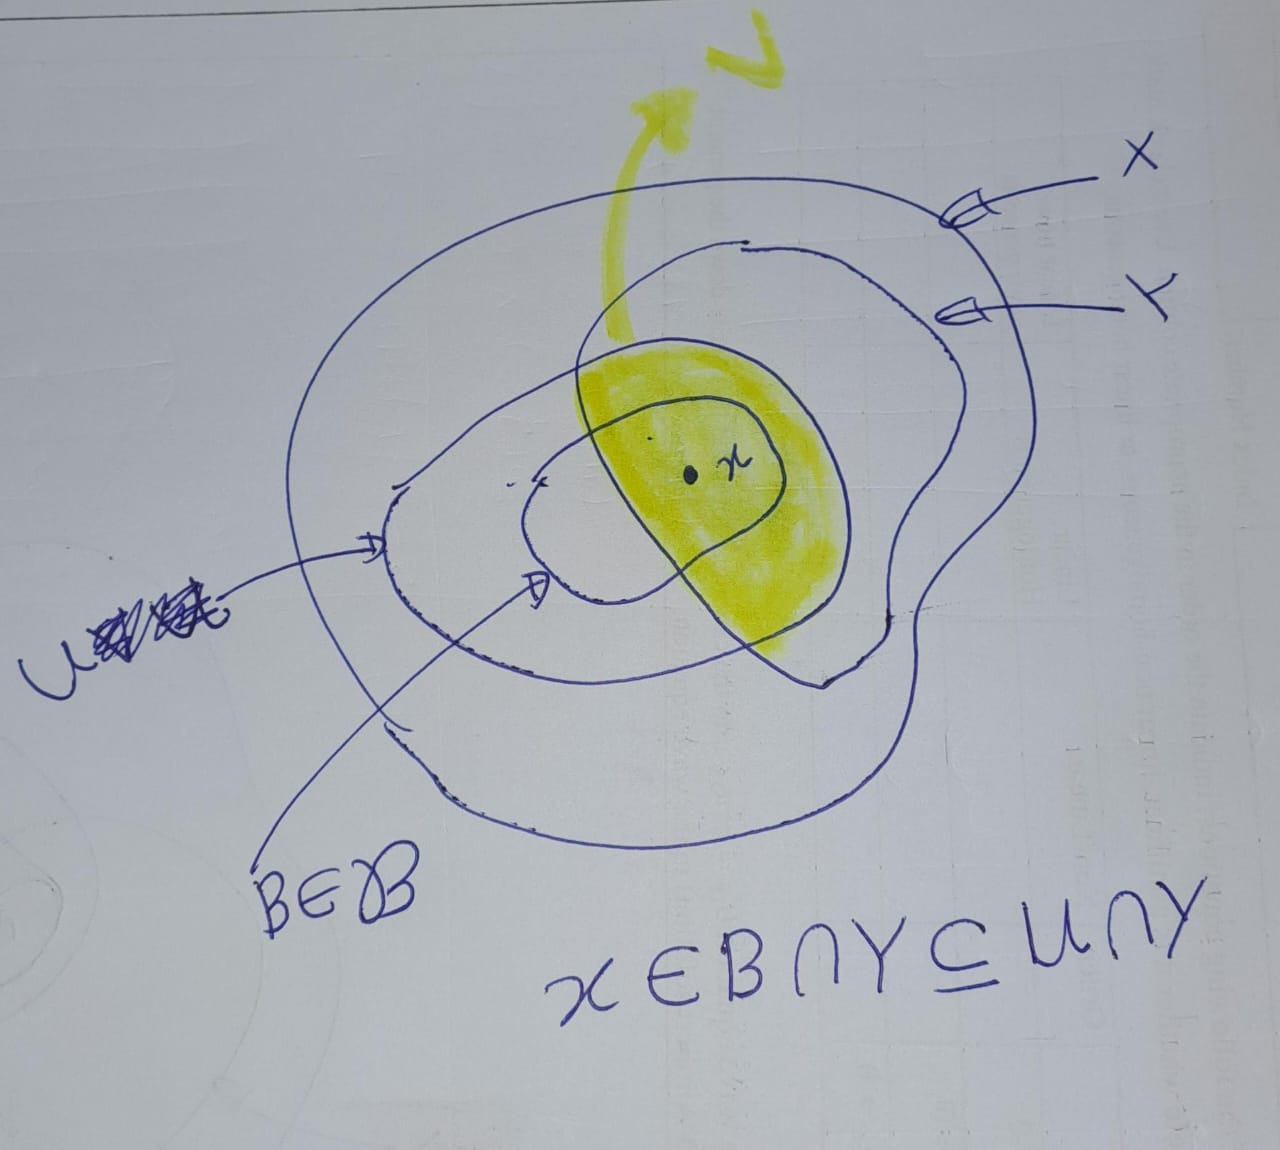
\includegraphics{figures/figure 13.jpg}
\caption{\label{fig:fig13}\(~\)}
\end{figure}

\begin{example}
\protect\hypertarget{exm:unnamed-chunk-47}{}\label{exm:unnamed-chunk-47}Let \(I = [0, 1]\). The dictionary order on \(I \times I\) is just the restriction to \(I \times I\) of the dictionary order on the plane \(\mathbb{R} \times \mathbb{R}\). However, the dictionary order topology on \(I \times I\) is \textbf{NOT} the same as the subspace topology on \(I \times I\) obtained from the dictionary order topology on \(\mathbb{R} \times \mathbb{R}\)!

For example, the set \(\{\frac{1}{2}\} \times (\frac{1}{2}, 1]\) is open in \(I \times I\) in the
subspace topology, but not in the order topology, as you can check.

See Figure \ref{fig:fig14}.
\end{example}

\begin{figure}
\centering
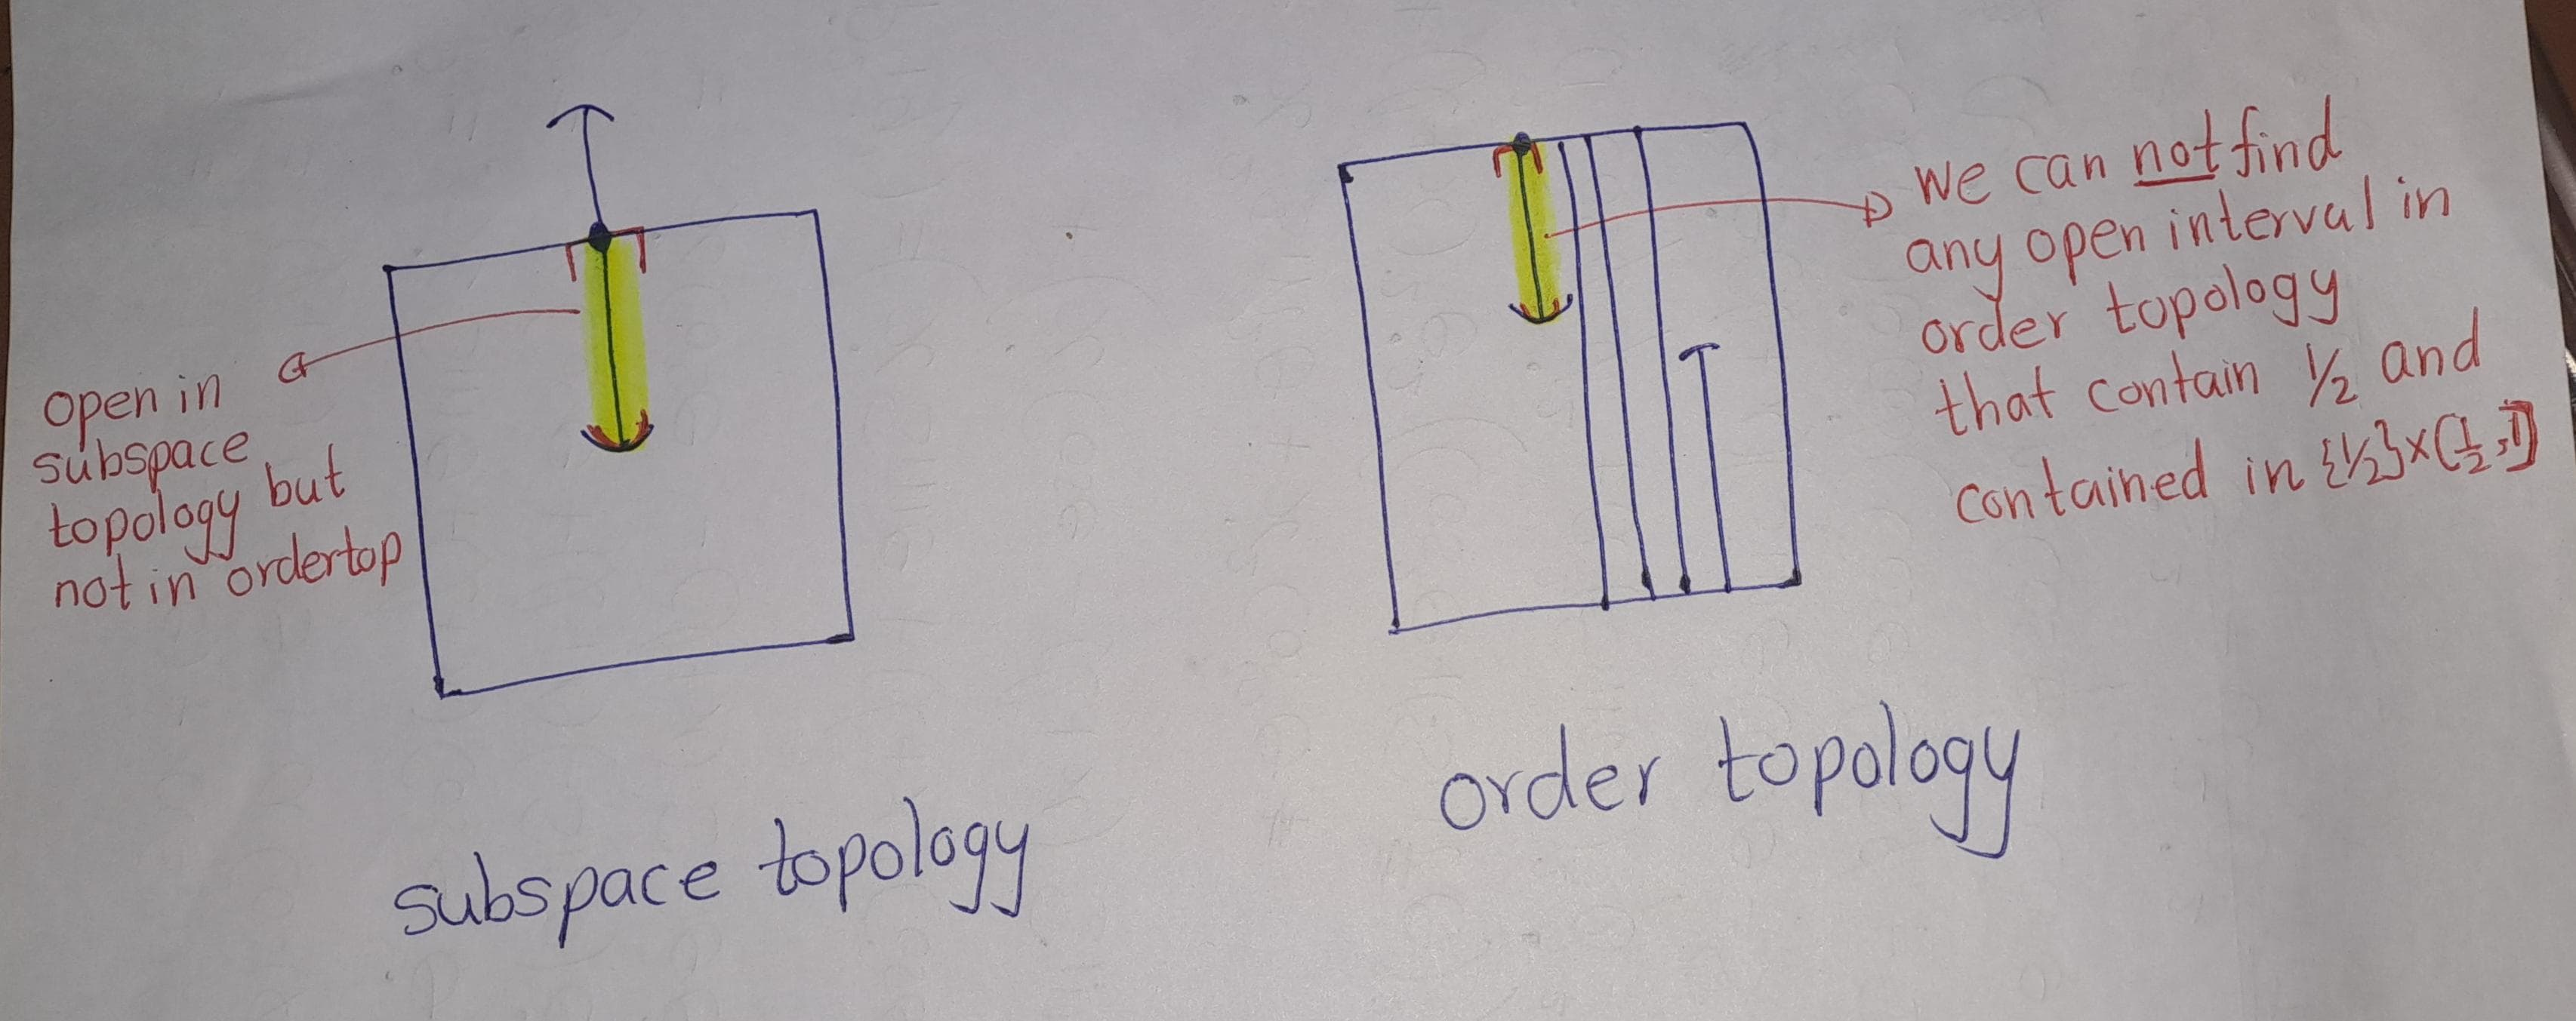
\includegraphics{figures/figure 14.jpg}
\caption{\label{fig:fig14}\(~\)}
\end{figure}

\textbf{Notation} : The set \(I \times I\) in the dictionary order topology will be called the ordered square, and denoted by \(I_o^2\).

Let's generalized the idea.

\begin{lemma}
\protect\hypertarget{lem:unnamed-chunk-48}{}\label{lem:unnamed-chunk-48}The subspace topology on \(I \times I\) obtained from the dictionary order topology on \(\mathbb{R} \times \mathbb{R}\) is strictly finer than the dictionary order toplogy on \(I \times I\).
\end{lemma}

\begin{proof}
So, as pervious we have to proove two things they are finer condtion and strictly condition.

Let \((a_1\times b_1, a_2 \times b_2)\) be a basis elemenet of order toplogy. and \(x\times y \in (a_1\times b_1, a_2 \times b_2)\)

\begin{itemize}
\item
  \textbf{Case I} \((a_1<x<a_2)\):
  \[x\times y \in (x\times-1,x\times 2)\cap I^2= [x\times 0,x\times 1]=\{x\}\times [0,1] \subset (a_1\times b_1, a_2 \times b_2)\]
  Note that \((x\times -1,x\times 2)\cap I^2\) is a basis element of subspace topology.
\item
  \textbf{Case II} \((a_1=x<a_2)\):
  \[x\times y \in (x\times b_1,x\times 2)\cap I^2= [x\times b_1,x\times 1]=\{x\}\times (b_1,1] \subset (a_1\times b_1, a_2 \times b_2)\]
  Note that \((x\times b_1,x\times 2)\cap I^2\) is a basis element of subspace topology.
\item
  \textbf{Case III} \((a_1<x=a_2)\):
  \[x\times y \in (x\times -1,x\times b_2)\cap I^2= [x\times 0,x\times b_2]=\{x\}\times [0,b_2) \subset (a_1\times b_1, a_2 \times b_2)\]
  Note that \((x\times -1,x\times b_2)\cap I^2\) is a basis element of subspace topology.
\item
  \textbf{Case IV} \((a_1=x=a_2)\):
  \[x\times y \in (x\times b_1,x\times b_2)\cap I^2= [x\times b_1,x\times b_2]=\{x\}\times [b_1,b_2) \subset (a_1\times b_1, a_2 \times b_2)\]
  Note that \((x\times b_1,x\times b_2)\cap I^2\) is a basis element of subspace topology.
\end{itemize}

See figure \ref{fig:fig15}

In above all four cases, we have found basis element of subspace topology that conatain \(x\times y\) and conatined in \((a_1\times b_1, a_2 \times b_2)\).
\end{proof}

\begin{figure}
\centering
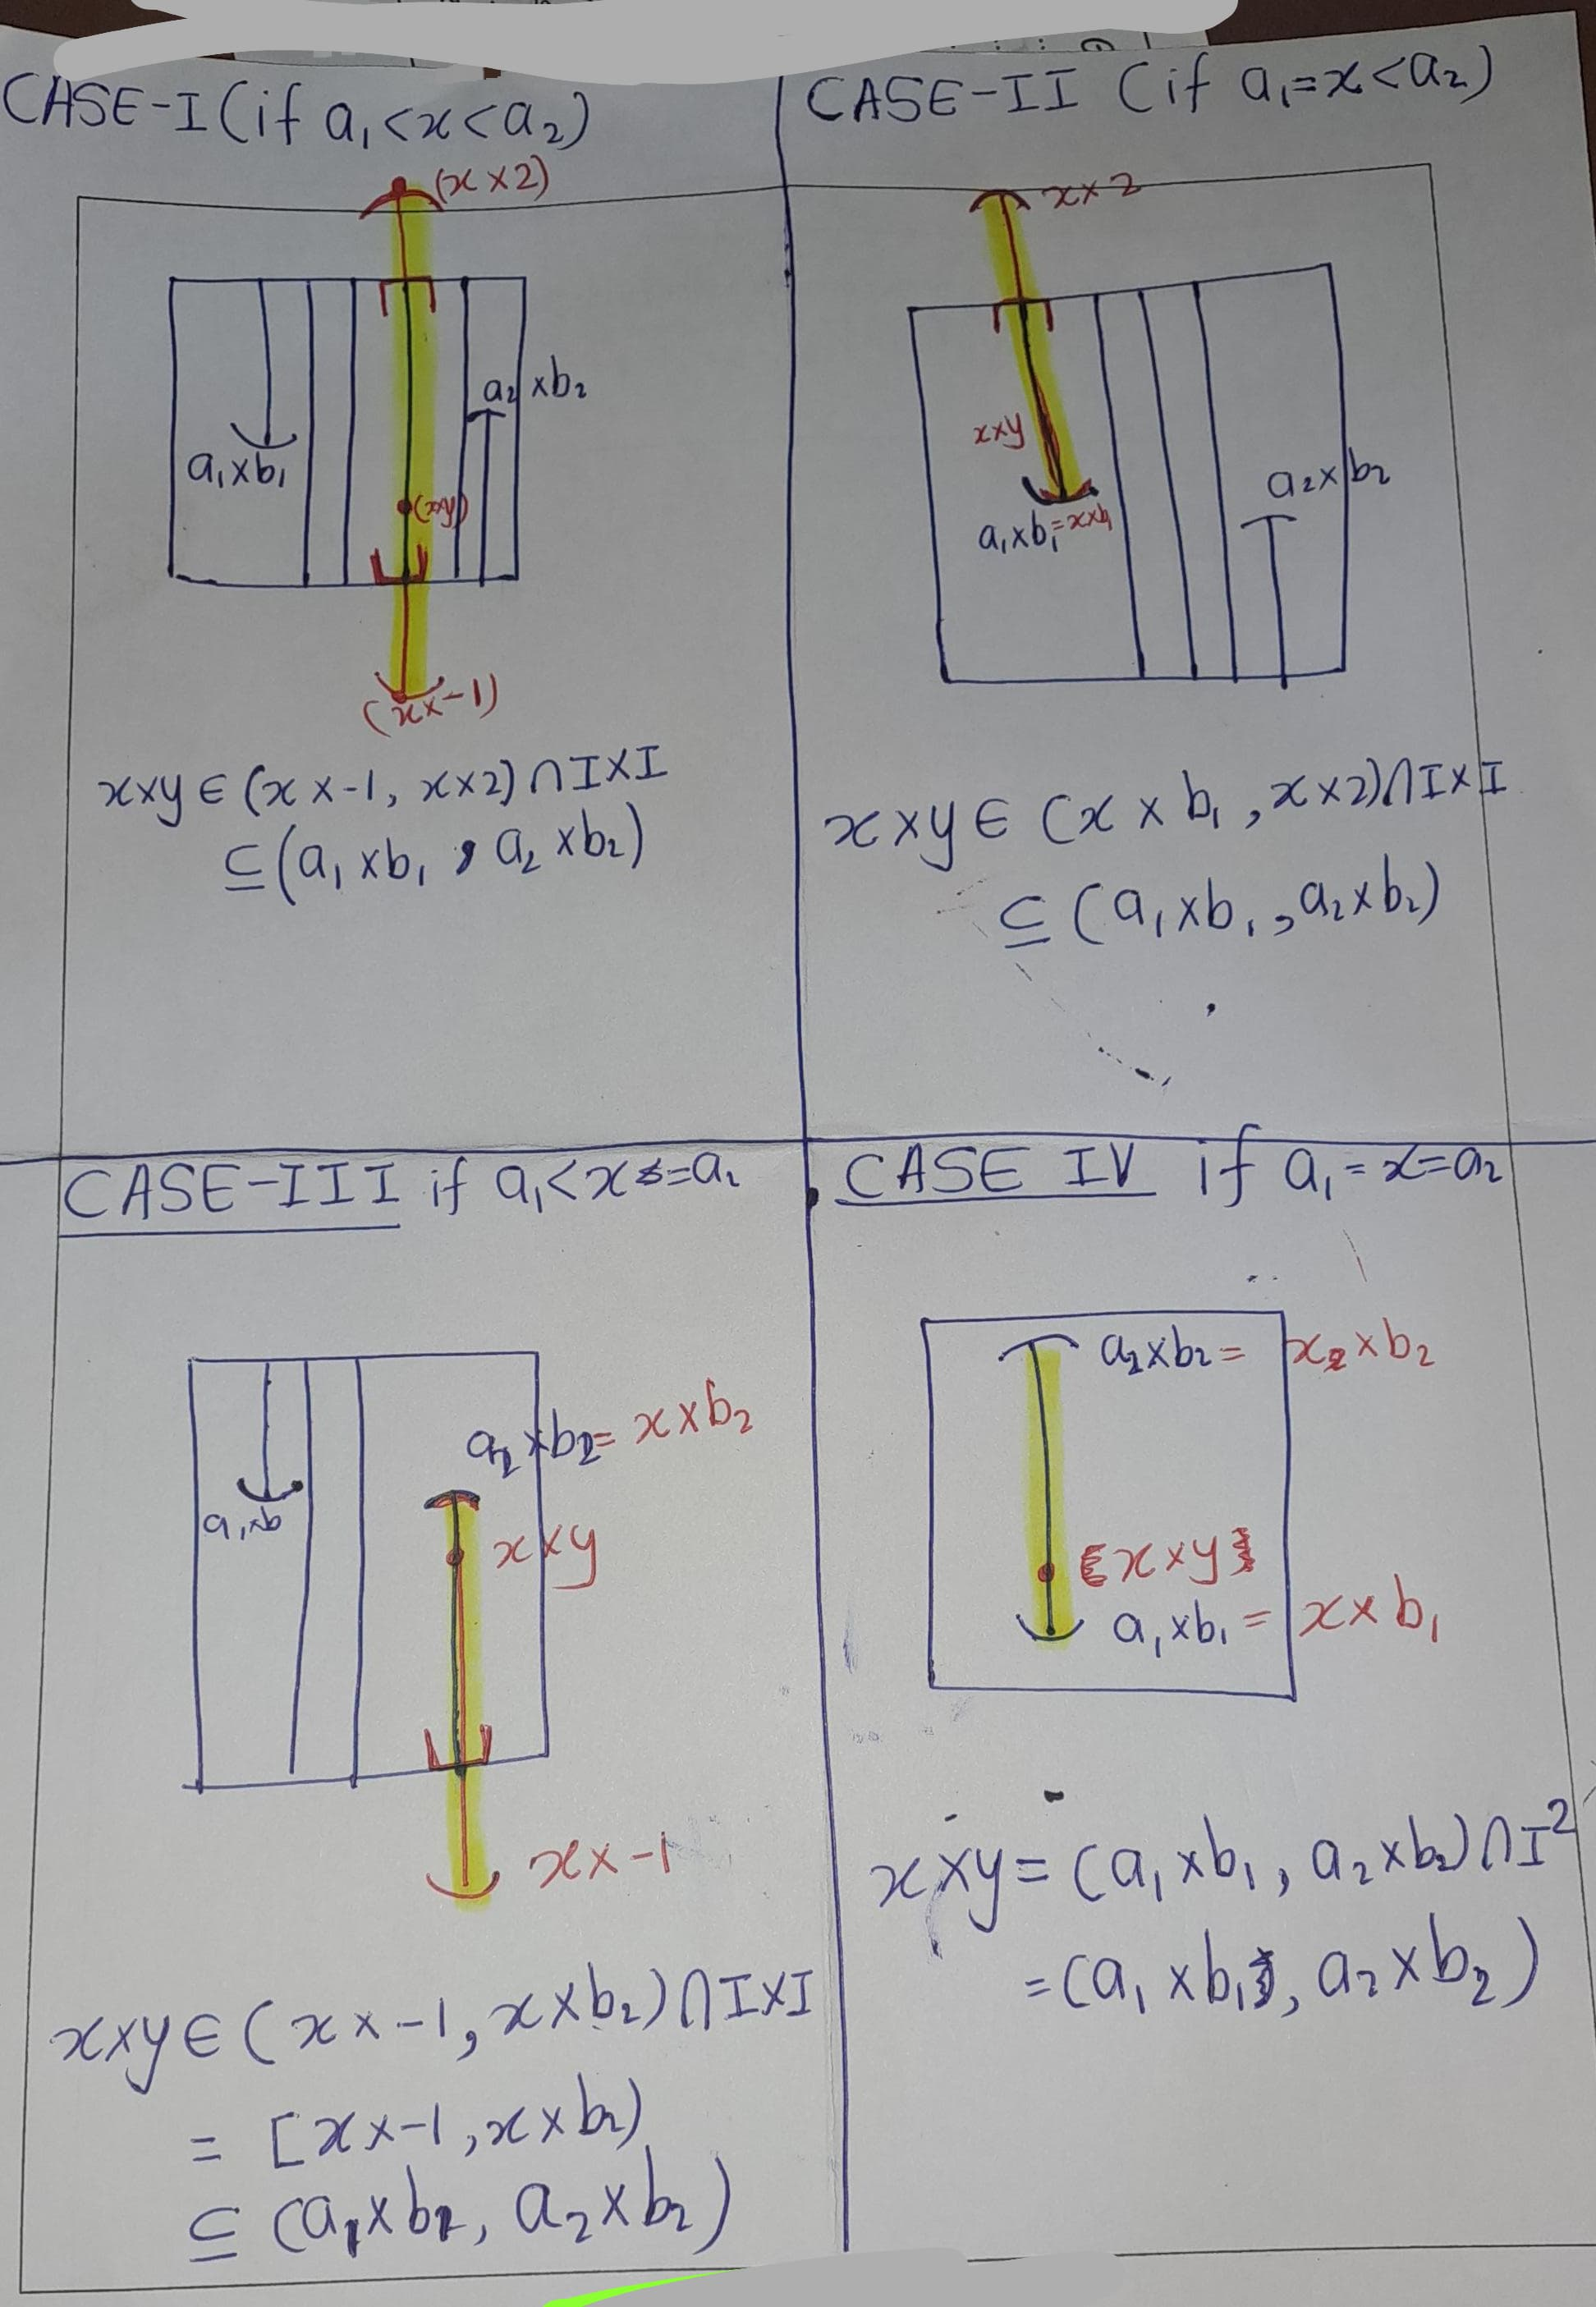
\includegraphics{figures/figure 15.jpg}
\caption{\label{fig:fig15}\(~\)}
\end{figure}

\hypertarget{closed-sets-and-limit-points}{%
\section{Closed Sets and Limit Points}\label{closed-sets-and-limit-points}}

Now that we have a few examples at hand, we can introduce some of the basic concepts associated with topological spaces. In this section, we treat the notions of closed set closure of a set, and limit point. These lead naturally to consideration of a certain axiom for topological spaces called the Hausdorff axiom.

\hypertarget{closed-set}{%
\subsection{Closed Set}\label{closed-set}}

\emph{Closed sets are nothing but complement of open sets. On the other hand, we can also say that open sets are nothing but complement of closed sets. Thus we can actually use closed sets to define topology, although mathematicians usually use open sets to define topology.}

\begin{definition}
\protect\hypertarget{def:unnamed-chunk-50}{}\label{def:unnamed-chunk-50}

Let \(A\) be a subset of a topological space \((X, \mathcal{})\).

\(A\) is a closed set of \(X\) if \(X\setminus A\) is an open set.

\begin{itemize}
\tightlist
\item
  The closure Cl\((A)=\overline{A}\) of \(A\) in \(X\) is the intersection of all closed sets of \(X\), containing \(A\).
  \[\text{Cl}(A)=\overline{A}=\bigcap \left\{C \text{ is closed in } X~ \&~  A \subset C\right\}\]
  The smallest closed set that containing\(A\) is the closure of \(A\).
\item
  The interior \(\text{Int}(A)=\mathring{A}\) of \(A\) in \(X\) is the union of all open sets of \(X\), contained in \(A\).
  \[\text{Int}(A)=\mathring{A}=\bigcup \left\{U \text{ is open in } X~ \&~  U \subset A\right\}\]
  The largest open set contanied in \(A\) is the interior of \(A\).
\item
  \(x \in X\) is a limit point (or ``cluster point,'' or ``point of accumulation'') of \(A\),
  if every neighborhood
  of \(x\) intersects \(A\) in some point other than \(x\) itself. In other words, \(x \in X\) is a limit point of \(A\), if \(x \in \overline{A\setminus\{x\}}\).
\end{itemize}

\end{definition}

\begin{remark}
\leavevmode

\begin{itemize}
\tightlist
\item
  \(\emptyset, X\) are closed.
\end{itemize}

\emph{I am not going to proove these things. I just give an idea.}
(This is trivial.)
- Fnite unions of closed sets are closed.
\[  \bigcup_{i=1}^n
    \underbrace{(X\setminus~ \underbrace{U_i}_{\text{open}})}_{\text{closed}}
    =X\setminus \underbrace{\bigcap_{i=1}^nU_i}_{\text{open}}\]
- Arbitrary intersection of closed sets are closed.
\[  \bigcap_{\alpha\in I}
    \underbrace{(X\setminus~ \underbrace{U_\alpha}_{\text{open}})}_{\text{closed}}
    =X\setminus \underbrace{\bigcup_{\alpha \in I} U_i}_{\text{open}}\]

\end{remark}

\begin{example}
\protect\hypertarget{exm:unnamed-chunk-52}{}\label{exm:unnamed-chunk-52}The subset \([a, b]\) of \(\mathbb{R}\) is closed because its complement
\[\mathbb{R}\setminus [a, b] = (−\infty, a) \cup (b, +\infty)\],
is open.
\end{example}

\begin{remark}
These facts justify our use of the terms ``closed interval'' and ``closed ray.'' The subset \([a, b)\) of \(\mathbb{R}\) is neither open nor closed.
\end{remark}

\begin{example}
\protect\hypertarget{exm:unnamed-chunk-54}{}\label{exm:unnamed-chunk-54}Similary,the subset \([a, +\infty)\) of \(\mathbb{R}\) is closed because its complement
\[\mathbb{R}\setminus [a, +\infty) = (−\infty, a) \],
is open.
\end{example}

\begin{example}
\protect\hypertarget{exm:unnamed-chunk-55}{}\label{exm:unnamed-chunk-55}In the plane \(\mathbb{R}^2\), the set
\[\{x \times y | x \geq 0 \text{ and }y ≥ 0\}\]
is closed, because its complement is the union of the two sets
\[(−\infty, 0) \times \mathbb{R} \text { and }\mathbb{R} \times (−\infty, 0),\]
each of which is a product of open sets of \(\mathbb{R}\) and is, therefore, open in \(\mathbb{R}^2\).
\end{example}

\begin{example}
\protect\hypertarget{exm:unnamed-chunk-56}{}\label{exm:unnamed-chunk-56}In the finite complement topology on a set \(X\), the closed sets consist of \(X\) itself and all finite subsets of \(X\).
\end{example}

\begin{example}
\protect\hypertarget{exm:unnamed-chunk-57}{}\label{exm:unnamed-chunk-57}In the discrete topology on the set \(X\), every set is open; it follows that every set is closed as well.
\end{example}

\begin{example}
\protect\hypertarget{exm:unnamed-chunk-58}{}\label{exm:unnamed-chunk-58}Consider the following subset of the real line:
\[Y = [0, 1] \cup (2, 3)\],
in the subspace topology. In this space,

The set \([0, 1]\) is open, since it is the intersection of the open set \((−\frac{1}{2} , \frac{3}{2} )\) of \(\mathbb{R}\) with \(Y\) . Similarly, \((2, 3)\) is open as a subset of \(Y\) ; it is even open as a subset of \(\mathbb{R}\). Since \([0, 1]\) and \((2, 3)\) are complements in \(Y\) of each other, we conclude that both \([0, 1]\) and \((2, 3)\) are closed as subsets of \(Y\).
\end{example}

\textbf{Fun Fact}: These examples suggest that an answer to the mathematician's riddle: ``How is a set different from a door?'' should be: ``A door must be either open or closed, and cannot be both, while a set can be open, or closed, or both, or neither!

The collection of closed subsets of a space X has properties similar to those satisfied by the collection of open subsets of \(X\);

\begin{theorem}
\protect\hypertarget{thm:unnamed-chunk-59}{}\label{thm:unnamed-chunk-59}

Let \(X\) be a topological space. Then the following conditions hold:

\begin{enumerate}
\def\labelenumi{(\arabic{enumi})}
\tightlist
\item
  \(\emptyset\) and \(X\) are closed.
\item
  Arbitrary intersections of closed sets are closed.
\item
  Finite unions of closed sets are closed.
\end{enumerate}

\end{theorem}

\begin{proof}
\leavevmode

\begin{enumerate}
\def\labelenumi{\arabic{enumi})}
\tightlist
\item
  \(\emptyset\) and \(X\) are closed because they are the complements of the open sets \(X\) and \(\emptyset\), respectively.
\item
  Given a collection of closed sets \(\{A_{\alpha}\}_{\alpha \in J}\), we apply DeMorgan's law, \[X \setminus \bigcup_{\alpha \in J} A_{\alpha} = \bigcap_{\alpha \in J} (X \setminus A_{\alpha})\]. Since the sets \(X \setminus A_{\alpha}\) are open by definition, the right side of this equation represents an arbitrary union of open sets, and is thus open. Therefore, \(\bigcup A_{\alpha}\) is closed.
\item
  Similarly, if \(A_i\) is closed for \(i = 1, \ldots, n\), consider the equation \[X \setminus \bigcap_{i=1}^{n} A_i = \bigcup_{i=1}^{n} (X \setminus A_i)\].
  The set on the right side of this equation is a finite intersection of open sets. Hence \(\bigcup A_i\) is closed.
\end{enumerate}

\end{proof}

Instead of using open sets, one could just as well specify a topology on a space by giving a collection of sets (to be called ``closed sets'') satisfying the three properties of this theorem. One could then define open sets as the complements of closed sets and proceed just as before. This procedure has no particular advantage over the one we have adopted, and most mathematicians prefer to use open sets to define topologies.

Now when dealing with subspaces, one needs to be careful in using the term ``closed set.'' If \(Y\) is a subspace of \(X\), we say that a set \(A\) is closed in \(Y\) if \(A\) is a subset of \(Y\) and if \(A\) is closed in the subspace topology of \(Y\) (that is, if \(Y \setminus A\) is open in \(Y\) ). We have the following theorem:

\begin{theorem}
\protect\hypertarget{thm:qw}{}\label{thm:qw}Let \(X\) be a toplogical space and \(Y\) is a subspace of \(X\), and \(A\) is a subset of \(Y\) , then \(A\) is closed \(\iff ~A=Y \cap C\) forsome \(C\) is closed in \(X\).
\end{theorem}

\begin{proof}
\leavevmode

\begin{itemize}
\tightlist
\item
  (\(\Longleftarrow\)) Suppose that \(A=Y \cap C\) for some closed set \(C\) in \(X\). (See Figure \ref{fig:fig19} Thus, \(X\setminus C\) is open in \(X\). So, \((X\setminus C)\cap Y\) is open in \(Y\), by definition of the subspace topology. But,
  \[(X\setminus C)\cap Y=Y\setminus (C\cap Y)=Y\setminus A.\]
  . Hence \(Y \setminus A\) is open in \(Y\).Therfore, \(A\) is closed in \(Y\).
\item
  (\(\Longrightarrow\)) Now Suppose that \(A\) is closed in \(Y\). (See Figure \ref{fig:fig20} Then, \(Y\setminus A\) is open in \(Y\). Thus by definition, \(Y\setminus A= U \cap Y\), forsome open set \(U\) in \(X\). So, \(X\setminus U\) is closed in \(X\). Now consider,
  \[Y \cap (X\setminus U)=Y\setminus (Y \cap U)=Y\setminus (Y \setminus U)=A.\]
  Thefore, \(Y \cap C\) forsome \(C\) is closed in \(X\).
\end{itemize}

\end{proof}

\begin{figure}
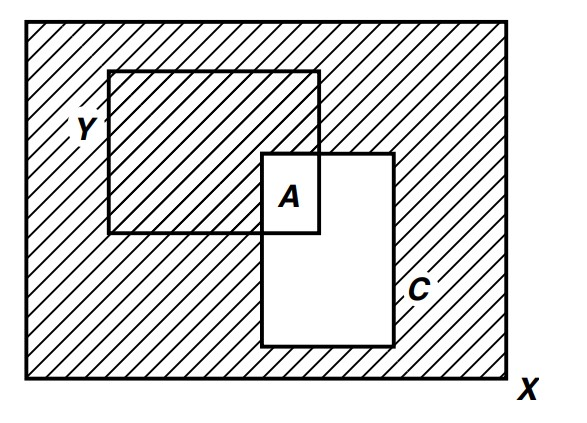
\includegraphics[width=0.5\linewidth]{figures/figure 19} \caption{$~$}\label{fig:fig19}
\end{figure}

\begin{figure}
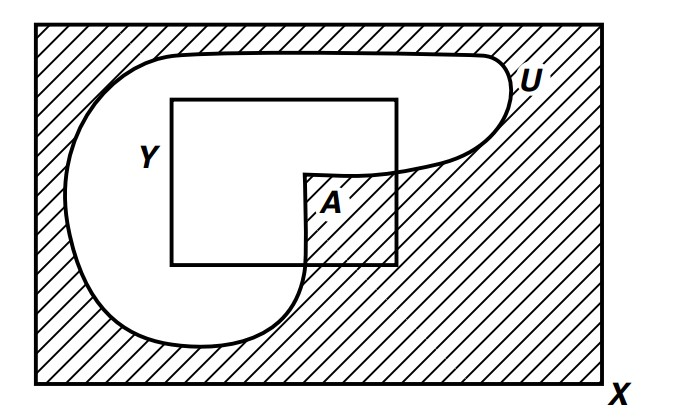
\includegraphics[width=0.5\linewidth]{figures/figure 20} \caption{$~$}\label{fig:fig20}
\end{figure}

\begin{remark}
A set \(A\) that is closed in the subspace \(Y\) may or may not be closed in the larger space \(X\).
\end{remark}

\begin{theorem}
\protect\hypertarget{thm:unnamed-chunk-63}{}\label{thm:unnamed-chunk-63}Let \(Y\) be a subspace of \(X\). If \(A\) is closed in \(Y\) and \(Y\) is closed in \(X\), then \(A\) is closed in \(X\).
\end{theorem}

\begin{proof}
Since \(Y\) is subspace in \(X\) and \(A\) is closed in \(Y\), by theorm \ref{thm:qw}, then there exist closed set \(C\) in \(X\) such that \[A=Y\cap C\]
Since, \(Y\) is closed in \(X\) and \(X\) is toplogical space, \(A=Y\cap C\) is closed in \(X\).
\end{proof}

\hypertarget{closure-and-interior-of-a-set}{%
\subsection{Closure and Interior of a Set}\label{closure-and-interior-of-a-set}}

\begin{definition}
\protect\hypertarget{def:unnamed-chunk-65}{}\label{def:unnamed-chunk-65}

Let \(A\) be a subset of a topological space \((X, \mathcal{})\).

\begin{itemize}
\tightlist
\item
  The closure Cl\((A)=\overline{A}\) of \(A\) in \(X\) is the intersection of all closed sets of \(X\), containing \(A\).
  \[\text{Cl}(A)=\overline{A}=\bigcap \left\{C \text{ is closed in } X~ \&~  A \subset C\right\}\]
  The smallest closed set that containing\(A\) is the closure of \(A\).
\item
  The interior \(\text{Int}(A)=\mathring{A}\) of \(A\) in \(X\) is the union of all open sets of \(X\), contained in \(A\).
  \[\text{Int}(A)=\mathring{A}=\bigcup \left\{U \text{ is open in } X~ \&~  U \subset A\right\}\]
  The largest open set contanied in \(A\) is the interior of \(A\).
\end{itemize}

\end{definition}

Obviously \(\text{Int}(A)\) is an open set and \(\overline{A}\) is a closed set; furthermore,
\[\text{Int}(A) \subseteq A \subseteq \overline{A}\]

\begin{lemma}
\protect\hypertarget{lem:unnamed-chunk-66}{}\label{lem:unnamed-chunk-66}Let \(Y\) be a subspace of \(X\) and \(A\subset Y\). Let \(\bar{A}\) denote the closure of \(A\) in \(X\). Then the closure of \(A\) in \(Y\) equals \(\bar{A} \cap Y\).
\end{lemma}

\begin{proof}
Let \(B\) denote the closure of \(A\) in \(Y\).

\begin{itemize}
\tightlist
\item
  \textbf{Claim}: \(B \subseteq \bar{A}\cap Y\)
\end{itemize}

The set \(\bar{A}\) is closed in \(X\), so \(\bar{A} \cap Y\) is closed in \(Y\) (By lemma \ref{thm:qw}). Since \(A\subset \bar{A}\cap Y\)(Since, \(\bar{A}\) is the smallest subset that conatin \(A\), and \(A\subseteq Y\)), and since by definition \(B\) equals the intersection of all closed subsets of \(Y\) containing \(A\), we must have \(B \subseteq (\bar{A} \cap Y)\).

\begin{itemize}
\tightlist
\item
  \textbf{Case-II}: \(\bar{A}\cap Y \subseteq B\)
\end{itemize}

we know that \(B\) is closed in \(Y\). Hence by lemma \ref{thm:qw}, \(B = C \cap Y\) for some set \(C\) closed in \(X\). Then \(C\) is a closed set of \(X\) containing \(A\); because \(\bar{A}\) is the intersection of all such closed sets, we conclude that \(\bar{A} \subseteq C\). Then
\((\bar{A}\cap Y ) \subset (C \cap Y ) = B\).
\end{proof}

\textbf{Terminology} : We shorten the statement to ``\(U\) is an open set containing \(x\)'' to the phrase ``\textbf{\(U\) is a neighbourhood of \(x\)}.

\begin{proposition}
\protect\hypertarget{prp:prop1}{}\label{prp:prop1}

Let \(A\) be a subset of the topological space \(X\).

\begin{enumerate}
\def\labelenumi{\alph{enumi})}
\item
  Then \(x \in \bar{A}\) if and only if every neighborhood \(U\) of \(x\) intersects \(A\). (has non-empty intersection with \(A\).)
\item
  Let \(\mathcal{B}\) be a basis for \(X\) , then \(x \in \bar{A}\) if and only if \(B\in \mathcal{B}\) which containing \(x\) intersects \(A\).
\end{enumerate}

\end{proposition}

\begin{proof}
\leavevmode

\begin{itemize}
\tightlist
\item
  Statemet a)

  \begin{itemize}
  \tightlist
  \item
    (\(\Longrightarrow\)): We are going to use indirect proof. Assume that \(x\in \bar{A}\). Then \(U=X\setminus \bar{A}\) is neighbohood of \(x\) which does not intersect \(A\) (\(\bar{A} \cap U=\emptyset\)). Since, \(A\subset \bar{A}\), then \(A \cup U =\emptyset\).
  \item
    (\(\Longleftarrow\)):
    Let \(U\) be a neighborhood of \(x\) which does not intersect \(A\). So, \(X\setminus U\) is closed and \(A\subset X\setminus U\), then \(\bar{A}\subset X\setminus U\). (because \$\textbackslash bar\{A\} is the smallest closed set that containing \(A\).So, \(x\in \bar{A}\)).
  \end{itemize}
\item
  Statemet b)

  \begin{itemize}
  \item
    \((\Longleftarrow)\): If every open set containing \(x\) intersects \(A\), so does
    every basis element \(B\) containing \(x\), because \(B\) is an open set.
  \item
    \((\Longrightarrow)\) if every
    basis element containing \(x\) intersects \(A\), so does every open set \(U\) containing \(x\), because \(U\) contains a basis element that contains \(x\).
  \end{itemize}
\end{itemize}

\end{proof}

\begin{example}
\protect\hypertarget{exm:e1}{}\label{exm:e1}

Let \(X\) be the real line \(\mathbb{R}\).

\begin{itemize}
\tightlist
\item
  If \(A = (0, 1]\), then \(\overline{A} = [0, 1]\), for every neighbourhood of 0 intersects \(A\), while every point outside \([0, 1]\) has a neighbourhood disjoint from \(A\).
\end{itemize}

Similar arguments apply to the following subsets of \(X\),

\begin{itemize}
\item
  If \(B = \left\{\frac{1}{n} | n \in \mathbb{Z}^{+}\right\}\), then \(\overline{B} = \{0\} \cup B\).
\item
  If \(C = \{0\} \cup (1, 2)\), then \(\overline{C} = \{0\}\cup[1, 2]\).
\item
  If \(\mathbb{Q}\) is the set of rational numbers, then \(\overline{\mathbb{Q}} = \mathbb{R}\).
\item
  If \(\mathbb{Z}^{+}\) is the set of positive integers, then \(\overline{\mathbb{Z}^{+}} = \mathbb{Z}^{+}\).
\item
  If \(\mathbb{R}^{+}\) is the set of positive reals, then the closure of \(\mathbb{R}^{+}\) is the set \(\mathbb{R}^{+} \cup \{0\}\).
\end{itemize}

\end{example}

\begin{example}
\protect\hypertarget{exm:unnamed-chunk-69}{}\label{exm:unnamed-chunk-69}Consider the subspace \(Y = (0, 1]\) of the real line \(\mathbb{R}\). The set \(A = \left(0, \frac{1}{2}\right)\) is a subset of \(Y\); its closure in \(\mathbb{R}\) is the set \(\left[0, \frac{1}{2}\right]\), and its closure in \(Y\) is the set \(\left[0, \frac{1}{2}\right] \cap Y = \left(0, \frac{1}{2}\right]\).
\end{example}

\hypertarget{limit-points}{%
\subsection{Limit Points}\label{limit-points}}

There is yet another way of describing the closure of a set, a way that involves the important concept of limit point, which we consider now.

\begin{definition}[Limit Point]
\protect\hypertarget{def:unnamed-chunk-70}{}\label{def:unnamed-chunk-70}If \(A\) is a subset of the topological space \(X\) and if \(x\) is a point of \(X\), we say that \(x\) is a limit point (or ``cluster point,'' or ``point of accumulation'') of \(A\) if every neighborhood of \(x\) intersects \(A\) in some point other than \(x\) itself.

Said differently, \(x\) is a limit point of \(A\) if it belongs to the closure of \(A \setminus \{x\}\). The point \(x\) may lie in \(A\) or not; for this definition it does not matter.
\end{definition}

\textbf{Notation}: let \(A^\prime\) be the set of all limit points of \(A\).

\begin{example}
\protect\hypertarget{exm:e2}{}\label{exm:e2}

Consider the real line \(\mathbb{R}\).

\begin{itemize}
\item
  If \(A = (0, 1]\), then the point 0 is a limit point of \(A\) and so is the point \(\frac{1}{2}\). In fact, every point of the interval \([0, 1]\) is a limit point of \(A\), but no other point of \(\mathbb{R}\) is a limit point of \(A\).
\item
  If \(B = \left\{\frac{1}{n} | n \in \mathbb{Z}^{+}\right\}\), then 0 is the only limit point of \(B\). Every other point \(x\) of \(\mathbb{R}\) has a neighborhood that either does not intersect \(B\) at all, or it intersects \(B\) only in the point \(x\) itself.
\item
  If \(C = \{0\} \cup (1, 2)\), then the limit points of \(C\) are the points of the interval \([1, 2]\).
\item
  If \(\mathbb{Q}\) is the set of rational numbers, every point of \(\mathbb{R}\) is a limit point of \(\mathbb{Q}\).
\item
  If \(\mathbb{Z}^{+}\) is the set of positive integers, no point of \(\mathbb{R}\) is a limit point of \(\mathbb{Z}^{+}\).
\item
  If \(\mathbb{R}^{+}\) is the set of positive reals, then every point of \(\{0\} \cup \mathbb{R}^{+}\) is a limit point of \(\mathbb{R}^{+}\).
\end{itemize}

\end{example}

Comparison of Examples \ref{exm:e1} and \ref{exm:e2} suggests a relationship between the closure of a
set and the limit points of a set. That relationship is given in the following theorem:

\begin{theorem}
\protect\hypertarget{thm:unnamed-chunk-71}{}\label{thm:unnamed-chunk-71}Let A be a subset of the topological space \(X\); let \(A^\prime\) be the set of all limit points of \(A\). Then \[\bar{A} = A \cup A^\prime\].
\end{theorem}

\begin{proof}
\leavevmode

\begin{itemize}
\item
  \textbf{Claim 1}: \(A^{\prime}\subseteq \bar{A}\)\\
  Supoose that \(x\in A^{\prime}\). Every neighborhood of \(x\) intersects \(A\) (in a point different from \(x\)). Therefore, by propostion \ref{prp:prop1}, \(x\) belongs to \(\overline{A}\). Hence \(A^{\prime} \subseteq \overline{A}\).
\item
  \textbf{Claim 2}: \(A \cup A^{\prime} \subseteq \overline{A}\).\\
  Since by definition \(A \subseteq \overline{A}\), it follows that \(A \cup A^{\prime} \subseteq \overline{A}\).
\item
  \textbf{Claim 3}:\(A \cup A^{\prime}\supseteq \overline{A}\).\\
  Let \(x\in \overline{A}\).

  \begin{itemize}
  \tightlist
  \item
    Case I: If \(x\in A\) then noting to proove.
  \item
    Case II: If \(x\not\in A\). Since \(x \in \overline{A}\), we know that every neighborhood \(U\) of \(x\) intersects \(A\); because \(x \notin A\), the set \(U\) must intersect \(A\) in a point different from \(x\). Then \(x \in A^{\prime}\), so that \(x \in A \cup A^{\circ}\), as desired.
  \end{itemize}
\end{itemize}

\end{proof}

\begin{corollary}
\protect\hypertarget{cor:unnamed-chunk-73}{}\label{cor:unnamed-chunk-73}A subset of a topological space is closed if and only if it contains all its limit points.
\end{corollary}

\begin{proof}
The set \(A\) is closed if and only if \(A = \overline{A}\), and the latter holds if and only if \(A^{\prime} \subset A\).
\end{proof}

\hypertarget{boundary-points}{%
\subsection{Boundary Points}\label{boundary-points}}

\begin{definition}
\protect\hypertarget{def:unnamed-chunk-75}{}\label{def:unnamed-chunk-75}If \(A \subset X\), we define the boundary of \(A\) by the equation
\[\text{Bd} \, A = \overline{A} \cap \overline{(X - A)}.\]
\end{definition}

\hypertarget{hausdorff-spaces}{%
\subsection{Hausdorff Spaces}\label{hausdorff-spaces}}

\begin{definition}
\protect\hypertarget{def:unnamed-chunk-76}{}\label{def:unnamed-chunk-76}A topological space \((X,\mathcal{T})\) is called a Hausdorff space if\\
(H1) \(\forall x,y \in X\) such that \(x \neq y\), \(\exists U_x, U_y \in \mathcal{T}\) such that \(x \in U_x\), \(y \in U_y\), and \(U_x \cap U_y = \emptyset\).

i.e., for every pair of distinct points \(x, y\) in \(X\), there are disjoint neighborhoods \(U_x\) and \(U_y\) of \(x\) and \(y\) respectively.
\end{definition}

\begin{figure}
\centering
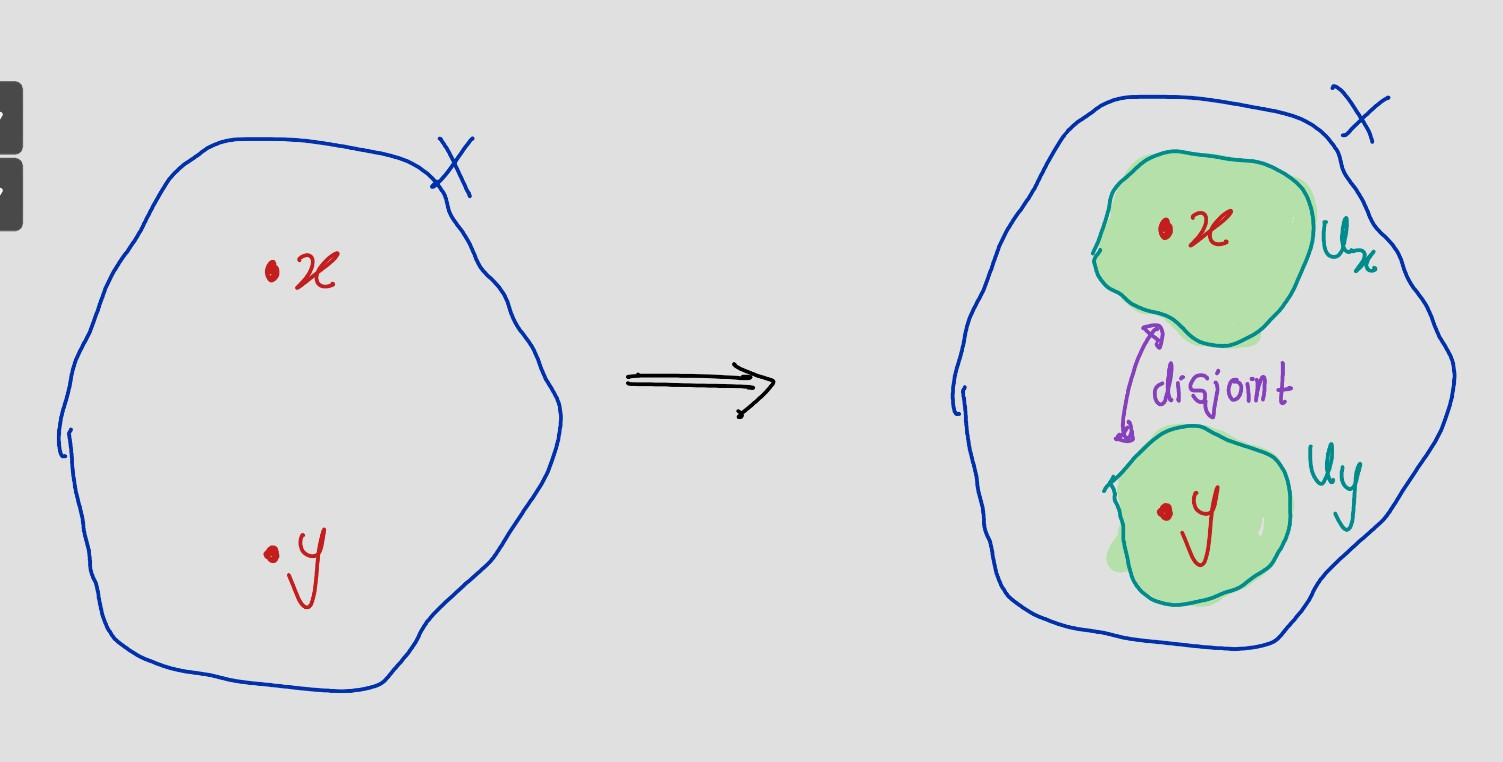
\includegraphics{figures/figure 16.jpg}
\caption{\label{fig:fig16}\(~\)}
\end{figure}

We called Hausdorff condition as \(T_2\) axiom. So Let's see another definition

\begin{figure}
\centering
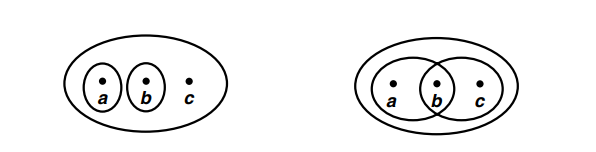
\includegraphics{figures/figure 02.png}
\caption{\label{fig:fig02}\(~\)}
\end{figure}

\begin{definition}
\protect\hypertarget{def:unnamed-chunk-77}{}\label{def:unnamed-chunk-77}A space \(X\) is a \emph{T1 space} if and only if it satisfies the following condition: For each \(x, y \in X\) such that \(x \neq y\), there exists an open set \(U \subset X\) such that \(x \in U\) but \(y \notin U\).
\end{definition}

\begin{figure}
\centering
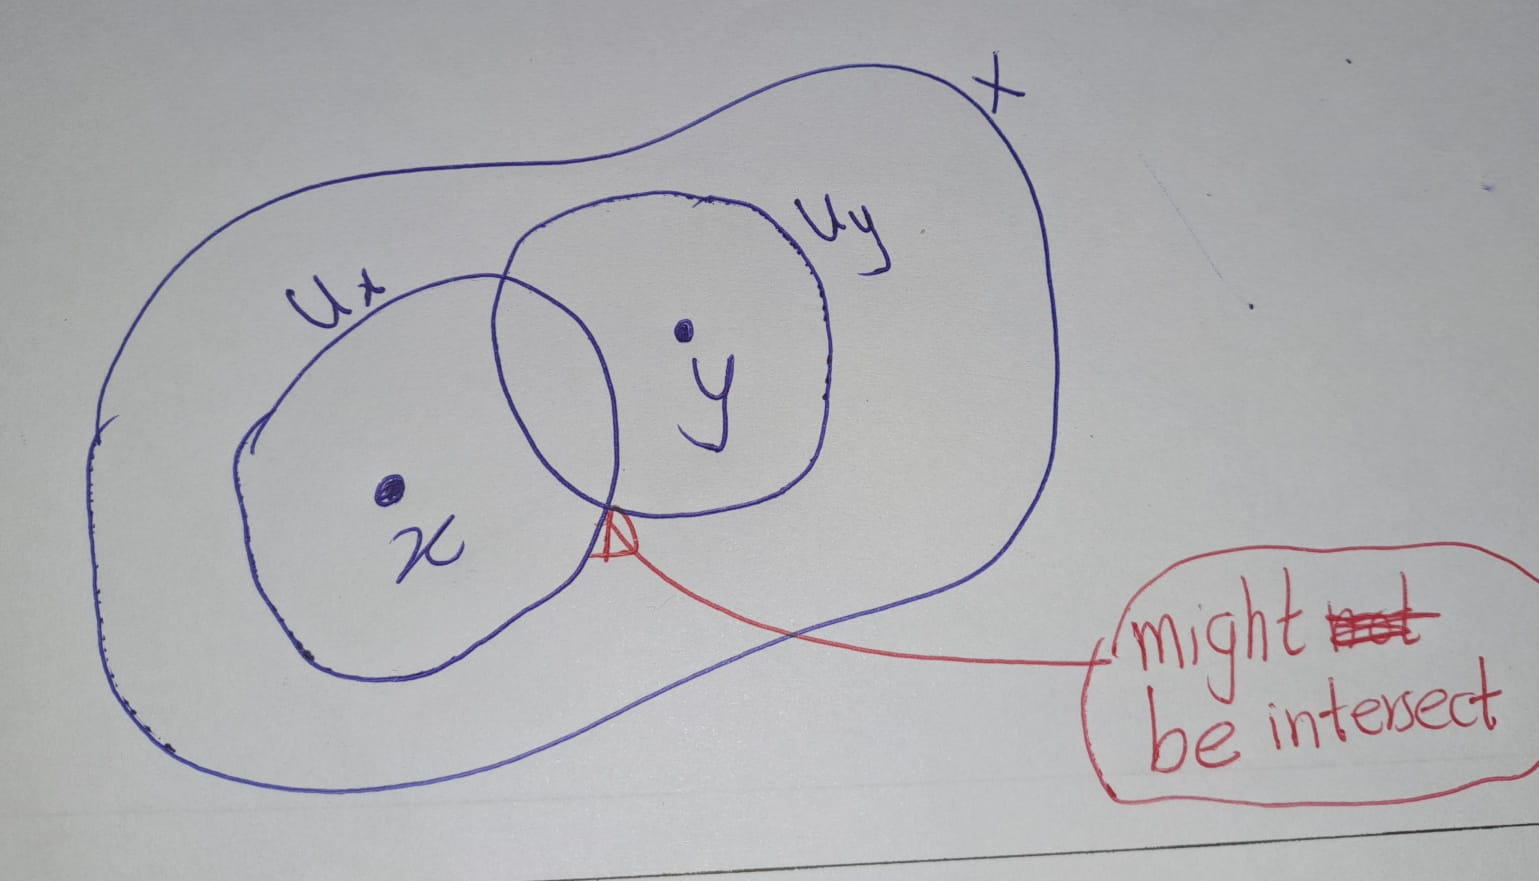
\includegraphics{figures/figure 17.jpg}
\caption{\label{fig:fig17}\(~\)}
\end{figure}

These \(T_1\) and \(T_2\) axioms are called the separation axioms.

\begin{example}
\protect\hypertarget{exm:unnamed-chunk-78}{}\label{exm:unnamed-chunk-78}Let \(X\) b a set. Consider \(X\) with finite complemenet topology is \(T_1\) Space. (i.e.:\((X,\mathcal{T}_f)\) is \(T_1\) space.) But \(X\) is not \(T_2\) if \(X\) is infinite.
\end{example}

\textbf{Claim 1} : \((X,\mathcal{T}_{f})\) is \(T_1\) space.

\begin{proof}

Let \(x,y\in X\). Then

\begin{itemize}
\tightlist
\item
  \(X\setminus \{x\}\) is an open set of \(\mathcal{T}_{f}\) containing \(y\) but not \(x\).
\item
  \(X\setminus \{y\}\) is an open set of \(\mathcal{T}_{f}\) containing \(x\)
  but not \(y\).
  Hence the result from definition of \(T_1\) space.
\end{itemize}

\end{proof}

\textbf{Claim 2} : \(X\) is not \(T_2\) if \(X\) is infinite.

\begin{proof}
Let \(x_1,x_2\in X\) with \(x_1\neq x_2\) Suppose \(x_1,x_2\) have disjoint neighbhood \(U_1\) and \(U_2\). I.e.: \(U_1\cap U_2=\emptyset\). Thus
\begin{eqnarray}
X &=& X\setminus (U_1\cap U_2)\\
&=& \underbrace{(X \setminus U_1 )}_{\text{finite}} \cup \underbrace{(X\setminus U_2)}_{\text{finite}}
\end{eqnarray}
Note that both \((X \setminus U_1 )\) and \((X \setminus U_2 )\) are finite. Thus, X is finite. Hence, if \(X\) is \(T_2\) then \(X\) is finite. (Contrapostive of given statement). Therefore, if \(X\) is infinite then \(X\) is not \(T_2\).
\end{proof}

\begin{theorem}
\protect\hypertarget{thm:unnamed-chunk-81}{}\label{thm:unnamed-chunk-81}Every finite point set in a Hausdorff space \(X\) is closed.
\end{theorem}

\begin{proof}
It suffices to show that every one-point set \(\{x_0\}\) is closed. If \(x\) is a point of \(X\)
different from \(x_0\), then \(x\) and \(x_0\) have disjoint neighborhoods \(U\) and \(V\), respectively.
Since \(U\) does not intersect \(\{x_0\}\), the point \(x\) cannot belong to the closure of the set \(\{x_0\}\).
As a result, the closure of the set \(\{x_0\}\) is \(\{x_0\}\) itself, so that it is closed.
\end{proof}

\begin{definition}
\protect\hypertarget{def:unnamed-chunk-83}{}\label{def:unnamed-chunk-83}Let \(X\) be topological sapce. A sequence \(x_1,x_2,x_3,...\) in \(X\) \textbf{converges} to \(x\in X\) if for every neighborhood \(U\) of \(x\) there exists \(N\in \mathbb{N}\) such that \(x_n \in U\) for all \(n\geq N\)

Notataion: \(x_n \to x\)
\end{definition}

\begin{figure}
\centering
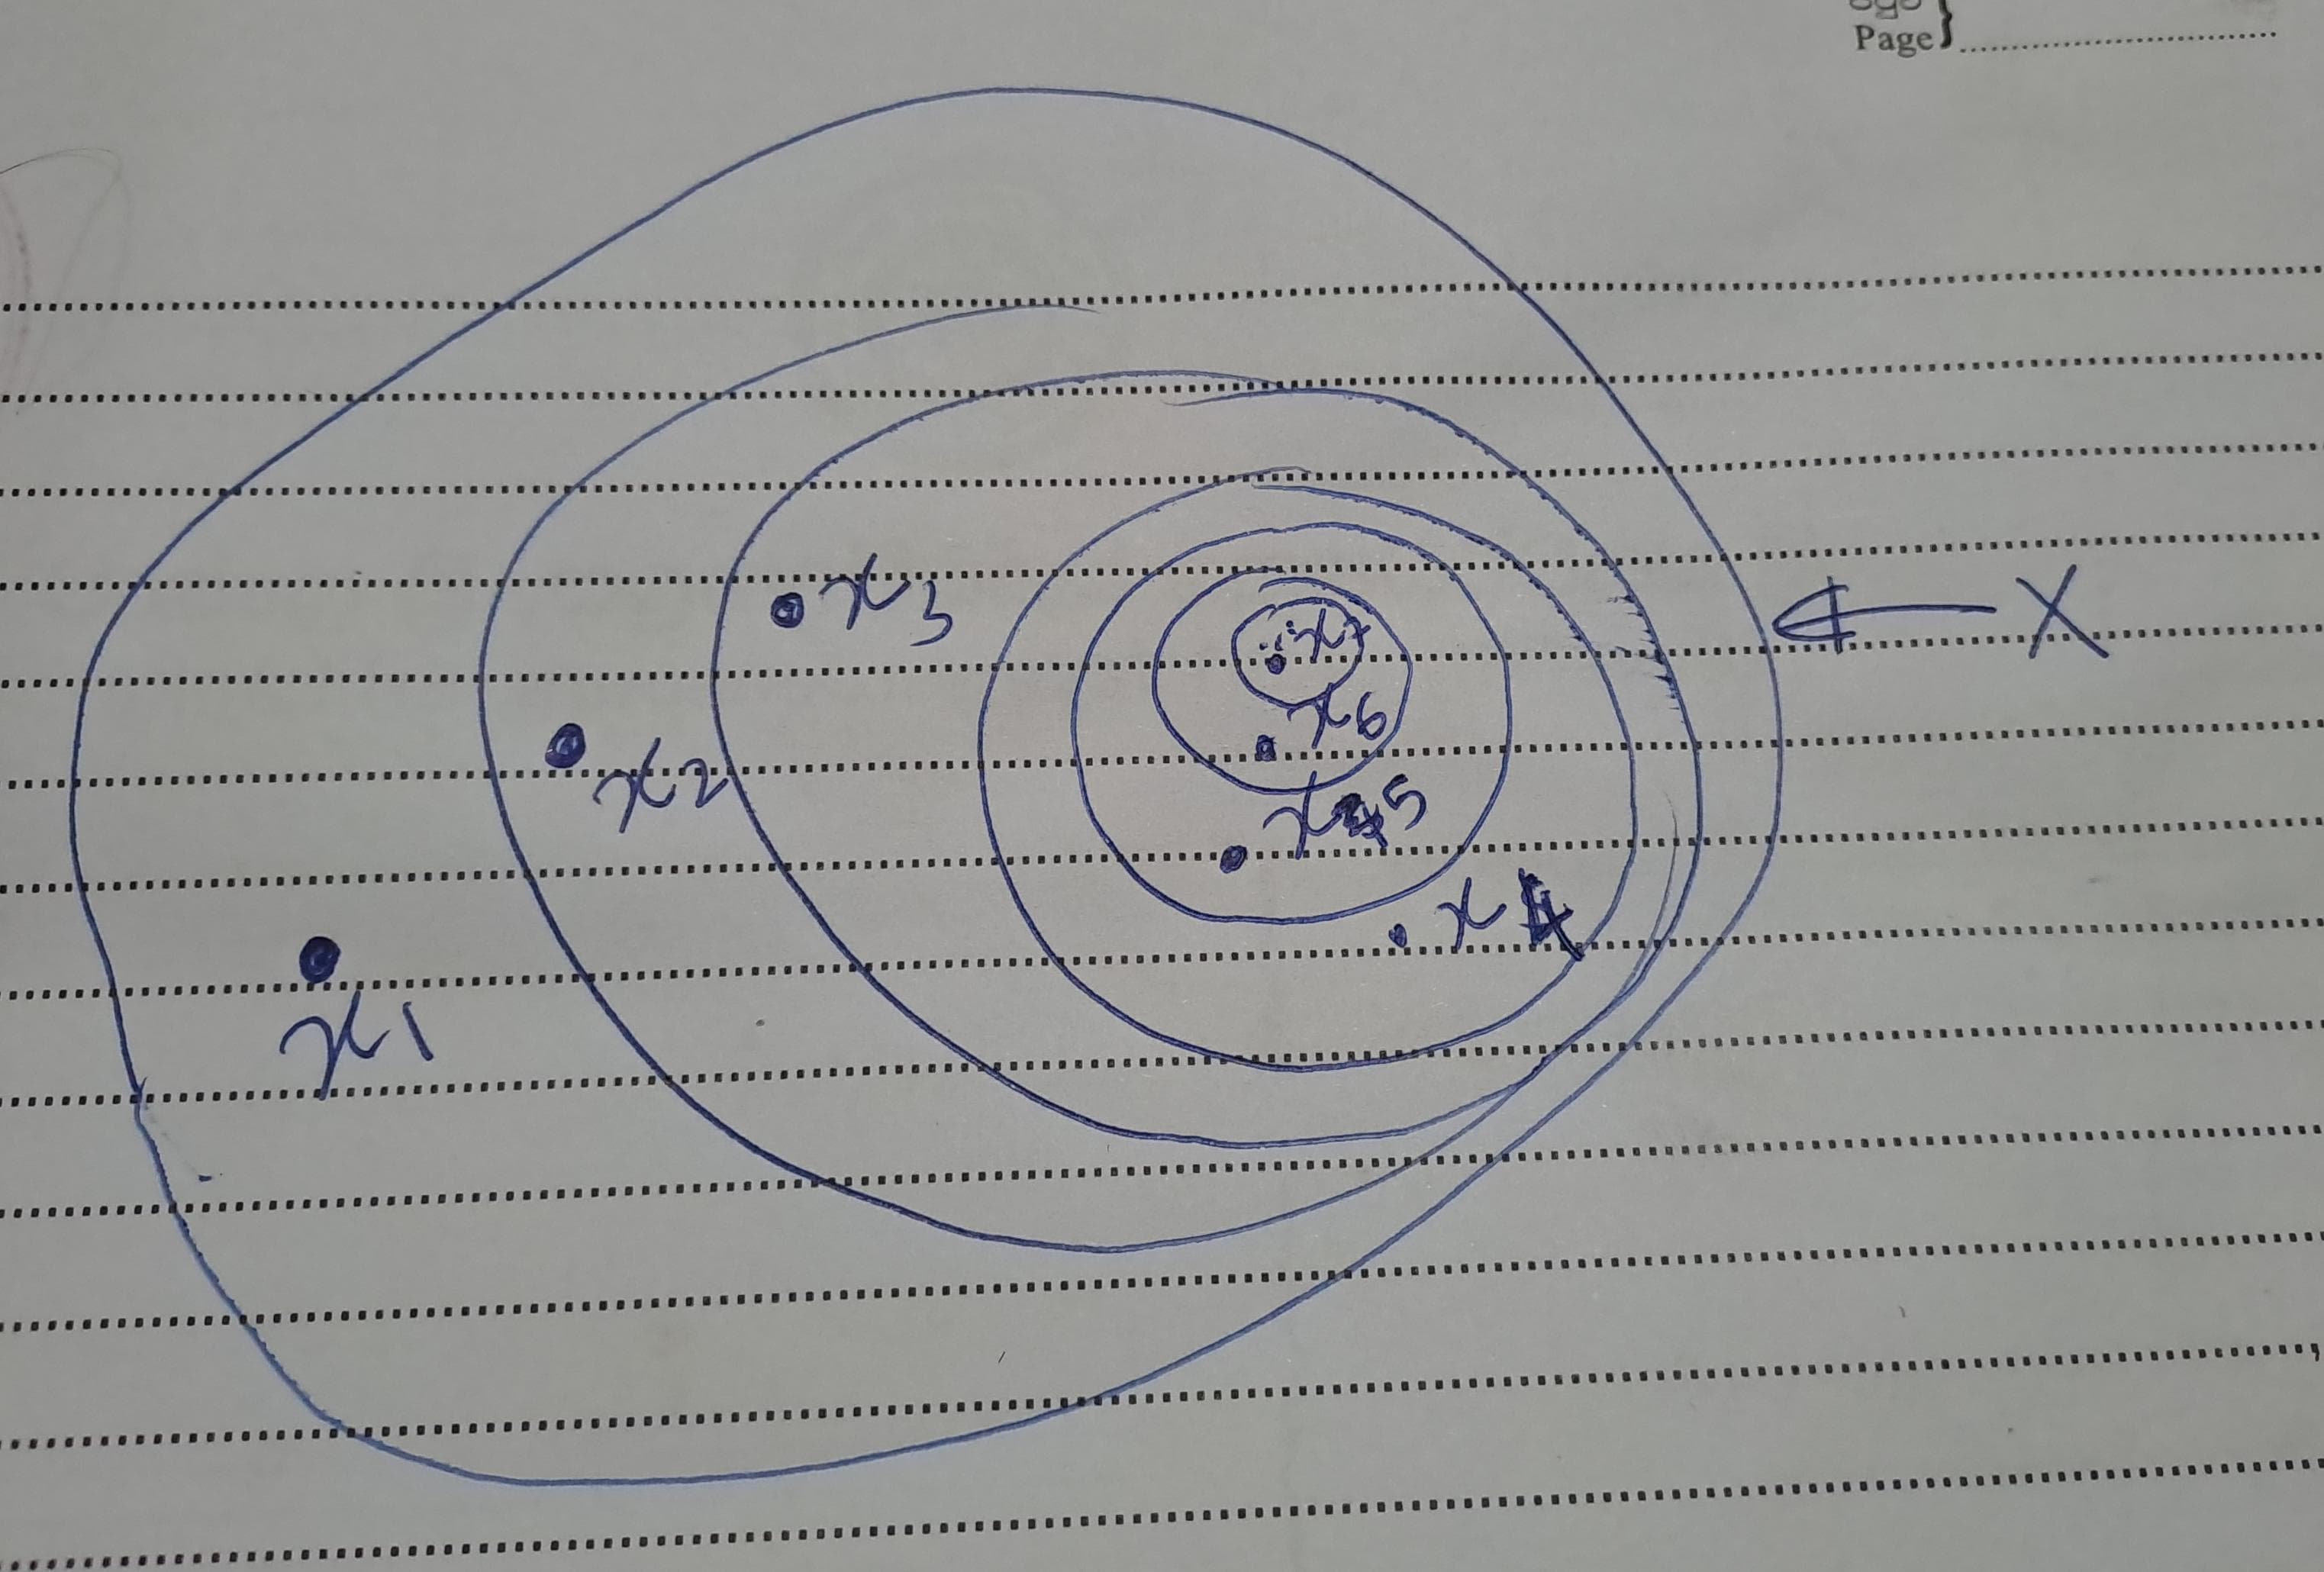
\includegraphics{figures/figure 18.jpg}
\caption{\label{fig:fig18}\(~\)}
\end{figure}

\begin{theorem}
\protect\hypertarget{thm:unnamed-chunk-84}{}\label{thm:unnamed-chunk-84}Let \(X\) be a Hausdorff space. If \(x_n\) convergence the limit \(x\) is unique.\\
In other words: The limit of a convergent sequence in a Hausdorff space is unique.
\end{theorem}

\begin{proof}
We are going to indirect proof. Assume that \(x_n \to x\) and \(x_n \to y\) and \(x\neq y\). Since \(X\) is a Hausdorff space, there are disjoint open sets \(U\) and \(V\) of \(X\) such that \(x\in U\) and \$ y\in V\$.

\begin{itemize}
\tightlist
\item
  Since \(x_n \to x\), \(U\) is an open neighbourhood of \(x\), there is a \(N_0\in \mathbb{N}\) , such that \(x_n \in U\) for all \(n\geq N_0\)
\item
  Since \(x_n \to y\), \(V\) is an open neighbourhood of \(y\), there is a \(N_1\in \mathbb{N}\) , such that \(x_n \in V\) for all \(n\geq N_1\)
\end{itemize}

Let \(N=max\{N_0,N_1\}\).
Since \(N>N_0\), then \(x_N\in U\).
Since \(N>N_1\), then \(x_N\in V\).
Thus, \(x_N\in U \cap V\). This contardict disjointness the \(u\) and \(V\). Thefore, \(x=y\)
\end{proof}

\begin{theorem}
\protect\hypertarget{thm:unnamed-chunk-86}{}\label{thm:unnamed-chunk-86}Let \(X\) be a Hausdorff space and \(A\subseteq X\). Then,\\
\(x\in X\) is a limit point \(\iff\) every neighbourhood intersect \(A\) is infinetly many points.
\end{theorem}

\begin{proof}
\leavevmode

\begin{itemize}
\item
  (\(\Longleftarrow\)) First suppose that every neighborhood of \(x\) intersects \(A\) in infinitely many points, it certainly intersects \(A\) in some point other than \(x\) itself, so that \(x\) is a limit point of \(A\).
\item
  (\(\Longrightarrow\)) Now suppose that \(x\) is a limit point of \(A\). We are going to use proof by contradiction. Assume that there is some neighborhood \(U\) of \(x\) intersects \(A\) in only finitely many points.
  Then \(U\) also intersects \(A - \{x\}\) in finitely many points. Let \(\{x_1,..., x_m\}\) be the points of \(U \cap (A - \{x\})\).
  i.e.: \[U \cap (A - \{x\})=\{x_1,..., x_m\}\]
  The set \(X - \{x_1,..., x_m\}\) is an open set of \(X\), since the finite point set \(\{x_1,..., x_m\}\) is closed. (By pervious theorem) Then \[U \cap (X - \{x_1,..., x_m\})\] is a neighborhood of \(x\) that intersects the set \(A - \{x\}\) not at all. This contradicts the assumption that \(x\) is a limit point of \(A\).
\end{itemize}

\end{proof}

\begin{theorem}
\protect\hypertarget{thm:unnamed-chunk-88}{}\label{thm:unnamed-chunk-88}If \(X\) is a Hausdorff space, then a sequence of points of \(X\) converges to at most one point of \(X\).
\end{theorem}

\begin{proof}
Suppose that \(x_n\) is a sequence of points of \(X\) that converges to \(x\). If \(y \neq x\), let \(U\) and \(V\) be disjoint neighbourhoods of \(x\) and \(y\), respectively. Since \(U\) contains \(x_n\) for all but finitely many values of \(n\). (It contain all terms with out some finetely many terms) Since \(U \cap V=\emptyset\), the set \(V\) cannot caontain those terms. Therefore, \(x_n\) cannot converge to \(y\).
\end{proof}

\begin{definition}[Limit of a sequence]
\protect\hypertarget{def:unnamed-chunk-90}{}\label{def:unnamed-chunk-90}If the sequence \(x_n\) of points of the Hausdorff space \(X\) converges to the point \(x\) of \(X\), we often write \(x_n \to x\), and we say that \(x\) is the \textbf{limit} of the sequence \(x_n\).
\end{definition}

\begin{theorem}
\protect\hypertarget{thm:unnamed-chunk-91}{}\label{thm:unnamed-chunk-91}\leavevmode

\begin{itemize}
\tightlist
\item
  Every simply ordered set is a Hausdorff space in the order topology.
\item
  The product of two Hausdorff spaces is a Hausdorff space.
\item
  A subspace of a Hausdorff space is a Hausdorff space.
\end{itemize}

\end{theorem}

\begin{proof}
See exercise \ref{exr:Hausdorff1},\ref{exr:Hausdorff2} and \ref{exr:Hausdorff3}
\end{proof}

\hypertarget{continuous-functions}{%
\section{Continuous Functions}\label{continuous-functions}}

\hypertarget{continuity-of-a-function}{%
\subsection{Continuity of a Function}\label{continuity-of-a-function}}

\begin{definition}
\protect\hypertarget{def:unnamed-chunk-93}{}\label{def:unnamed-chunk-93}Let \(X\) and \(Y\) be topological spaces. A function \(f : X \to Y\) is said to be continuous if for each open subset \(V\) of \(Y\) , the set \(f^{−1}(V)\) is an open subset of \(X\).
\end{definition}

Recall that,
\[f^{ −1}(V)=\{x\in X: f(x)\in V\}\]

\begin{remark}
\leavevmode

\begin{itemize}
\tightlist
\item
  If it is empty if \(V\) does not intersect the image set \(f (X)\) of \(f\) .
\item
  Continuity of a function depends \emph{not} only upon the function \(f\) itself, but also on the topologies specified for its domain and range.\\
  I like to emphasize this fact, we can say that \(f\) is continuous \emph{relative} to specific topologies on \(X\) and \(Y\).
\end{itemize}

\end{remark}

\hypertarget{chapter-2-name}{%
\chapter{Chapter 2 name}\label{chapter-2-name}}

\hypertarget{chapter-03-name}{%
\chapter{Chapter 03 name}\label{chapter-03-name}}

Up to there is none.

\hypertarget{post-after-verify}{%
\section{Post After verify}\label{post-after-verify}}

\begin{enumerate}
\def\labelenumi{\alph{enumi}.}
\item
  \textbf{Interior of a set is open in X:} The interior of a set \(S\), denoted by \(\text{int}(S)\), is defined as the union of all open sets contained in \(S\). Since the union of open sets is open, \(\text{int}(S)\) is open in \(X\).
\item
  \textbf{If \(T\) is open in \(X\) then \(T \subseteq S\) if and only if \(T \subseteq \text{int}(S)\):} If \(T\) is an open set and \(T \subseteq S\), then every point in \(T\) is an interior point of \(S\). Therefore, \(T \subseteq \text{int}(S)\). Conversely, if \(T \subseteq \text{int}(S)\), then \(T\) is a subset of \(S\).
\item
  \textbf{Interior of \(S\) is an open subset of \(S\) when \(S\) is given the subspace topology:} The interior of a set \(S\), \(\text{int}(S)\), is the union of all open sets contained in \(S\). Therefore, \(\text{int}(S)\) is an open subset of \(S\).
\item
  \textbf{\(S\) is an open subset of \(X\) if and only if \(\text{int}(S) = S\):} If \(S\) is open, then every point of \(S\) is an interior point of \(S\), so \(\text{int}(S) = S\). Conversely, if \(\text{int}(S) = S\), then \(S\) is open because the interior of a set is always open.
\item
  \textbf{Interior operator preserves/distributes over binary intersection:} The interior of the intersection of two sets \(S\) and \(T\), \(\text{int}(S \cap T)\), is equal to the intersection of the interiors of \(S\) and \(T\), \(\text{int}(S) \cap \text{int}(T)\). This is because the intersection of two open sets is open, and the interior of a set is the union of all open sets contained in it.
\item
  \textbf{The interior operator does not distribute over unions:} The interior of the union of two sets \(S\) and \(T\), \(\text{int}(S \cup T)\), is a superset of the union of the interiors of \(S\) and \(T\), \(\text{int}(S) \cup \text{int}(T)\). This is because the union of two open sets is open, and the interior of a set is the union of all open sets contained in it. However, the equality might not hold in general. For example, if \(X = \mathbb{R}\), \(S = (-\infty, 0]\), and \(T = (0, \infty)\), then \(\text{int}(S) \cup \text{int}(T) = (-\infty, 0) \cup (0, \infty) = \mathbb{R} \setminus \{0\}\), which is a proper subset of \(\text{int}(S \cup T) = \text{int}(\mathbb{R}) = \mathbb{R}\).
\end{enumerate}

\hypertarget{exercises}{%
\chapter{Exercises}\label{exercises}}

\hypertarget{section-13-in-munkrees-book}{%
\section{Section 13 in Munkrees book}\label{section-13-in-munkrees-book}}

\begin{exercise}[Mun 2.13.1]
\protect\hypertarget{exr:unnamed-chunk-95}{}\label{exr:unnamed-chunk-95}Let \(X\) be a topological space; let \(A\) be a subset of \(X\). Suppose that for each \(x \in A\) there is an open set \(U\) containing \(x\) such that \(U \subset A\). Show that \(A\) is open in \(X\).
\end{exercise}

\begin{proof}
Let \(X\) be a topological space. Let \(A\) be a subset of \(X\). Suppose that for each \(x \in A\). Then \(U_x\) be the open set that,
\[x\in U_x\subseteq A\]
Now consider,
\[U:=\bigcup_{x\in A}U_x.\]
Note that \(U\) is open. By defintion of toplogy.
Furthur, \(A=U\). Hence, \(A\) is open set.
\end{proof}

\begin{exercise}[Mun 2.13.3]
\protect\hypertarget{exr:unnamed-chunk-97}{}\label{exr:unnamed-chunk-97}Consider the nine topologies on the set X = \{a, b, c\} indicated in Example 1 of §12. Compare them; that is, for each pair of topologies, determine whether they are comparable, and if so, which is the finer.
\end{exercise}

\begin{figure}
\centering
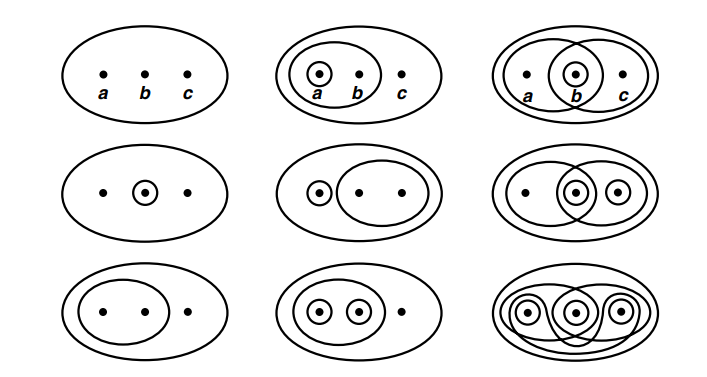
\includegraphics{figures/figure 01.png}
\caption{\label{fig:fig1}\(~\)}
\end{figure}

These topologies can be listed as follows,
\begin{align*}
\mathcal{T}_1 &= \{\emptyset, X\}, \\
\mathcal{T}_2 &= \{\emptyset, \{a\}, \{a, b\}, X\}, \\
\mathcal{T}_3 &= \{\emptyset, \{b\}, \{a, b\}, \{b, c\}, X\}, \\
\mathcal{T}_4 &= \{\emptyset, \{b\}, X\}, \\
\mathcal{T}_5 &= \{\emptyset, \{a\}, \{b, c\}, X\}, \\
\mathcal{T}_6 &= \{\emptyset, \{b\}, \{c\}, \{a, b\}, \{b, c\}, X\}, \\
\mathcal{T}_7 &= \{\emptyset, \{a, b\}, X\}, \\
\mathcal{T}_8 &= \{\emptyset, \{a\}, \{b\}, \{a, b\}, X\}, \\
\mathcal{T}_9 &= \{\emptyset, \{a\}, \{b\}, \{c\}, \{a, b\}, \{a, c\}, \{b, c\}, X\}.
\end{align*}
We can get following observations.
- \(\mathcal{T}_1\) is coarser than any other topology,
- \(\mathcal{T}_9\) is finer than any other topology.
- \(\mathcal{T}_7 \subset \mathcal{T}_2 \subset \mathcal{T}_8\)
- \(\mathcal{T}_4 \subset \mathcal{T}_3 \subset \mathcal{T}_6\)
- \(\mathcal{T}_7 \subset \mathcal{T}_3 \subset \mathcal{T}_6\)
- \(\mathcal{T}_4 \subset \mathcal{T}_8\).

\begin{exercise}
\protect\hypertarget{exr:unnamed-chunk-98}{}\label{exr:unnamed-chunk-98}Show that the collection \(\mathcal{T}_c\) given in Example 4 of §12 (in Munkrees book) is a topology on the set \(X\).
Is the collection
\[\mathcal{T}_{\infty} = \{U | X - U \text{ is infinite or empty or all of } X\}\]
a topology on \(X\)?
\end{exercise}

\begin{proof}

(Proof of \(\mathcal{T}_c\) is toplogy.)
Recall: \(\mathcal{T}_c\) is the collection of all subsets \(U\) of \(X\) such that \(X \setminus U\) is either countable or is all of \(X\).

\begin{itemize}
\item
  \(\emptyset\in \mathcal{T}_c\). (Beacuse \(X\setminus \emptyset=X\))\\
  \(X \in \mathcal{T}_c\). (Beacuse \(X\setminus X=\emptyset\) is countable)\\
  So, \(\emptyset\) and \(X\) are both in \(\mathcal{T}_c\).
\item
  Let \(\{U_\alpha\}_{\alpha \in J}\) be a family of sets in \(\mathcal{T}_c\). Then
  \[X \setminus \bigcup_{\alpha \in J} U_\alpha = \bigcap_{\alpha \in J} (X \setminus U_\alpha)\quad\text{ (By De Moragons Law)}\]
  is an intersection of countable sets, hence countable.
\item
  If \(U_1, \ldots, U_n\) are elements in \(\mathcal{T}_c\), then
  \[X \setminus \bigcap_{i=1}^{n} U_i = \bigcup_{i=1}^{n} (X \setminus U_i)quad\text{ (By De Moragons Law)}\]
  is countable being a union of countable sets. It follows that \(\mathcal{T}_c\) is a topology on \(X\).
\end{itemize}

\end{proof}

Note that \(\mathcal{T}_\infty\) is in general not a topology on \(X\).

\begin{itemize}
\tightlist
\item
  For example, let \(X = \mathbb{R}\),\\
  \(U_1 = (-\infty, 0)\) and \(U_2 = (0, \infty)\).\\
  Then \(U_1\) and \(U_2\) are in \(\mathcal{T}_\infty\) but \(U_1 \cup U_2 = \mathbb{R} \setminus \{0\}\) is not.
\end{itemize}

\begin{exercise}[Mun 2.13.4]
\protect\hypertarget{exr:unnamed-chunk-100}{}\label{exr:unnamed-chunk-100}\leavevmode

\begin{enumerate}
\def\labelenumi{(\alph{enumi})}
\tightlist
\item
  If \(\{\mathcal{T}_\alpha\}\) is a family of topologies on \(X\), show that \(\bigcap \mathcal{T}_\alpha\) is a topology on \(X\). Is \(\bigcup \mathcal{T}_\alpha\) a topology on \(X\)?
\item
  Let \(\{\mathcal{T}_\alpha\}\) be a family of topologies on \(X\). Show that there is a unique smallest topology on \(X\) containing all the collections \(\mathcal{T}_\alpha\), and a unique largest topology contained in all \(\mathcal{T}_\alpha\).
\item
  If \(X = \{a, b, c\}\), let
  \begin{align*}
  \mathcal{T}_1 &= \{\emptyset, X,\{a\},\{a, b\}\} \text{ and } \\
  \mathcal{T}_2 &= \{\emptyset, X,\{a\},\{b, c\}\}.
  \end{align*}
  Find the smallest topology containing \(\mathcal{T}_1\) and \(\mathcal{T}_2\), and the largest topology contained in \(\mathcal{T}_1\) and \(\mathcal{T}_2\).
\end{enumerate}

\end{exercise}

\textbf{Solution}:

\begin{enumerate}
\def\labelenumi{\alph{enumi})}
\tightlist
\item
\end{enumerate}

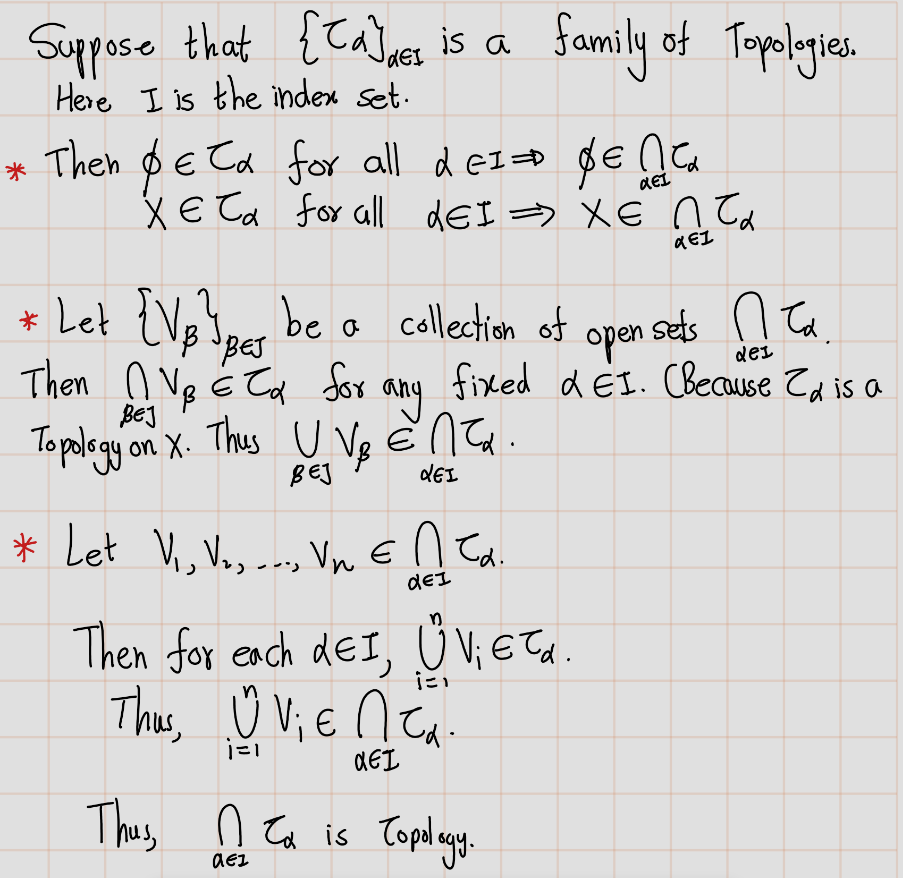
\includegraphics{figures/Exercises/Ex 2.13/ex-4-1.png}

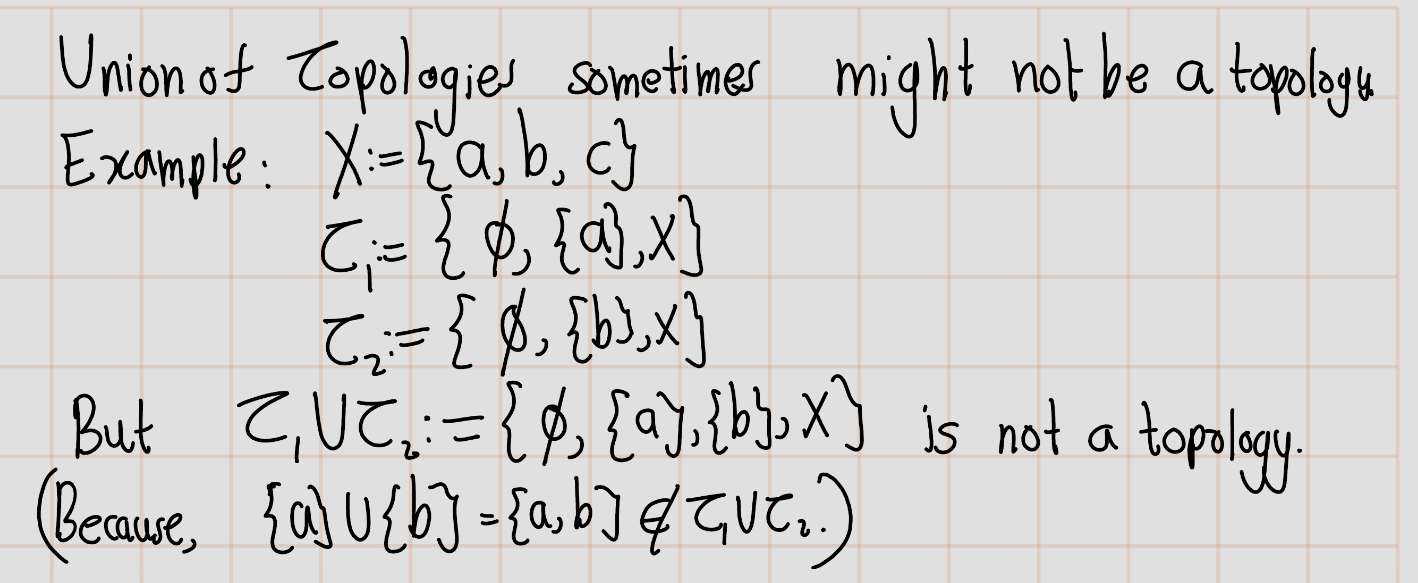
\includegraphics{figures/Exercises/Ex 2.13/ex-4-2.png}

\begin{enumerate}
\def\labelenumi{\alph{enumi})}
\setcounter{enumi}{1}
\tightlist
\item
\end{enumerate}

Let Let \(\{\mathcal{T}_\alpha\}\) be a family of topologies on \(X\).
Let \(\mathcal{F}:\{\mathcal{T}_\beta: \mathcal{T}_\beta\supseteq \bigcup \mathcal{T}_\alpha\}\) be family of topology that contain \(\bigcup\mathcal{T}_\alpha\).


\includegraphics{figures/Exercises/Ex 2.17/Notsure.png}
c)


\includegraphics{figures/Exercises/Ex 2.17/Notsure.png}

\begin{exercise}[Mun 2.13.5]
\protect\hypertarget{exr:unnamed-chunk-105}{}\label{exr:unnamed-chunk-105}Show that if \(A\) is a basis for a topology on \(X\), then the topology generated by \(A\) equals the intersection of all topologies on \(X\) that contain \(A\). Prove the same if \(A\) is a subbasis.
\end{exercise}

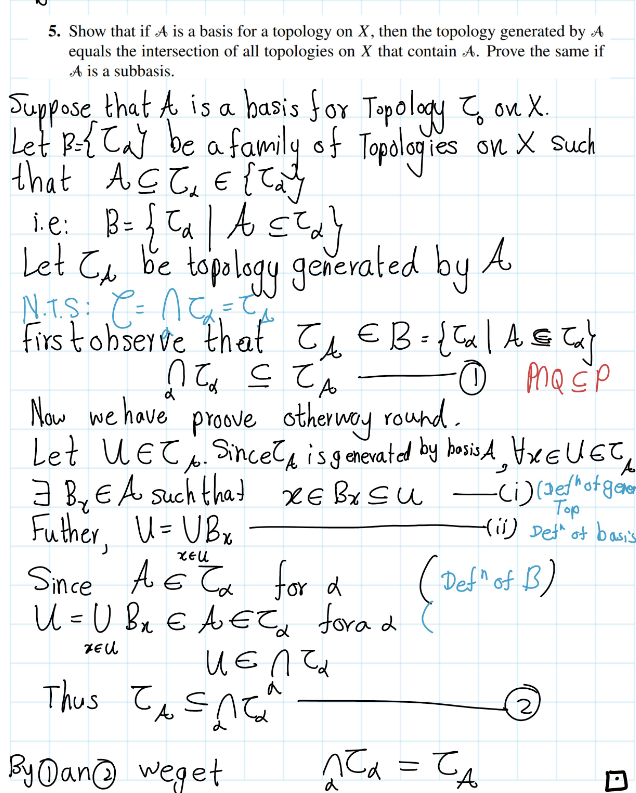
\includegraphics{figures/Exercises/Ex 2.13/ex-5-1.png}
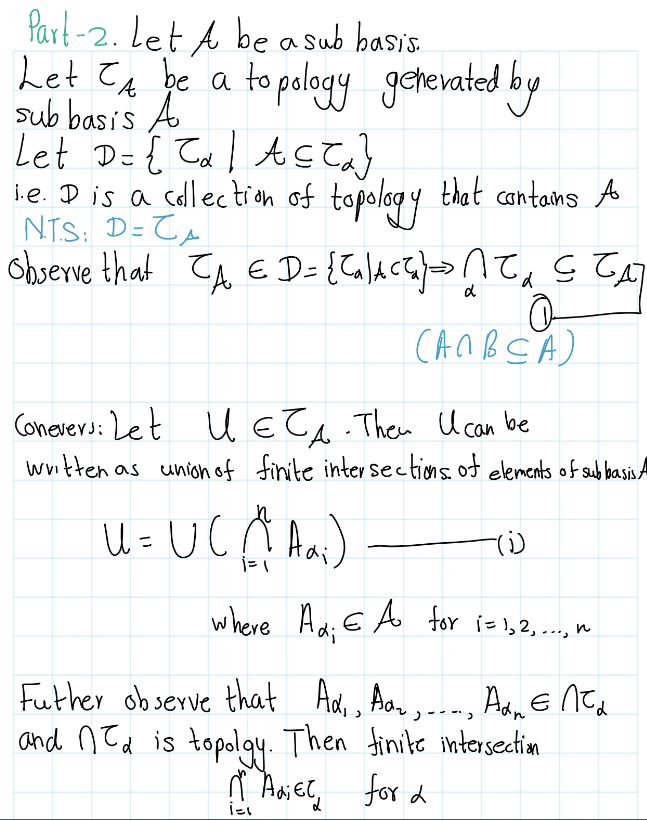
\includegraphics{figures/Exercises/Ex 2.13/ex-5-2.png}
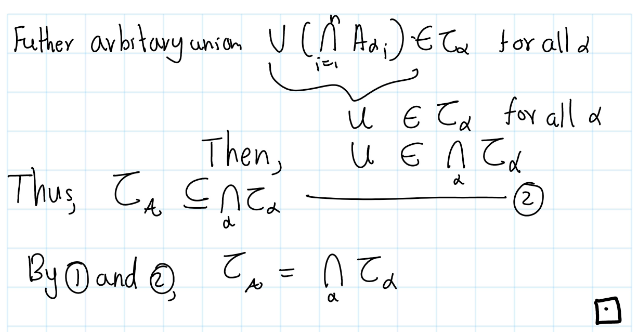
\includegraphics{figures/Exercises/Ex 2.13/ex-5-3.png}

\begin{exercise}[Mun 2.13.6]
\protect\hypertarget{exr:unnamed-chunk-109}{}\label{exr:unnamed-chunk-109}Show that the topologies of \(\mathbb{R}_l\) and \(\mathbb{R}_K\) are not comparable.
\end{exercise}

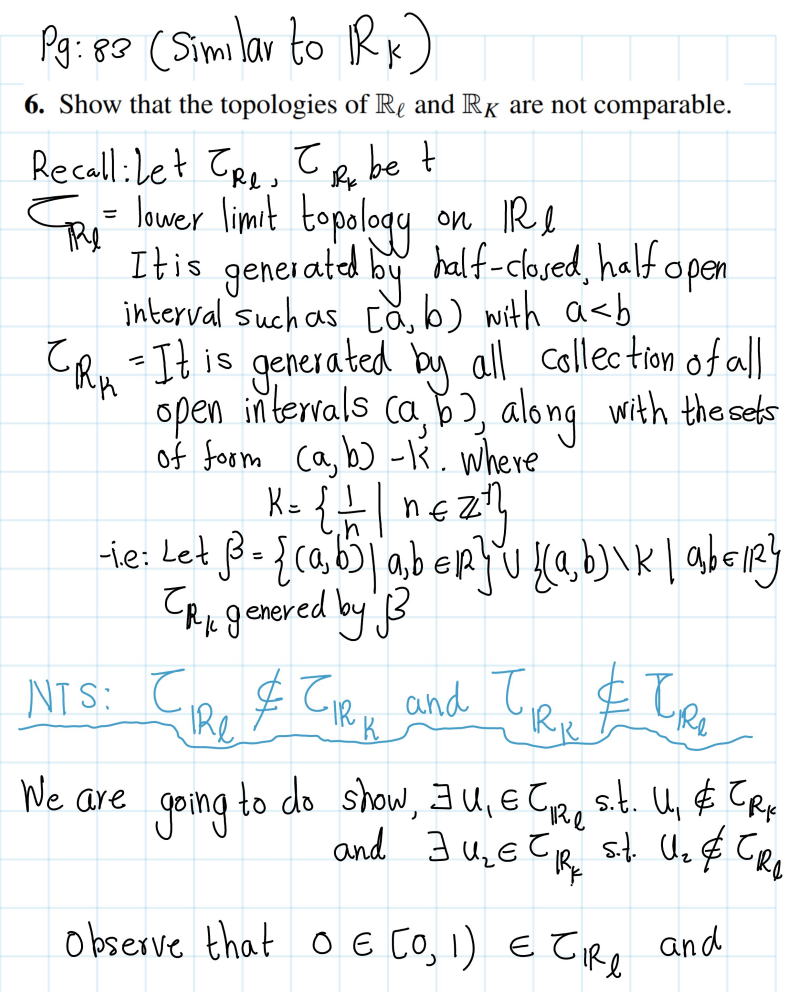
\includegraphics{figures/Exercises/Ex 2.13/ex-6-1.png}
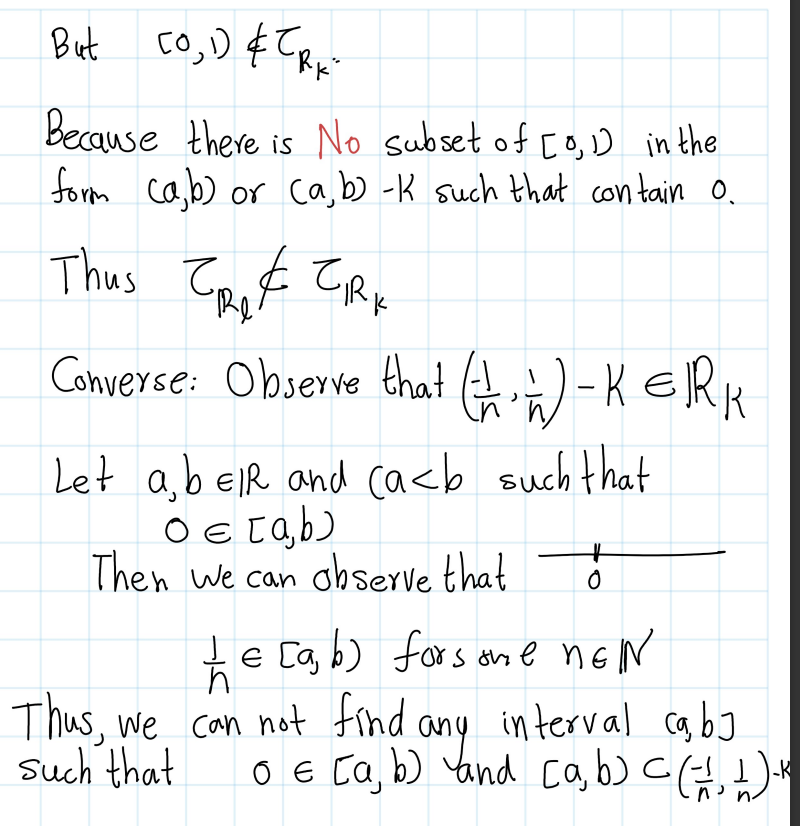
\includegraphics{figures/Exercises/Ex 2.13/ex-6-2.png}

\begin{exercise}
\protect\hypertarget{exr:unnamed-chunk-112}{}\label{exr:unnamed-chunk-112}Consider \(s\)
\end{exercise}

\hypertarget{section-16-in-munkress-book}{%
\section{Section 16 in Munkress Book}\label{section-16-in-munkress-book}}

\begin{exercise}[Mun 2.16.2]
\protect\hypertarget{exr:unnamed-chunk-113}{}\label{exr:unnamed-chunk-113}Show that if \(Y\) is a subspace of \$X, and \(A\) is a subset of \(Y\) , then the topology \(A\) inherits as a subspace of \(Y\) is the same as the topology it inherits as a subspace of \(X\).
\end{exercise}

\textbf{Solution}:
Let's denote the topology on \(X\) as \(\mathcal{T}_X\), the topology on \(Y\) as \(\mathcal{T}_Y\), and the topology on \(A\) as \(\mathcal{T}_A\).

We know that \(Y\) is a subspace of \(X\), so the topology \(\mathcal{T}_Y\) that \(Y\) inherits from \(X\) is \(\mathcal{T}_Y = \{ Y \cap U : U \in \mathcal{T}_X \}\).

Similarly, \(A\) is a subset of \(Y\), so the topology \(\mathcal{T}_A\) that \(A\) inherits from \(Y\) is \(\mathcal{T}_A = \{ A \cap V : V \in \mathcal{T}_Y \}\).

Substituting \(\mathcal{T}_Y\) into the equation for \(\mathcal{T}_A\), we get \(\mathcal{T}_A = \{ A \cap (Y \cap U) : U \in \mathcal{T}_X \}\).

Since \(A\) is a subset of \(Y\), \(A \cap Y = A\). So, \(\mathcal{T}_A = \{ A \cap U : U \in \mathcal{T}_X \}\).

This is exactly the topology that \(A\) would inherit as a subspace of \(X\). Therefore, the topology \(A\) inherits as a subspace of \(Y\) is the same as the topology it inherits as a subspace of \(X\).

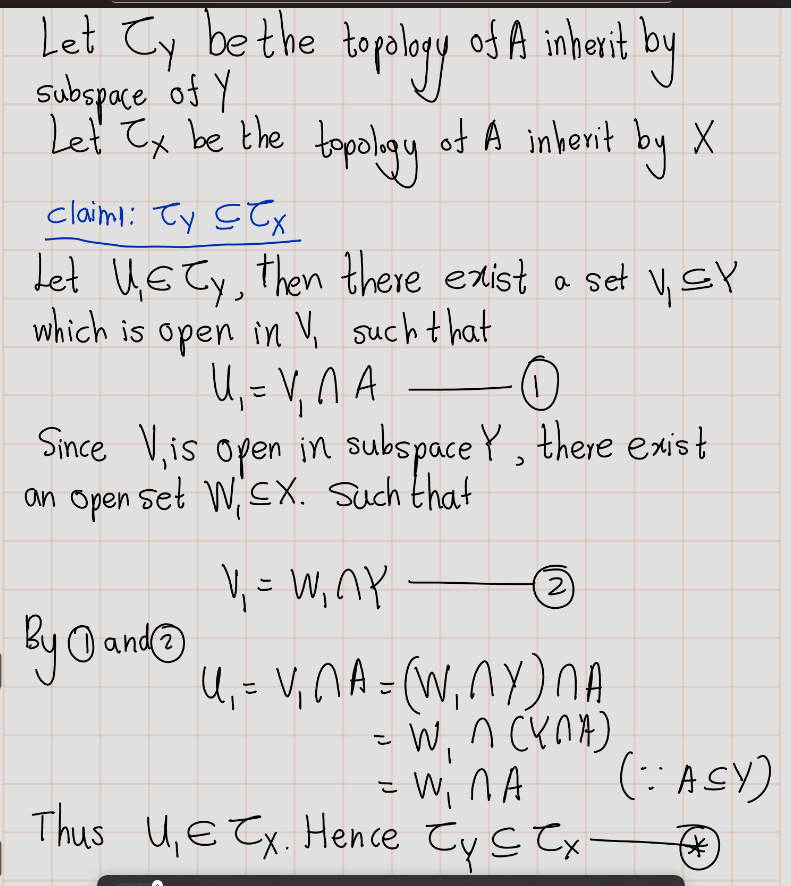
\includegraphics{figures/Exercises/Ex 2.16/ex1-1.png}

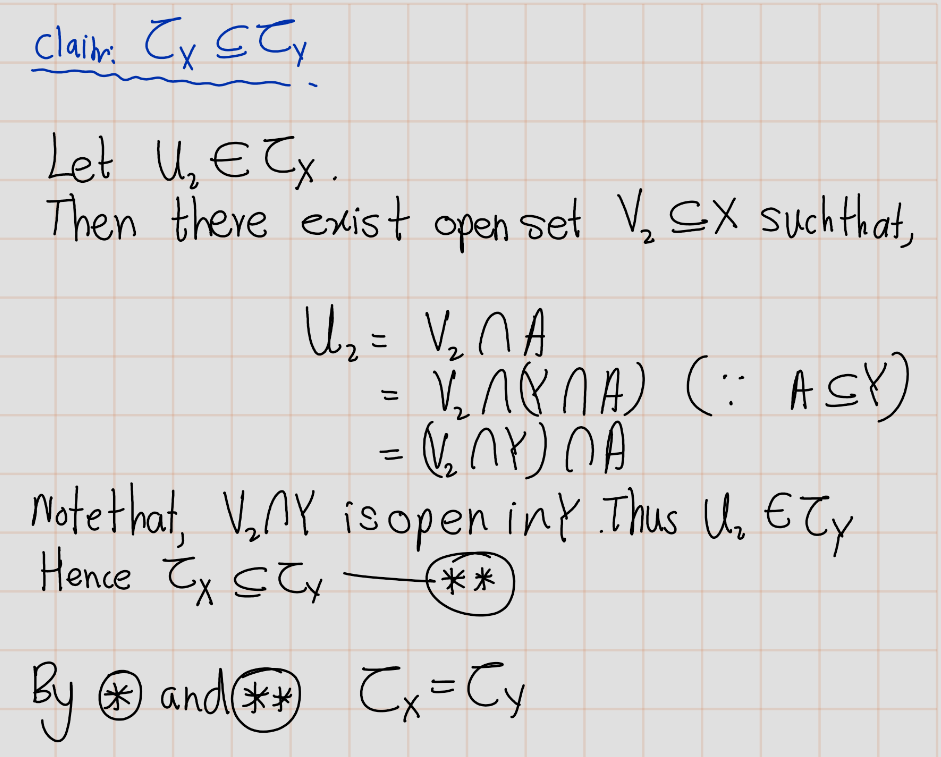
\includegraphics{figures/Exercises/Ex 2.16/ex1-2.png}

\begin{exercise}[Mun 2.16.2]
\protect\hypertarget{exr:unnamed-chunk-116}{}\label{exr:unnamed-chunk-116}If \(\mathcal{T}\) and \(\mathcal{T}\) are topologies on \(X\) and \(\mathcal{T}\) is strictly finer than \(\mathcal{T}\) , what can you
say about the corresponding subspace topologies on the subset \(Y\) of \(X\)?
\end{exercise}

\textbf{Solution}:
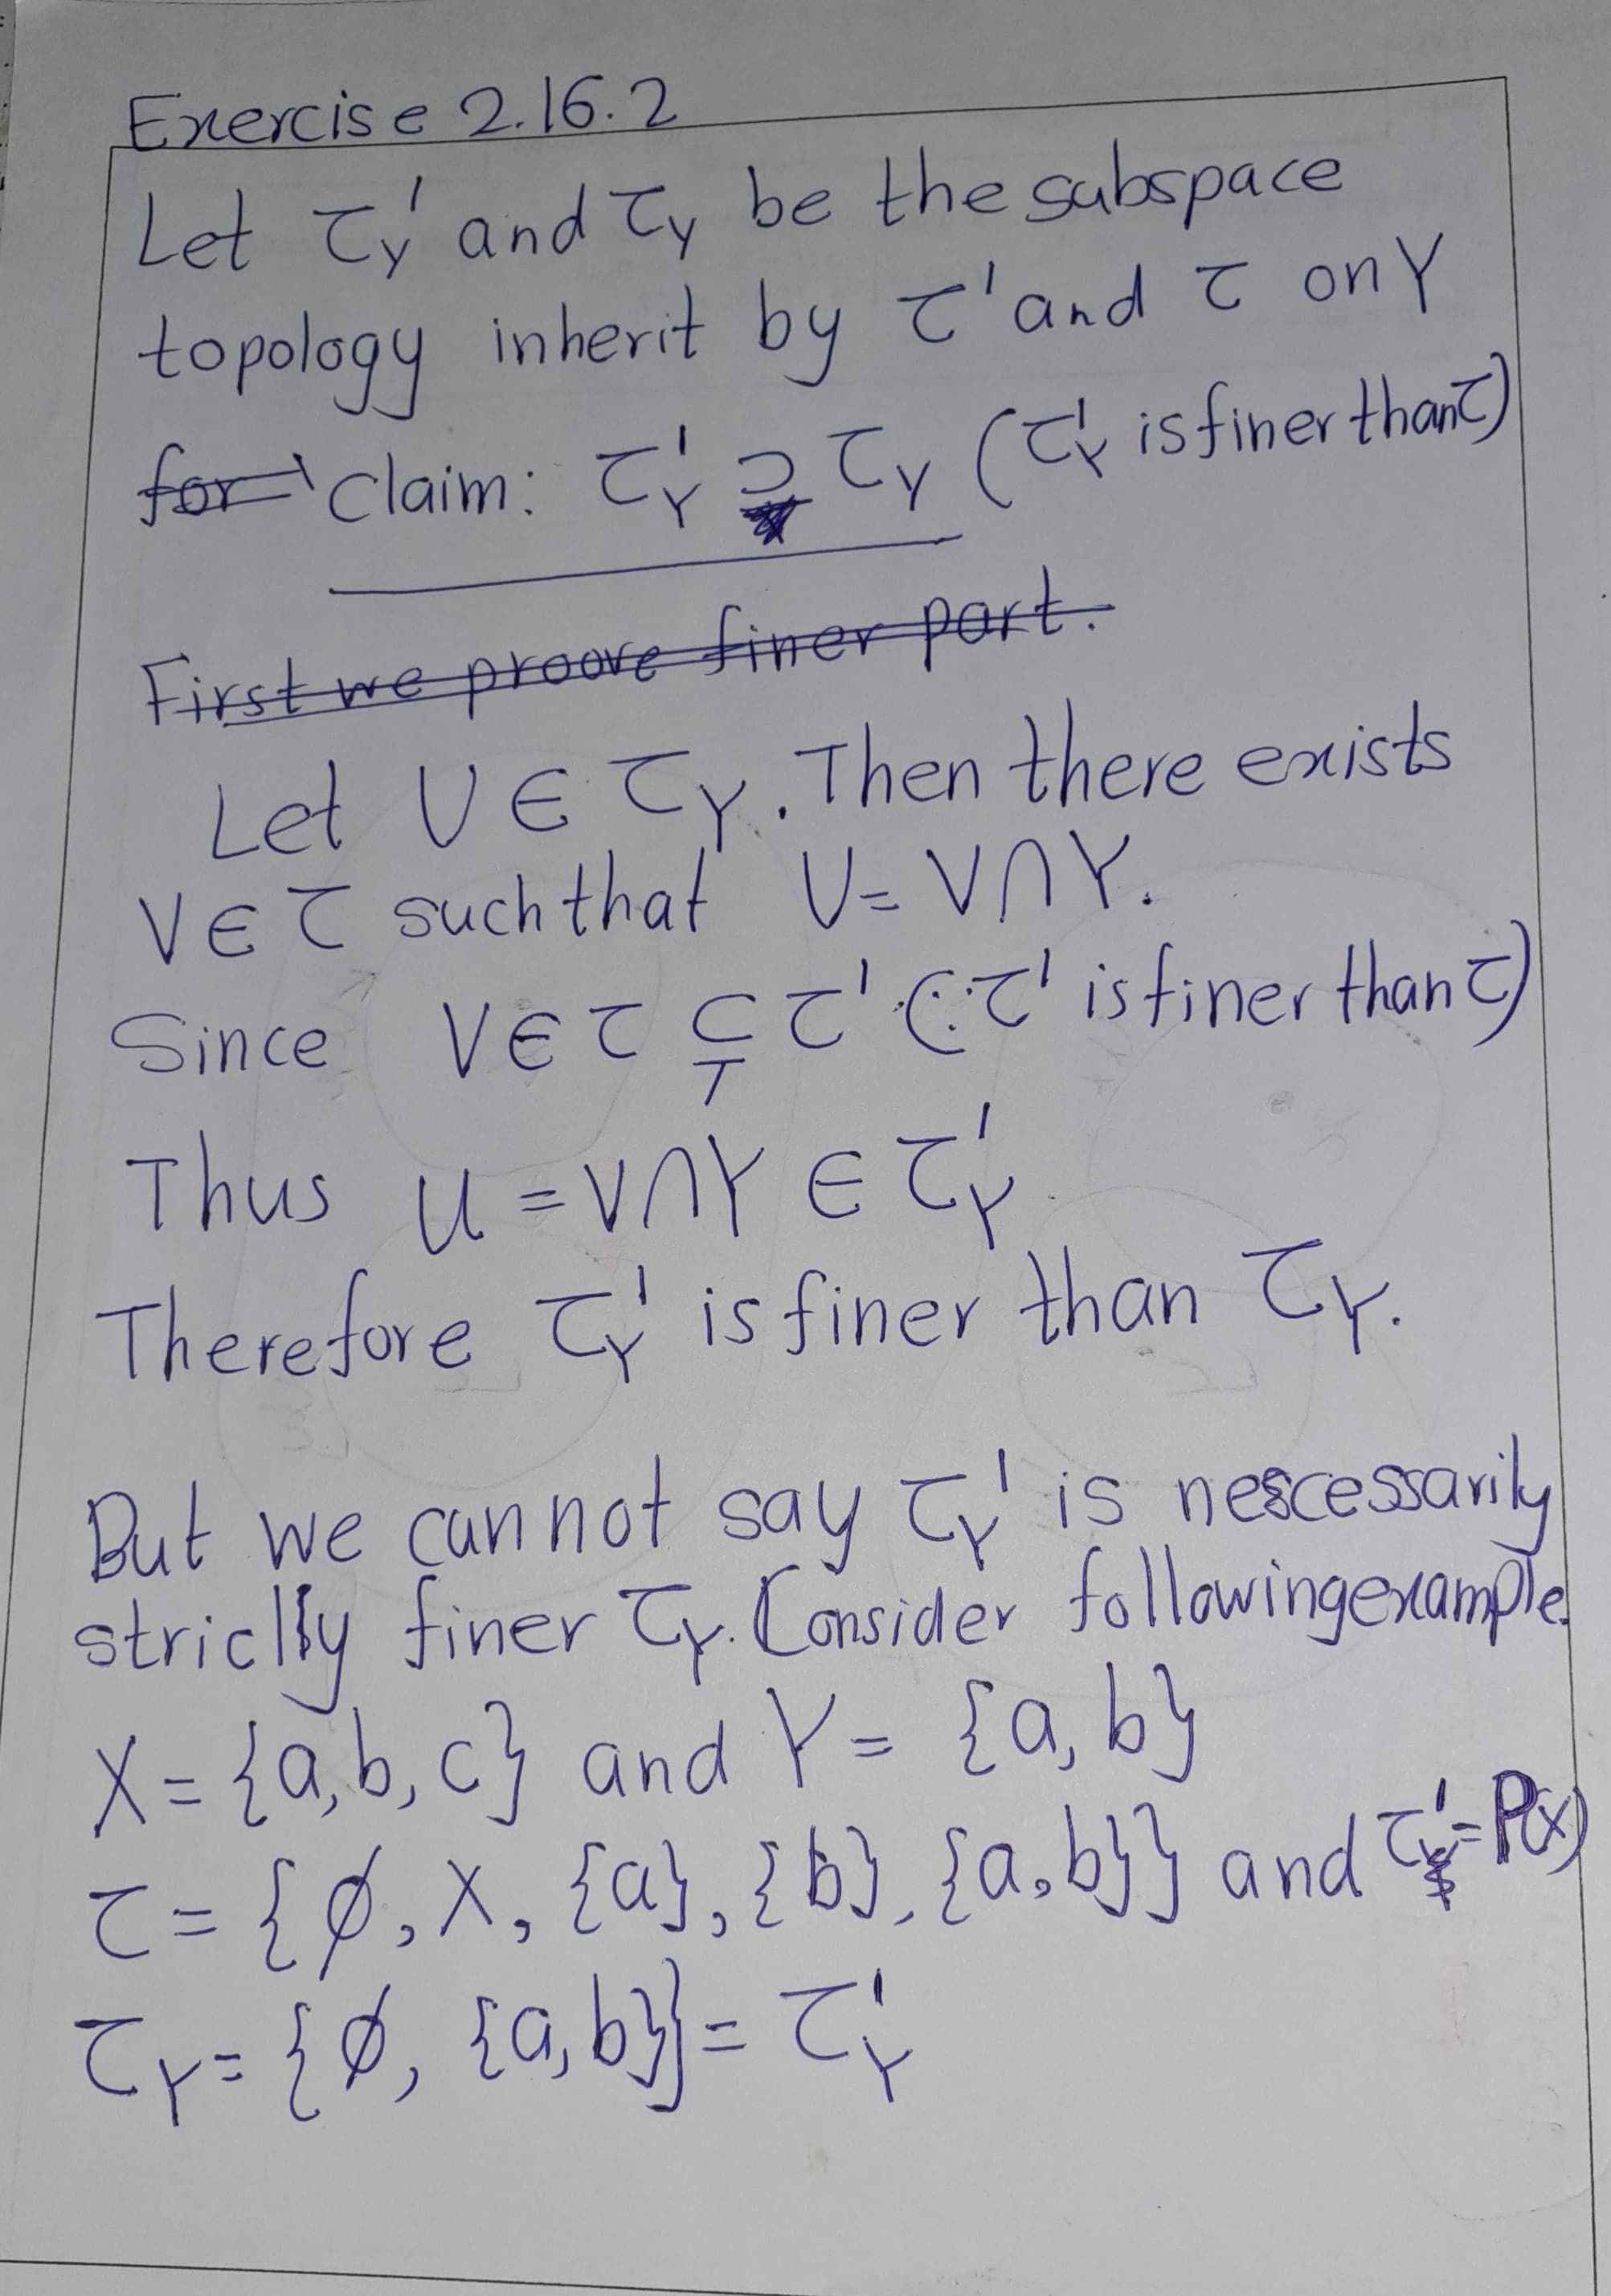
\includegraphics{figures/Exercises/Ex 2.16/ex-2.jpg}

\begin{exercise}[Mun 2.16.3]
\protect\hypertarget{exr:unnamed-chunk-118}{}\label{exr:unnamed-chunk-118}Consider the set \(Y = [−1, 1]\) as a subspace of \(\mathbb{R}\). Which of the following sets are open in \(Y\) ? Which are open in \(\mathbb{R}\)?
\begin{align}
A &= \{ x \mid \frac{1}{2} < |x| < 1 \}\\ 
B &= \{ x \mid \frac{1}{2} < |x| \leq 1 \} \\
C &= \{ x \mid \frac{1}{2} \leq |x| < 1 \}\\
D &= \{ x \mid \frac{1}{2} \leq |x| \leq 1 \}\\
E &= \{ x \mid 0 < |x| < 1 \text{ and } \frac{1}{x} \notin \mathbb{Z}^+ \}
\end{align}
\end{exercise}

\textbf{Solution}:
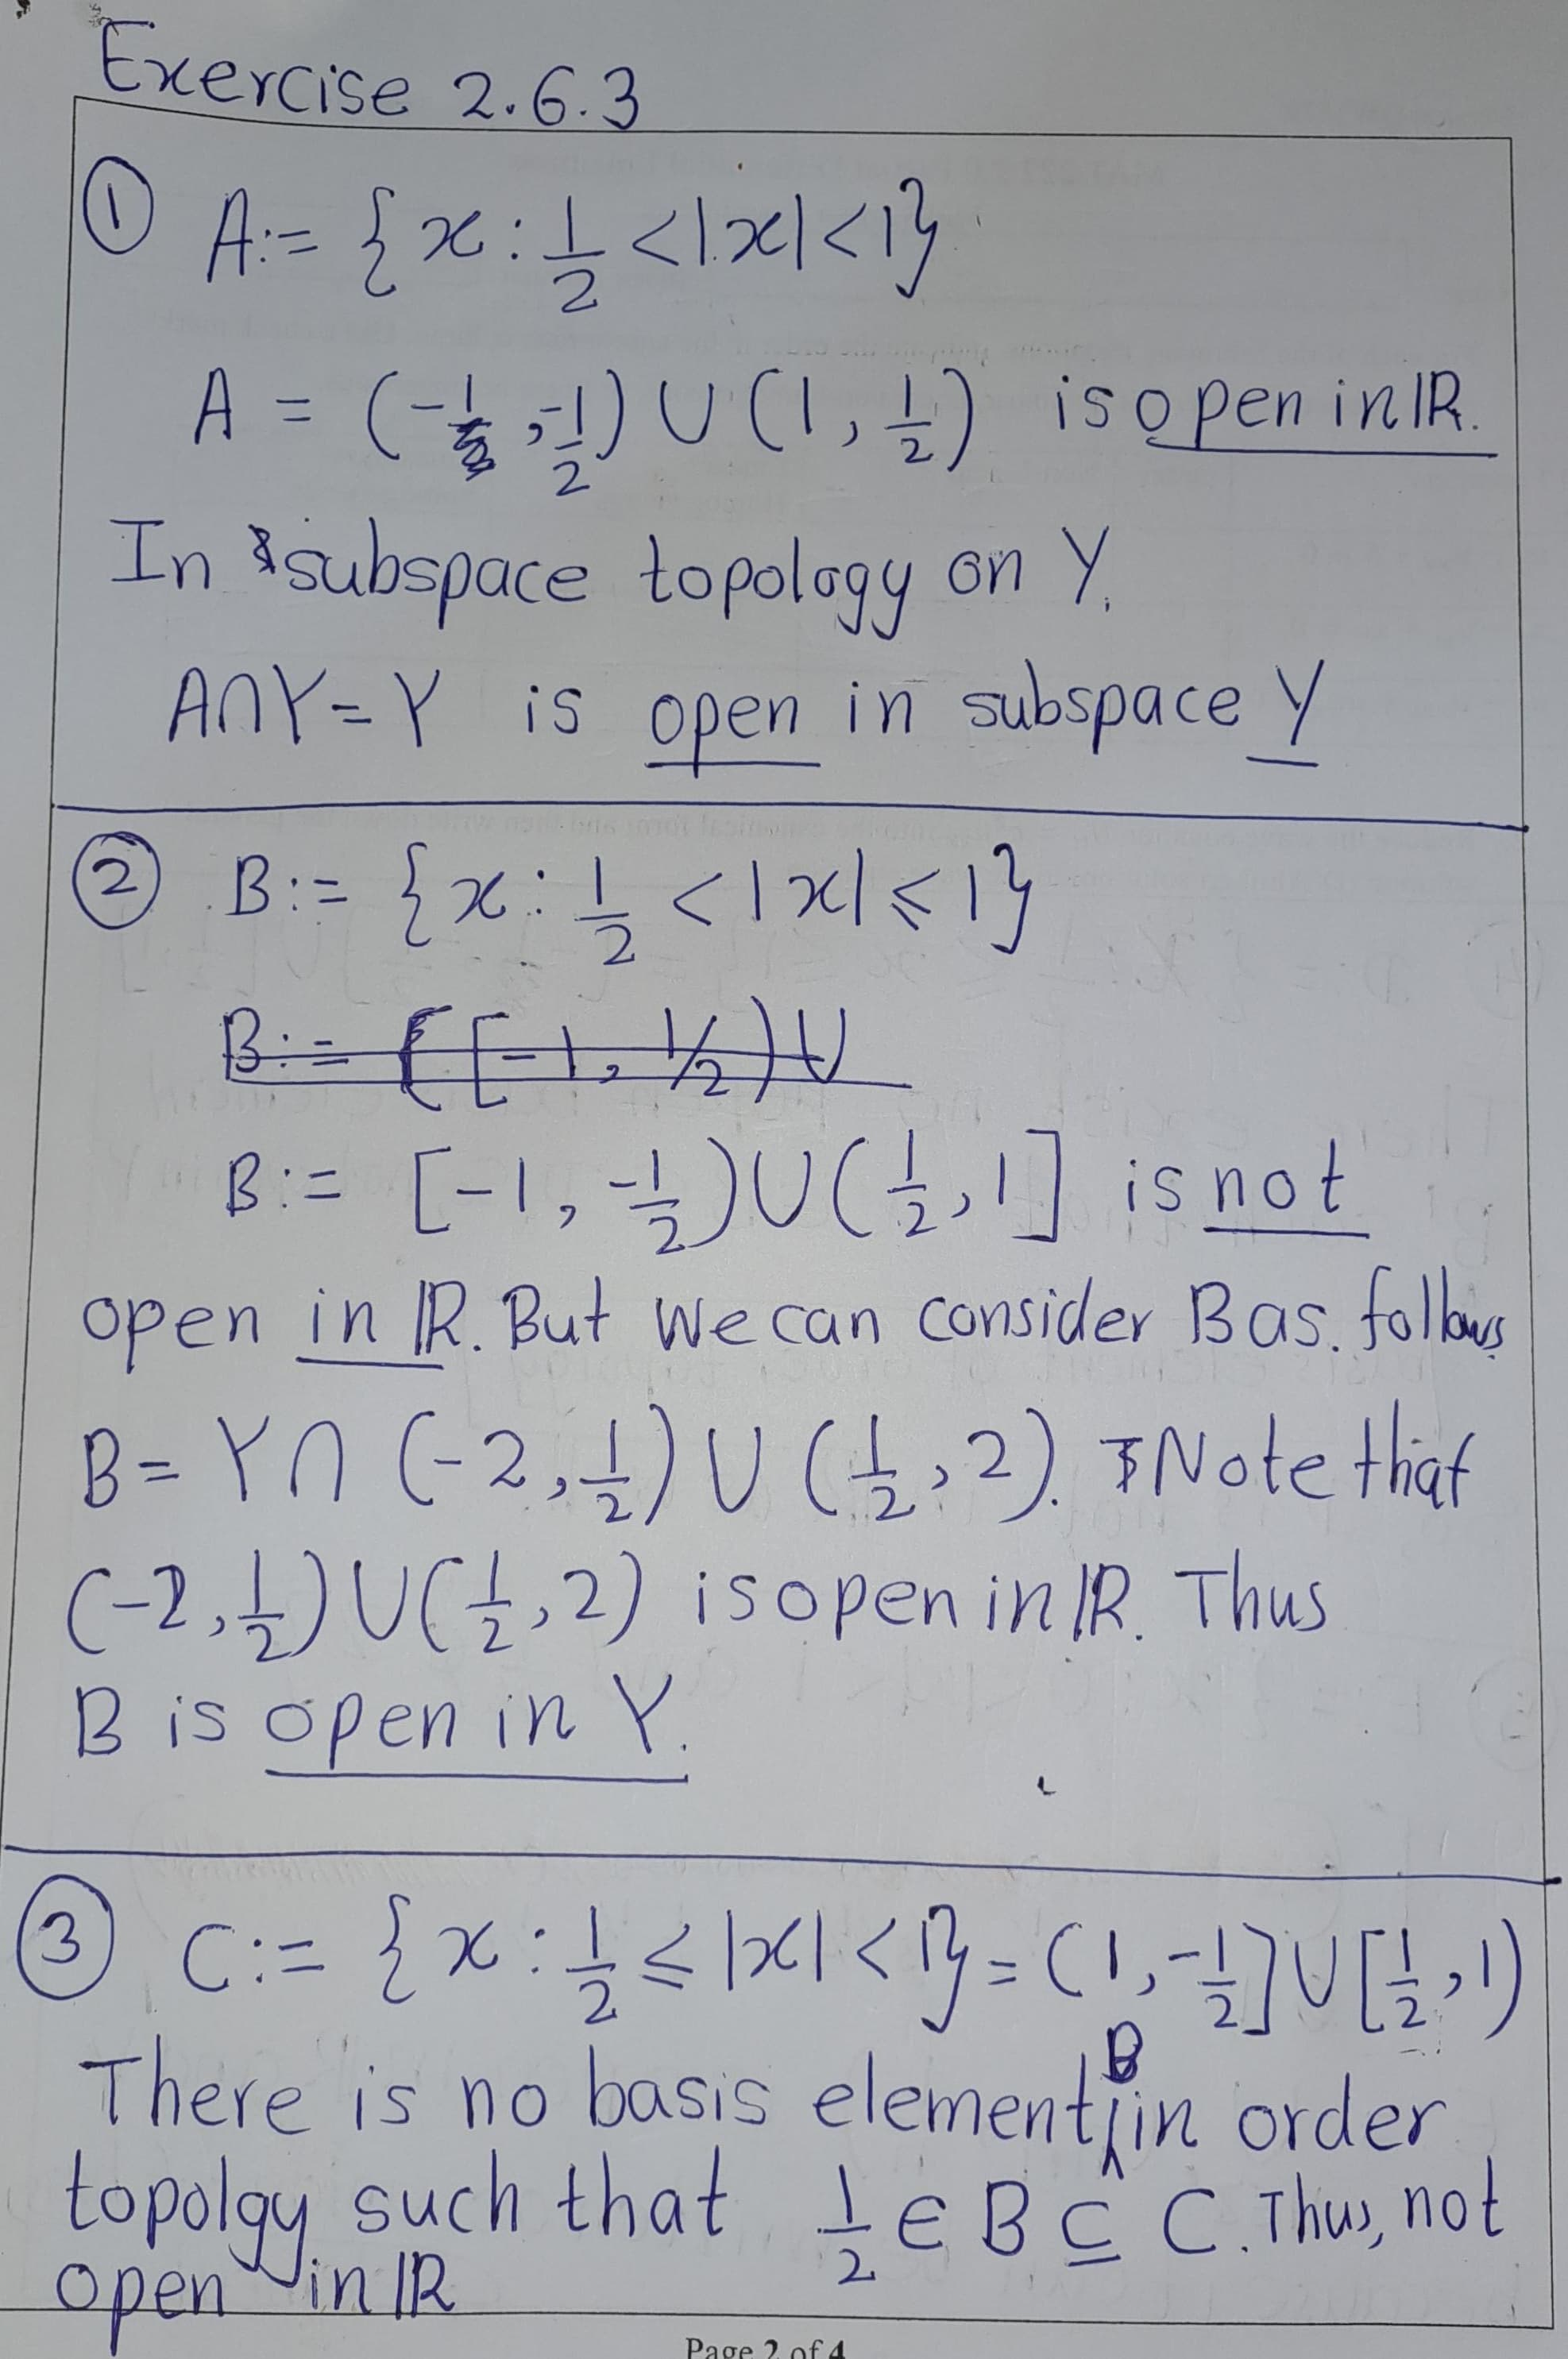
\includegraphics{figures/Exercises/Ex 2.16/ex-3-1.jpg}

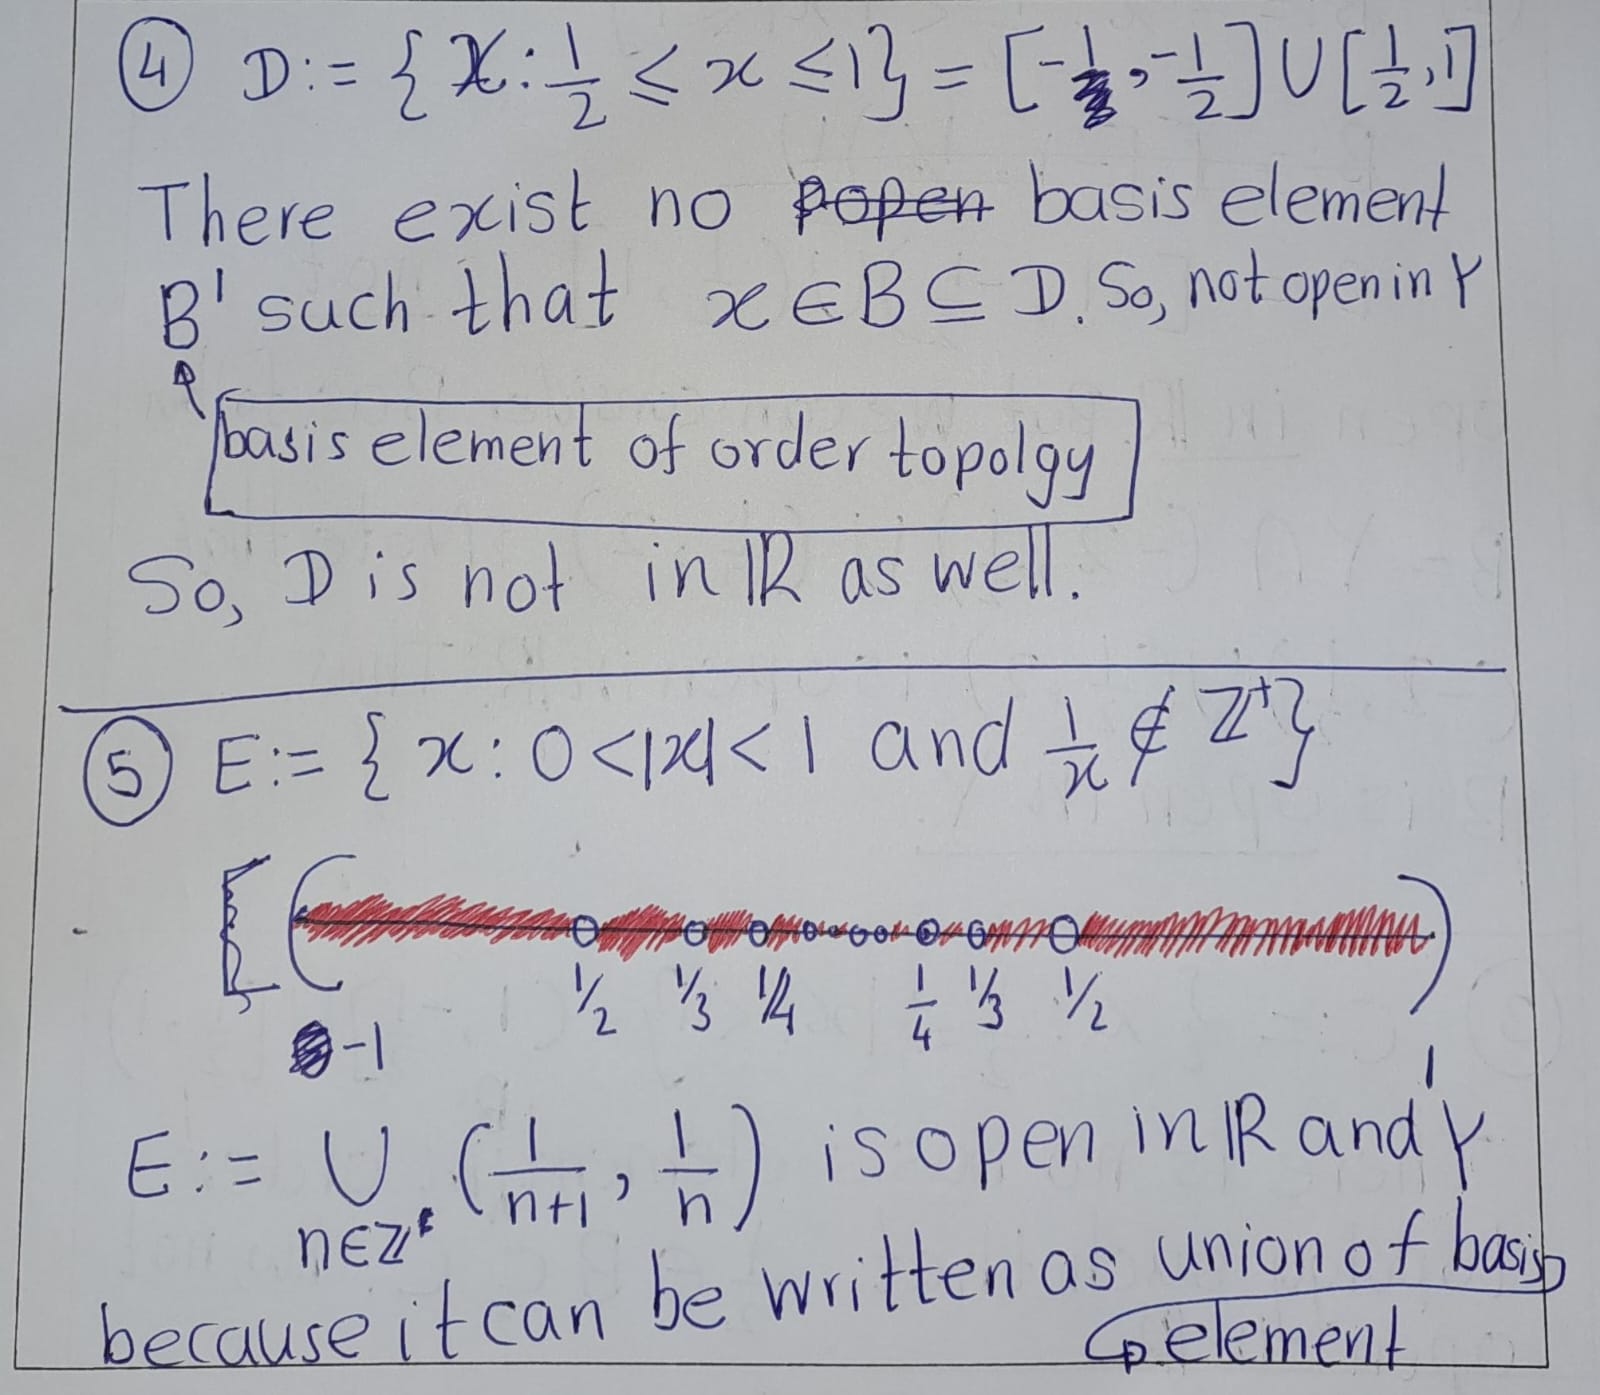
\includegraphics{figures/Exercises/Ex 2.16/ex-3-2.jpg}

\begin{exercise}
\protect\hypertarget{exr:unnamed-chunk-121}{}\label{exr:unnamed-chunk-121}A map \(f : X \to Y\). We say that \(f\) is an \textbf{open map} if, for every open set \(U\) in \(X\), the set \(f(U)\) is open in \(Y\). Show that the projections \(\pi_1 : X \times Y \to X\) and \(\pi_2 : X \times Y \to Y\) are open maps.
``
\end{exercise}

\begin{exercise}
\protect\hypertarget{exr:unnamed-chunk-122}{}\label{exr:unnamed-chunk-122}

Let \(X\) and \(X^\prime\) denote a single set in the topologies \(\mathcal{T}\) and \(\mathcal{T}^\prime\) , respectively; let \(Y\)
and \(Y'\) denote a single set in the topologies \(\mathcal{U}\) and \(\mathcal{U}^\prime\), respectively. Assume these sets are nonempty.

\begin{enumerate}
\def\labelenumi{(\alph{enumi})}
\tightlist
\item
  Show that if \(\mathcal{T}' \supset \mathcal{T}\) and \(\mathcal{U}'\supset \mathcal{U}\), then the product topology on \(X'\times Y'\) is
  finer than the product topology on \(X \times Y\).
\item
  Does the converse of a. hold? Justify your answer
\end{enumerate}

\end{exercise}

\begin{exercise}[Mun 2.16.7]
\protect\hypertarget{exr:unnamed-chunk-123}{}\label{exr:unnamed-chunk-123}Show that the countable collection
\[\{(a, b) \times (c, d) | a < b \text{ and } c < d, \text{ and } a, b, c, d \text{ are rational}\}\]
is a basis for \(\mathbb{R}^2\).''
\end{exercise}

\begin{exercise}
\protect\hypertarget{exr:unnamed-chunk-124}{}\label{exr:unnamed-chunk-124}Let \(X\) be an ordered set. If \(Y\) is a proper subset of \(X\) that is convex in \(X\), does it follow that \(Y\) is an interval or a ray in \(X\)?
\end{exercise}

\begin{exercise}
\protect\hypertarget{exr:unnamed-chunk-125}{}\label{exr:unnamed-chunk-125}If \(L\) is a straight line in the plane, describe the topology \(L\) inherits as a subspace of \(\mathbb{R}_l \times \mathbb{R}\) and as a subspace of \(\mathbb{R}_l \times \mathbb{R}_l\). In each case it is a familiar topology.
\end{exercise}

\begin{exercise}
\protect\hypertarget{exr:unnamed-chunk-126}{}\label{exr:unnamed-chunk-126}Show that the dictionary order topology on the set \(\mathbb{R} \times \mathbb{R}\) is the same as the product topology \(\mathbb{R}_d \times \mathbb{R}\), where \(\mathbb{R}_d\) denotes \(\mathbb{R}\) in the discrete topology. Compare this topology with the standard topology on \(\mathbb{R}^2\).
\end{exercise}

\[\mathbb{R}^2_{dictionary}:=\mathbb{R}_{discrete }\times \mathbb{R}_{standard}\]

\begin{proof}
Let \(\{a\} \times (c,d)\) be a basis element in product toplogy \(\mathbb{R}_d \times \mathbb{R}\). Let \(a\times x\in \{a\} \times (c,d)\) obsereve that
\[a\times x\in \{a\} \times (c,d) = (a\times c,a\times d)\]
and \((a\times c,a\times d)\) is basis element of order topology \(\mathbb{R}^2\). Thus by lemma \ref{lem:finerLemma}, order toplogy in \(\mathbb{R}^2\) is finer than the product toplogy \(\mathbb{R}_d \times \mathbb{R}\).

Now suppose that \((p\times q, r \times s)\) be a basis elemenet in order toplogy on \(\mathbb{R}^2\).

\begin{itemize}
\tightlist
\item
  If \(p<x\), define \(l=y−1\) and if \(p=x\) define \(l=r\). In either case we know that \((p\times q)<(x\times l)<(x\times y)\).
\item
  If \(x<r\) define \(t=y+1\) and if \(x=r\) define \(t=s\). In either case we know that \((x\times y)<(x\times t)<(q \times s)\).
\end{itemize}

See figure \ref{fig:fig12}
So \[(x,y) \in \{x\} \times (l,t) \subseteq (p \times q, r \times s).\]
Thus by lemma \ref{lem:finerLemma}, product toplogy \(\mathbb{R}_d \times \mathbb{R}\) is finer than order toplogy in \(\mathbb{R}^2\).

Therefore, \[\mathbb{R}^2_{dictionary}=\mathbb{R}_{discrete }\times \mathbb{R}_{standard}\]
\end{proof}

\begin{figure}
\centering
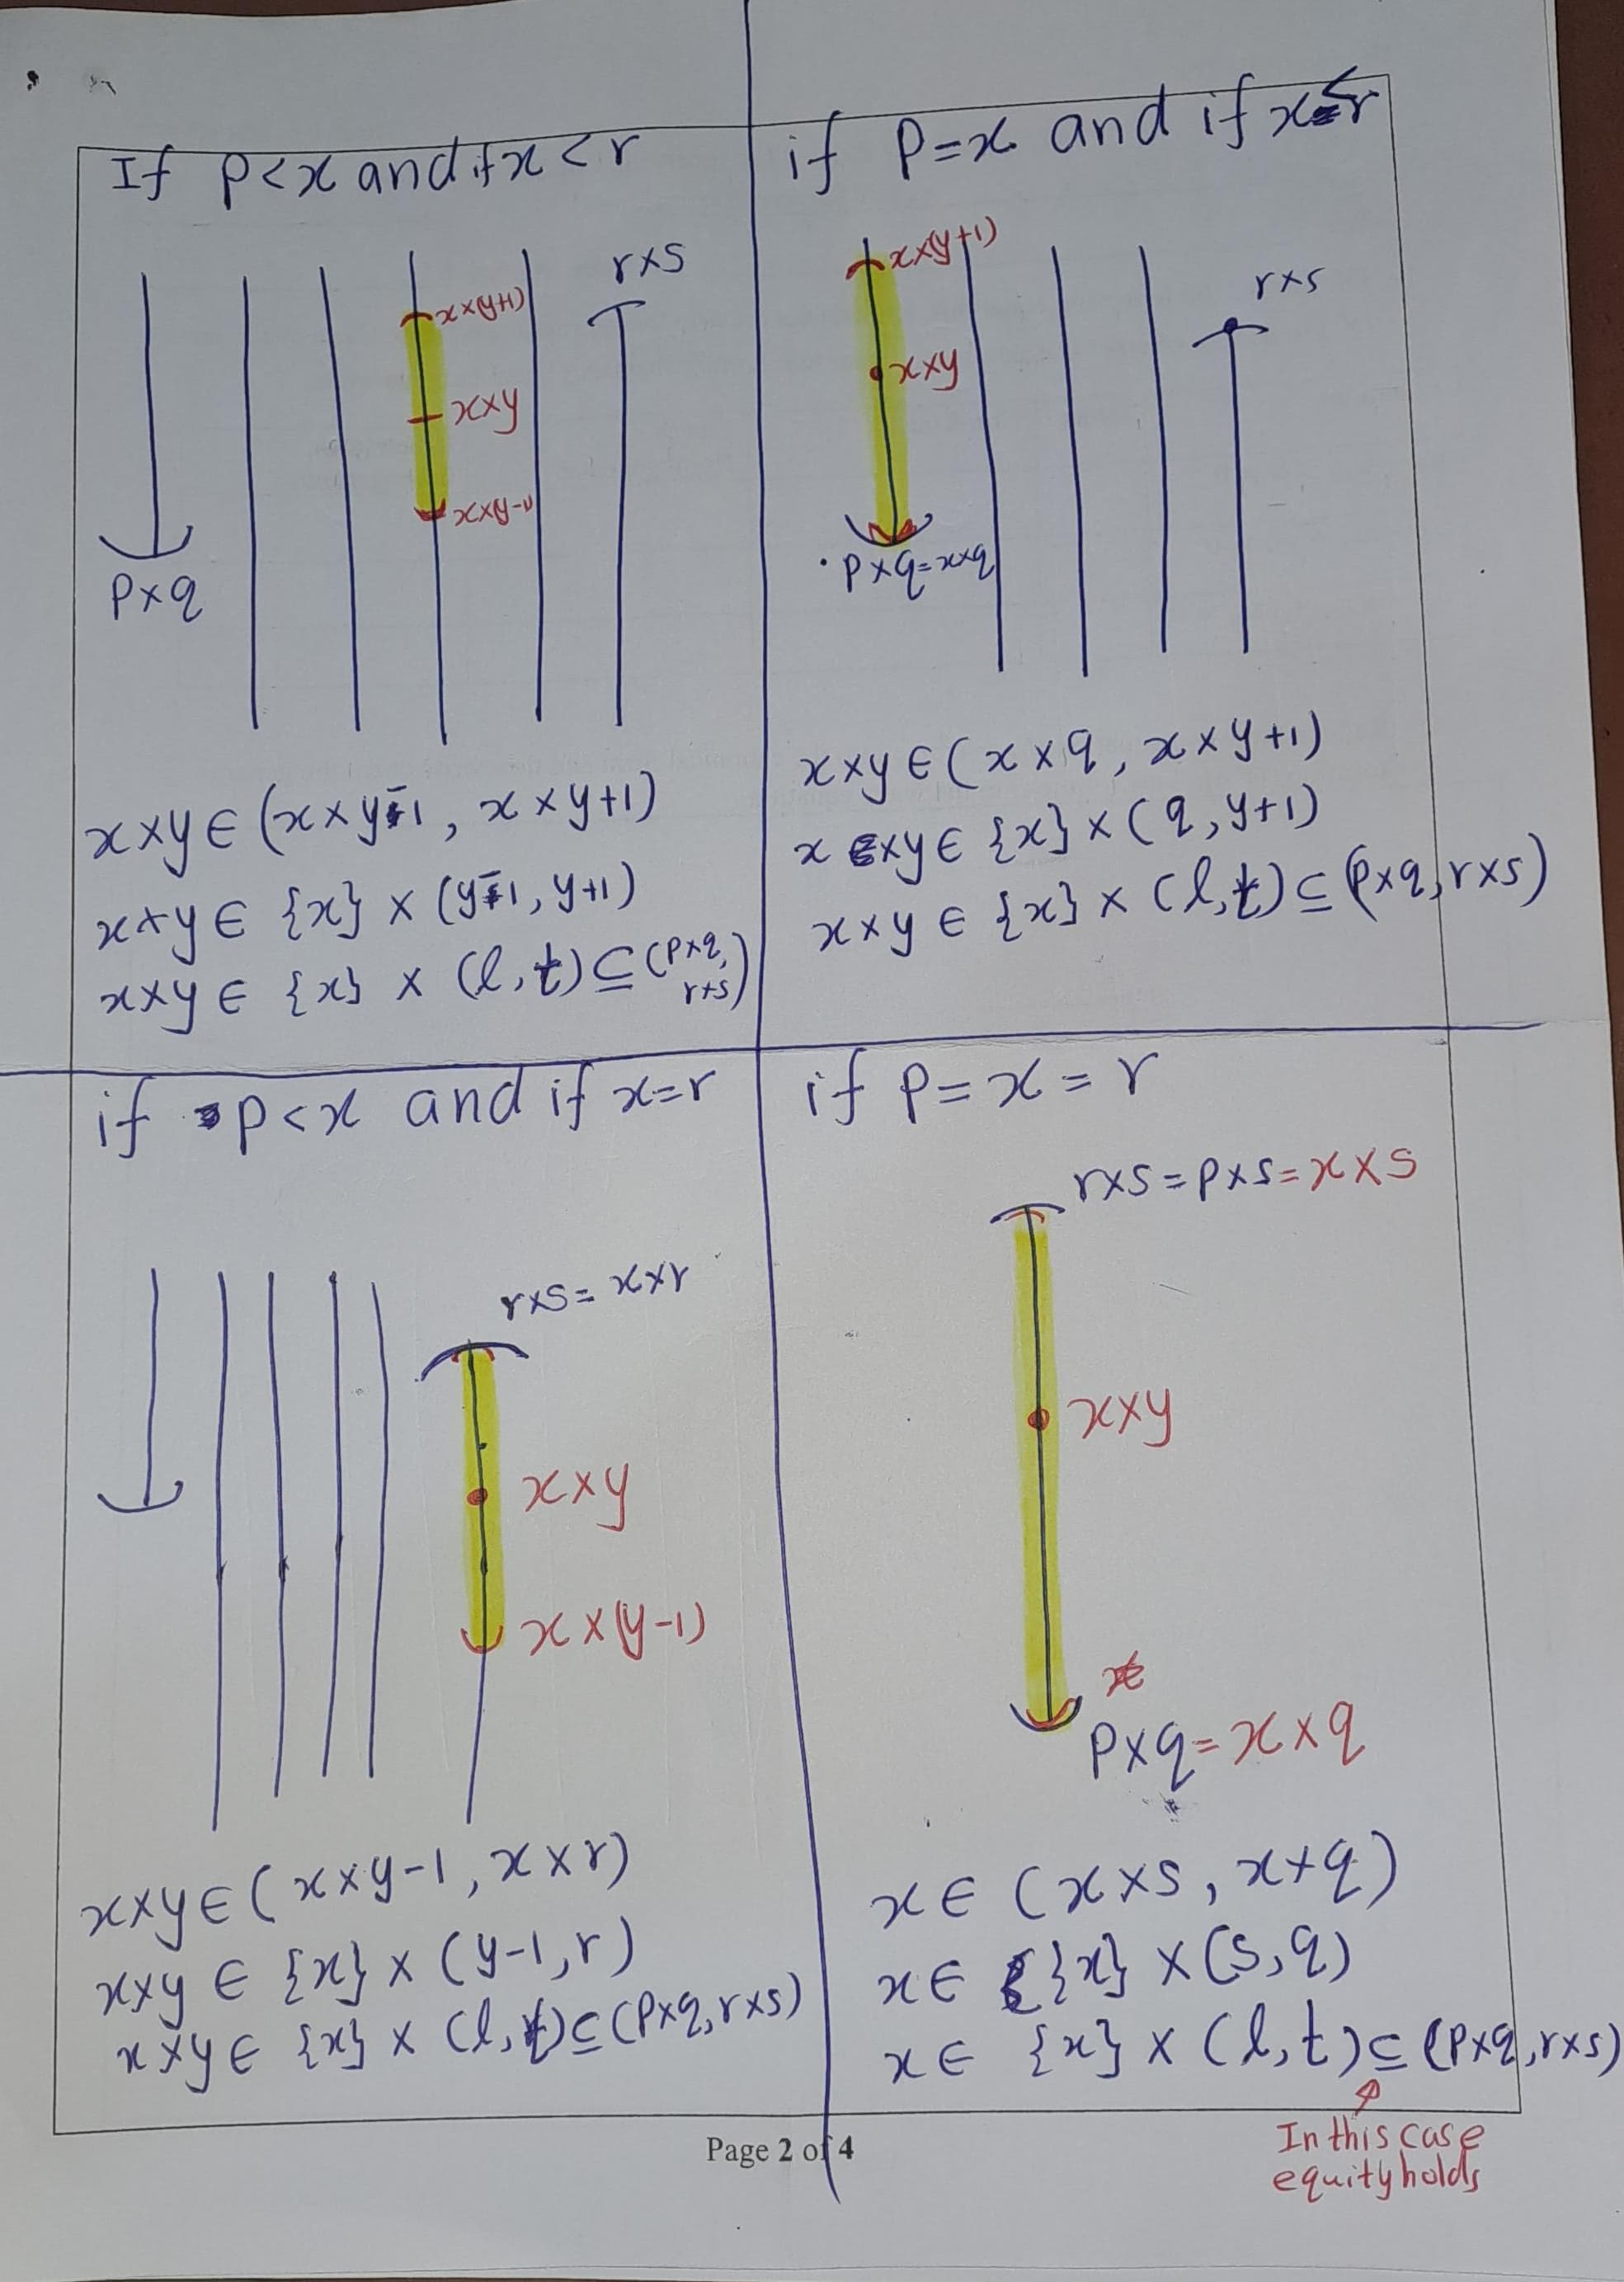
\includegraphics{figures/figure 12.jpg}
\caption{\label{fig:figm12}\(~\)}
\end{figure}

Let \(I = [0, 1]\). Compare the product topology on \(I \times I\), the dictionary order topology on \(I \times I\), and the topology \(I \times I\) inherits as a subspace of \(\mathbb{R} \times \mathbb{R}\) in the dictionary order topology.

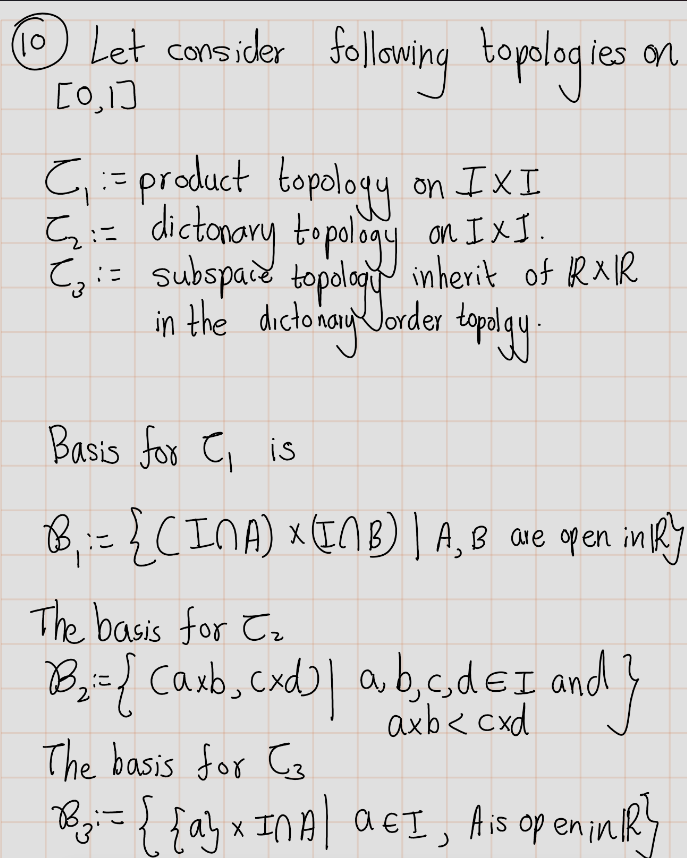
\includegraphics{figures/Exercises/Ex 2.16/ex-10-1.png}
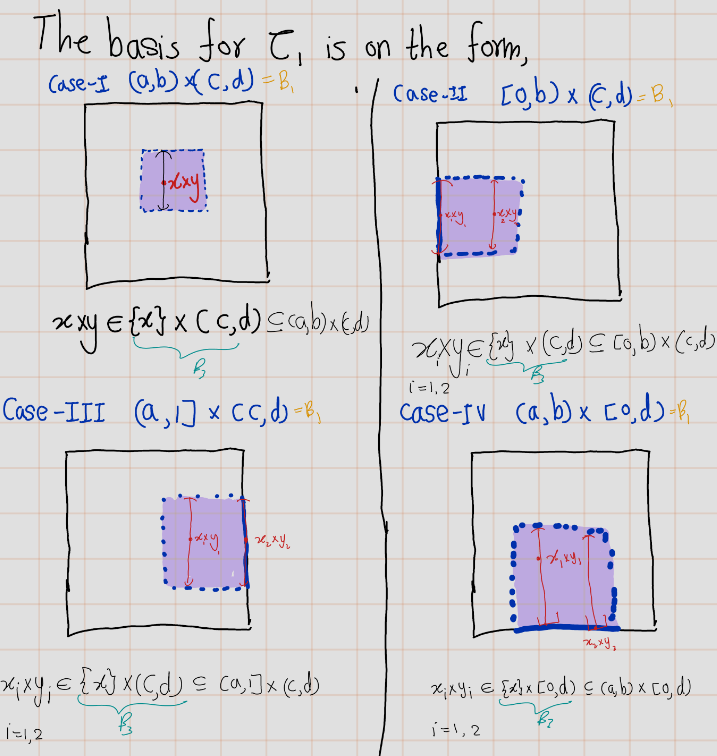
\includegraphics{figures/Exercises/Ex 2.16/ex-10-2.png}
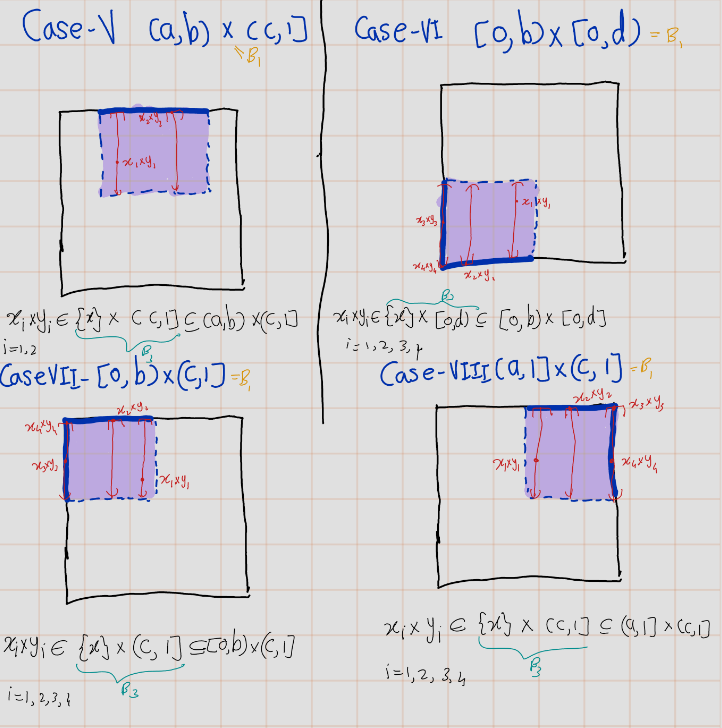
\includegraphics{figures/Exercises/Ex 2.16/ex-10-3.png}
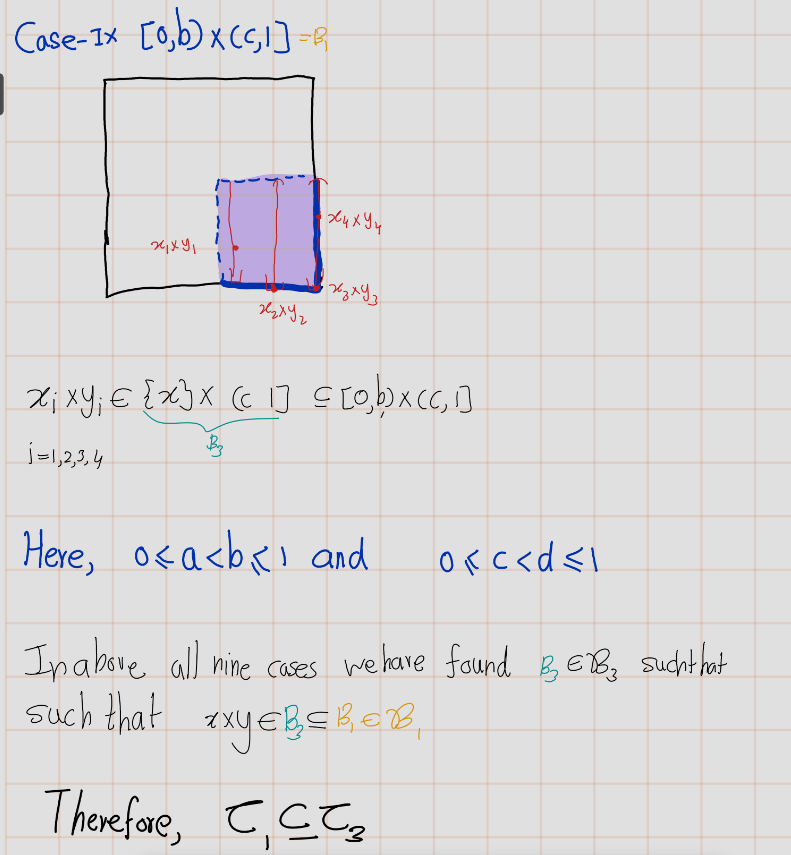
\includegraphics{figures/Exercises/Ex 2.16/ex-10-4.png}
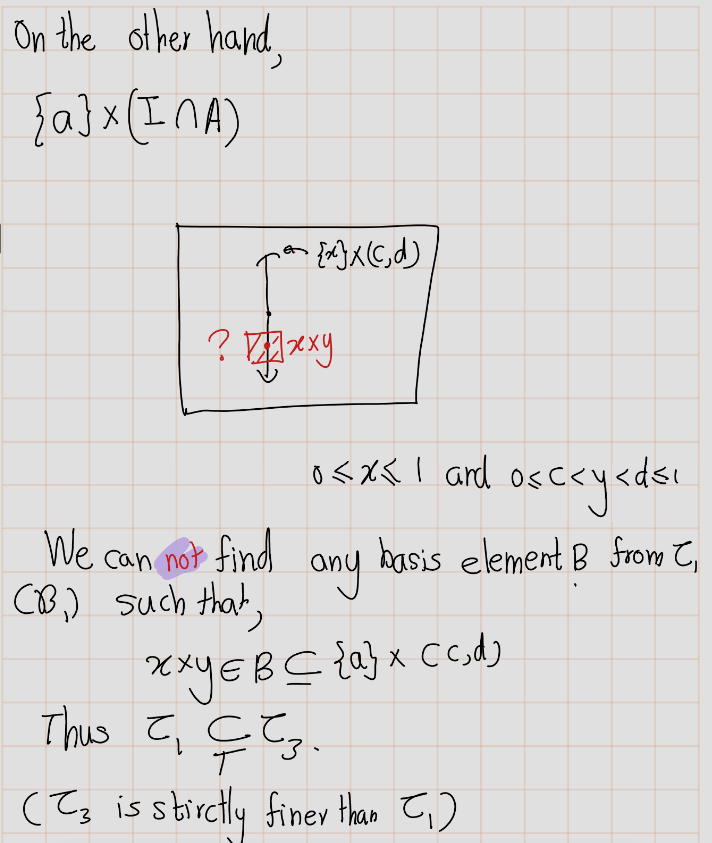
\includegraphics{figures/Exercises/Ex 2.16/ex-10-5.png}

\textbf{Claim}: \(\mathcal{T_2}\subsetneq\mathcal{T3}\)\\
So, as previous we have to prove two things they are finer condition and strictly condition.

Let \((a_1\times b_1, a_2 \times b_2)\) be a basis element of order topology. and \(x\times y \in (a_1\times b_1, a_2 \times b_2)\)

\begin{itemize}
\item
  \textbf{Case I} \((a_1<x<a_2)\):
  \[x\times y \in (x\times-1,x\times 2)\cap I^2= [x\times 0,x\times 1]=\{x\}\times [0,1] \subset (a_1\times b_1, a_2 \times b_2)\]
  Note that \((x\times -1,x\times 2)\cap I^2\) is a basis element of subspace topology.
\item
  \textbf{Case II} \((a_1=x<a_2)\):
  \[x\times y \in (x\times b_1,x\times 2)\cap I^2= [x\times b_1,x\times 1]=\{x\}\times (b_1,1] \subset (a_1\times b_1, a_2 \times b_2)\]
  Note that \((x\times b_1,x\times 2)\cap I^2\) is a basis element of subspace topology.
\item
  \textbf{Case III} \((a_1<x=a_2)\):
  \[x\times y \in (x\times -1,x\times b_2)\cap I^2= [x\times 0,x\times b_2]=\{x\}\times [0,b_2) \subset (a_1\times b_1, a_2 \times b_2)\]
  Note that \((x\times -1,x\times b_2)\cap I^2\) is a basis element of subspace topology.
\item
  \textbf{Case IV} \((a_1=x=a_2)\):
  \[x\times y \in (x\times b_1,x\times b_2)\cap I^2= [x\times b_1,x\times b_2]=\{x\}\times [b_1,b_2) \subset (a_1\times b_1, a_2 \times b_2)\]
  Note that \((x\times b_1,x\times b_2)\cap I^2\) is a basis element of subspace topology.
\end{itemize}

See figure \ref{fig:fige15}

In above all four cases, we have found basis element of subspace topology that contain \(x\times y\) and contained in \((a_1\times b_1, a_2 \times b_2)\). Therefore, \(\mathcal{T_2}\subsetneq\mathcal{T3}\)

\begin{figure}
\centering
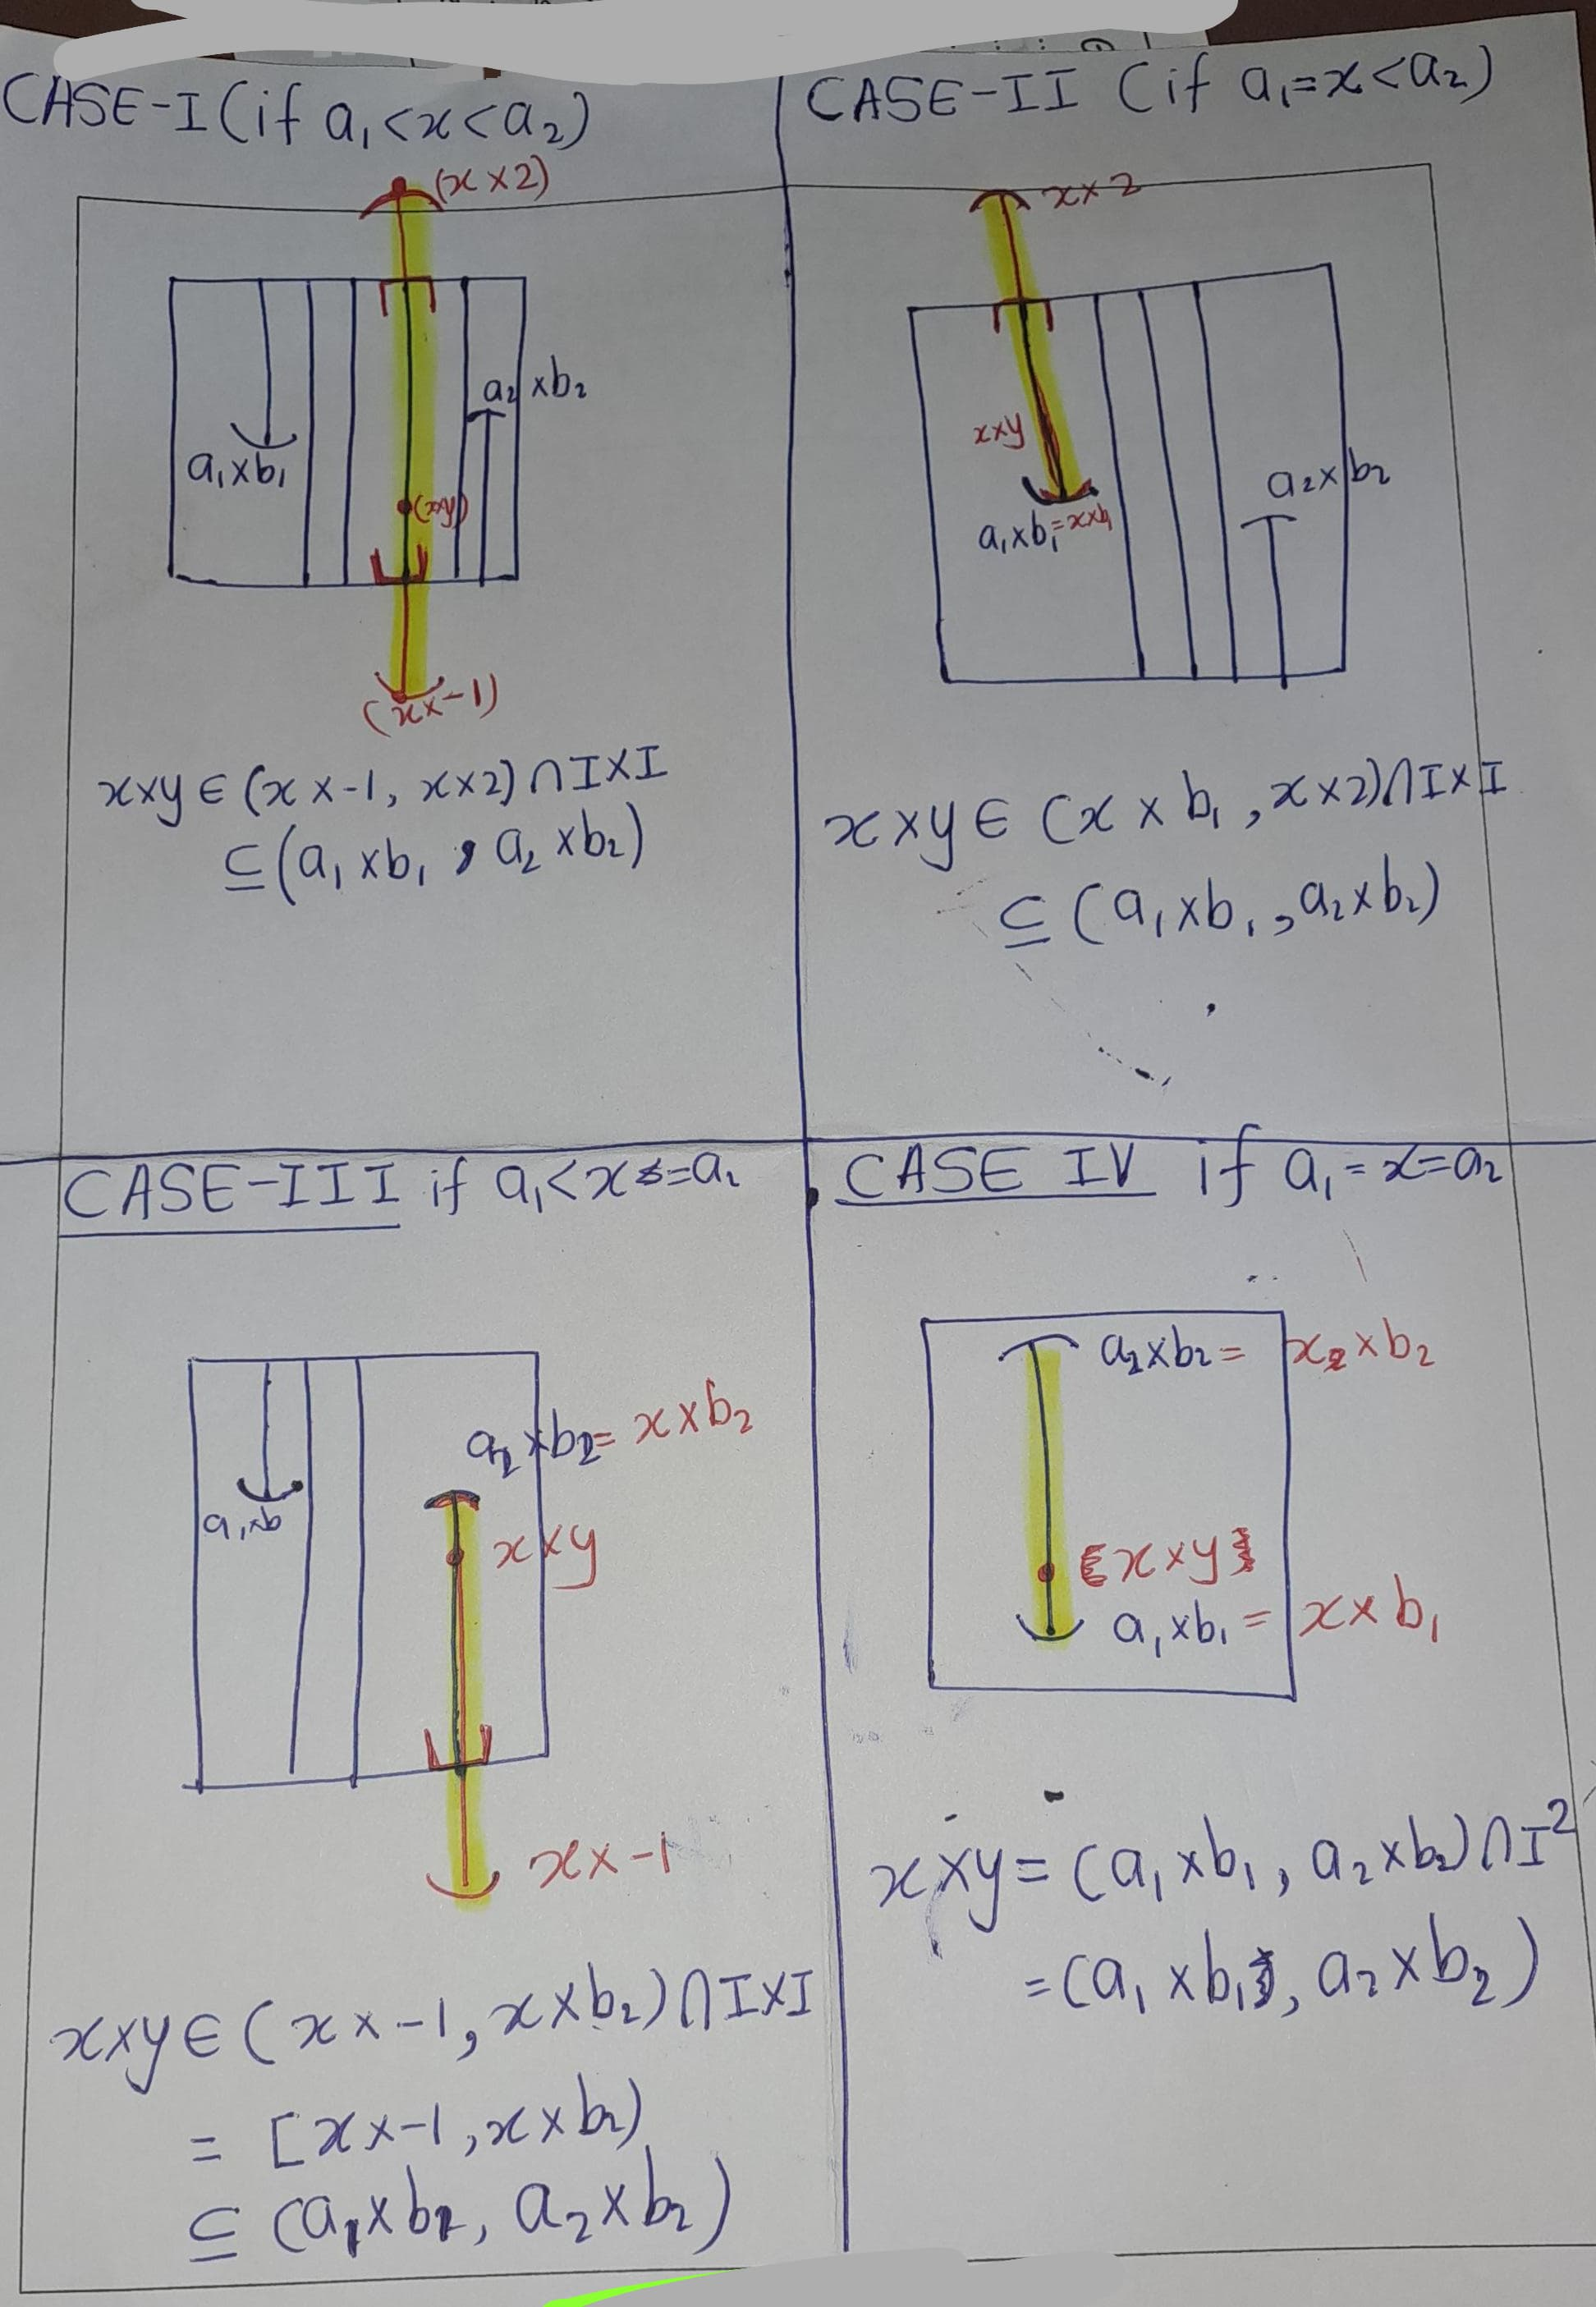
\includegraphics{figures/figure 15.jpg}
\caption{\label{fig:fige15}\(~\)}
\end{figure}

\begin{center}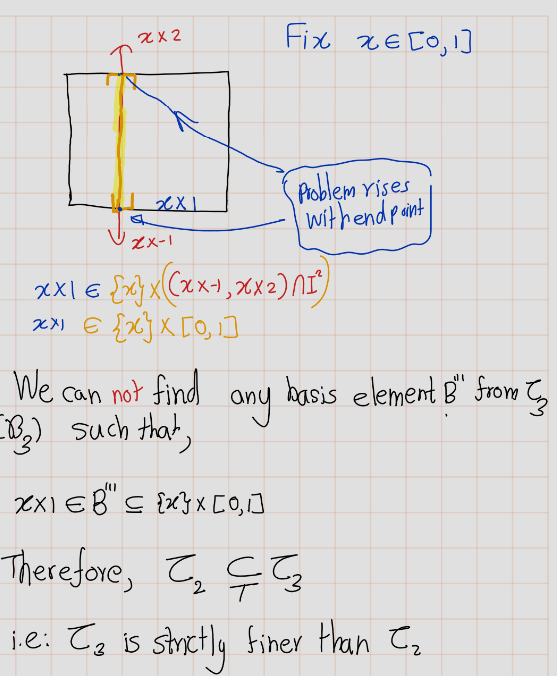
\includegraphics{figures/Exercises/Ex 2.16/ex-10-6} \end{center}

\begin{center}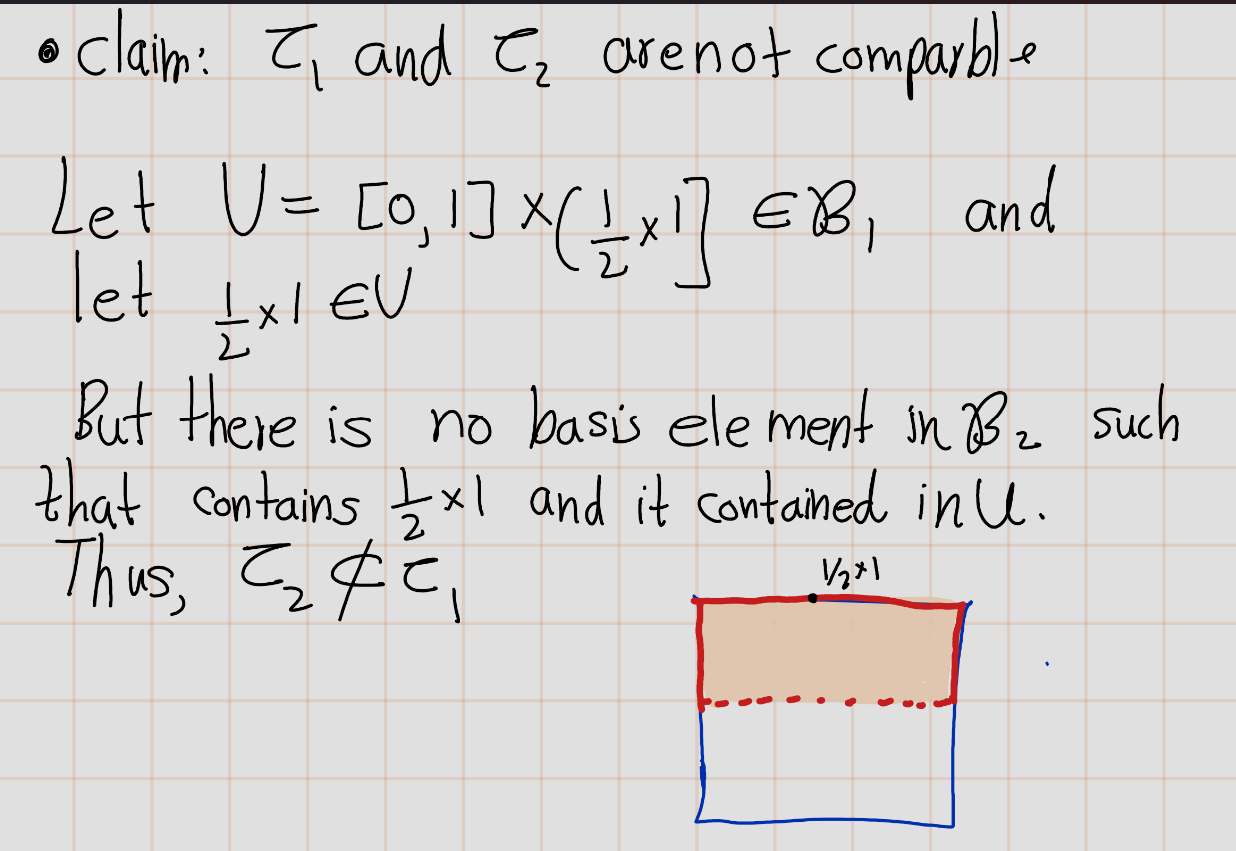
\includegraphics{figures/Exercises/Ex 2.16/ex-10-7} \end{center}

\begin{center}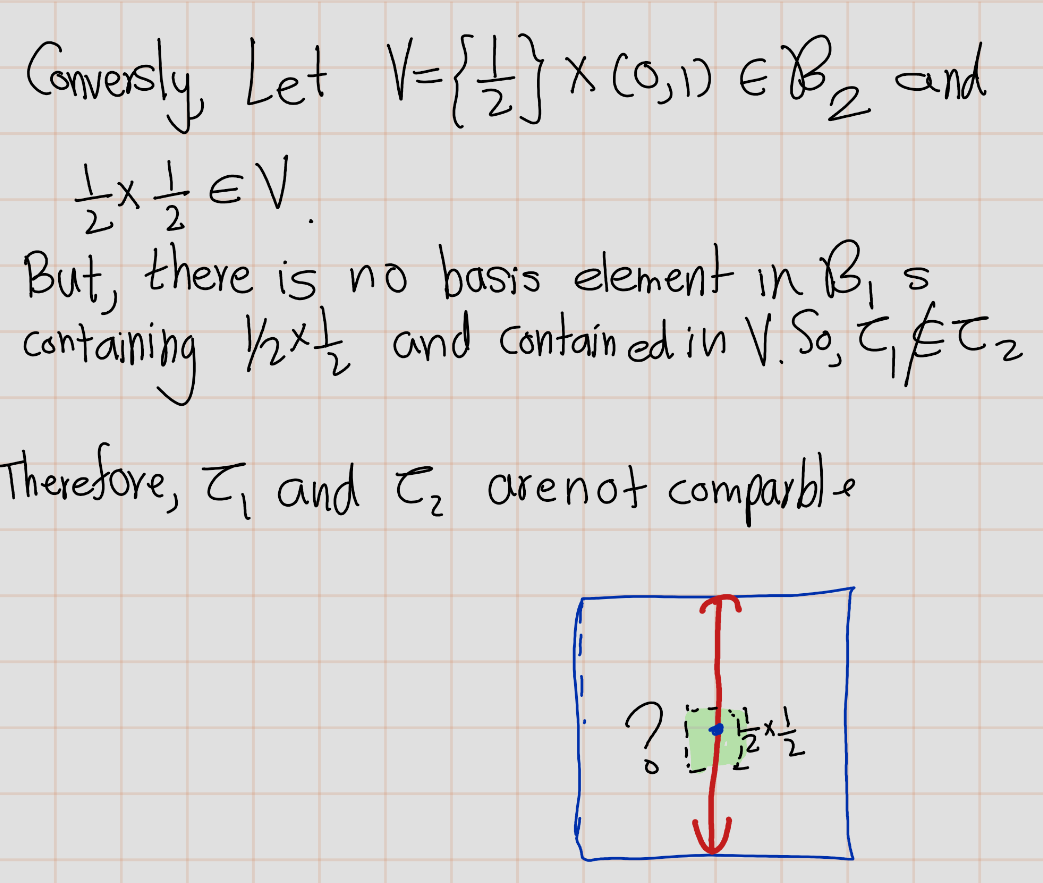
\includegraphics{figures/Exercises/Ex 2.16/ex-10-8} \end{center}

\hypertarget{section-17-in-munkress-book}{%
\section{Section 17 in Munkress Book}\label{section-17-in-munkress-book}}

\begin{exercise}[Mun 2.17.1]
\protect\hypertarget{exr:unnamed-chunk-128}{}\label{exr:unnamed-chunk-128}Let \(\mathcal{C}\) be a collection of subsets of the set \(X\). Suppose that \$\$\emptyset and \(X\) are in \(\mathcal{C}\), and that finite unions and arbitrary intersections of elements of \(\mathcal{C}\) are in \(\mathcal{C}\). Show that the collection
\[\mathcal{T} = \{X \setminus C  | C\in  \mathcal{C}\}\]
is a topology on X.
\end{exercise}

\textbf{Solution}:

\begin{proof}
\leavevmode

\begin{itemize}
\tightlist
\item
  (T1)

  \begin{itemize}
  \tightlist
  \item
    \(\emptyset \in \mathcal{C}\implies X\setminus \emptyset=X \in \mathcal{T}\).
  \item
    \(X \in \mathcal{C}\implies X\setminus X=\emptyset \in \mathcal{T}\)
  \end{itemize}
\item
  (T2)
  Let \(\{U_\alpha\}_{\alpha\in J}\) be family of elements in \(\mathcal{C}\). Then \((X\setminus U_\alpha\}_{\alpha\in J}\in \mathcal{T}\). Then,
  \[\bigcup_{\alpha\in J}(X\setminus U_\alpha)=X\setminus \bigcup_{\alpha\in J}U_\alpha\]
  Since \(\mathcal{C}\) is closed arbitrary intersection, \(\bigcup_{\alpha\in J}\in \mathcal{C}\). Thus,\(\bigcap_{\alpha\in J}(X\setminus U_\alpha)=X\setminus \bigcup_{\alpha\in J}U_\alpha\in \mathcal{T}\).
\item
  (T3)
  Let \(U_1,U_2,...,U_n\in \mathcal{C}\). Then \((X\setminus U_1),(X\setminus U_2),...,(X\setminus U_n)\in \mathcal{T}\). Then,
  \[\bigcap_{i=1}^n(X\setminus U_i)=X\setminus \bigcup_{i=1}^nU_i\]
  Since \(\mathcal{C}\) is closed under finite union, \(\bigcup_{i=1}^nU_i\in \mathcal{C}\). Thus,\(\bigcap_{i=1}^n(X\setminus U_i)=X\setminus \bigcup_{i=1}^nU_i\in \mathcal{T}\).
  Therefore \(\mathcal{T}\) is a topology on \(X\).
\end{itemize}

\end{proof}

\begin{exercise}[Mun 2.17.2]
\protect\hypertarget{exr:unnamed-chunk-130}{}\label{exr:unnamed-chunk-130}Show that if \(A\) is closed in \(Y\) and \(Y\) is closed in \(X\), then \(A\) is closed in \(X\).
\end{exercise}

\begin{proof}
Since \(Y\) is subspace in \(X\) and \(A\) is closed in \(Y\), by theorm \ref{thm:qw}, then there exist closed set \(C\) in \(X\) such that \[A=Y\cap C\]
Since, \(Y\) is closed in \(X\) and \(X\) is toplogical space, \(A=Y\cap C\) is closed in \(X\).
\end{proof}

\begin{exercise}[Mun 2.17.3]
\protect\hypertarget{exr:unnamed-chunk-132}{}\label{exr:unnamed-chunk-132}Show that if \(A\) is closed in \(X\) and \(B\) is closed in \(Y\) , then \(A\times B\) is closed in \(X\times Y\)
\end{exercise}

\begin{proof}
Suppose that \(A\) is closed in \(X\) and \(B\) is closed in \(Y\). Then \(X\setminus A\) is open in \(X\) and \(X\setminus B\) is open in \(Y\).

\textbf{Claim}: \((X\times Y) \setminus (A\times B)=  ((X\setminus A)\times Y)\cup((X\times (Y\setminus B)))\)\\
\emph{Proof of Claim}:
\begin{eqnarray}
(x\times y)\in (X\times Y) \setminus (A\times B) 
&\iff & (x\times y)\not\in (A\times B)\\
&\iff & x\not\in A \text{ or } y \not\in B\\
&\iff & x\in X\setminus A \text{ or } y \in Y\setminus B\\
&\iff& (x\times y) \in ((X\setminus A)\times Y)\cup((X\times (Y\setminus B)))
\end{eqnarray}
So, now we are done proof of the claim.
Thus, \((X\times Y) \setminus (A\times B)\) is union of open sets and hence, \((X\times Y) \setminus (A\times B)\) is open in \(X \times Y\). Thus, \((A\times B)\) is closed in \(X\times Y\).
\end{proof}

\begin{exercise}[Mun 2.17.4]
\protect\hypertarget{exr:unnamed-chunk-134}{}\label{exr:unnamed-chunk-134}Show that if \(U\) is open in \(X\) and \(A\) is closed in \(X\), then \(U \setminus A\) is open in \(X\), and \(A \setminus U\) is closed in \(X\).
\end{exercise}

\begin{proof}
Suppose that \(U\) is open in \(X\) and \(A\) is closed in \(X\).

\textbf{Claim 1}: \((U\setminus A)=U\cap (X\setminus A)\).\\
\begin{eqnarray}
x \in (U\setminus A)
&\iff& x\in U \text{ and } x\not\in A\\
&\iff& x\in U  \text{ and } x\in X\setminus A\\
&\iff& x\in U  \cap X\setminus A\\
\end{eqnarray}
Since, \(A\) is closed in \(X\), \(X\setminus A\) is open in \(X\). Thus, \((U\setminus A)=U\cap (X\setminus A)\) is open in \(X\). (By finite intersection property.)

\textbf{Claim 2}: \((A\setminus U)=A\cap (X\setminus U)\).\\
Similar to proof of claim 1 we can prove this claim.

Since, \(U\) is open in \(X\), \(X\setminus U\) is closed in \(X\). Thus, \((A\setminus U)=A\cap (X\setminus U)\) is closed in \(X\).
\end{proof}

\begin{exercise}[Mun 2.17.5]
\protect\hypertarget{exr:unnamed-chunk-136}{}\label{exr:unnamed-chunk-136}Let \(X\) be an ordered set in the order topology. Show that \(\overline{(a, b)} \subseteq [a, b]\). Under what conditions does equality hold?
\end{exercise}

\begin{proof}
\emph{(Proof of \(\overline{(a, b)} \subseteq [a, b]\))}

\textbf{Claim 1}: \([a,b]\) is closed in \(X\) under order toplology.\\
Observe that,
\[X\setminus[a,b] =(-\infty,a)\cup (b,\infty).\]
Note that, \((-\infty,a)\) and \((b,\infty)\) are open rays.
Then \((-\infty,a)\cup (b,\infty)=X\setminus [a,b]\) is open.
Thus, \([a,b]\) is closed in \(X\) under order toplogy.

\textbf{Claim 2}: \((a,b)\subseteq [a,b]\)\\
Now, let \(x \in (a, b)\) then \(a < x < b\) so clearly \(a \leq x \leq b\) so \(x\) is in \([a, b]\). Thus \((a,b)\subseteq [a,b]\).

Therefore, by cliam 1 and 2, \([a, b]\) is a closed set containing \((a, b)\).

Now, to show \(\overline{(a, b)} \subseteq [a, b]\), recall that \(\overline{(a, b)}\) is the intersection of all closed sets containing \((a, b)\).
Let \(x \in \overline{(a, b)}\) Since, \(x\) is in every closed set containing \((a, b)\) and \([a, b]\) is a closed set containing \((a, b)\),then \(x \in [a, b]\) as needed.

Let \(a^{+} = \inf\{x : x > a\}\) and let \(b^{-} = \sup\{x : x < b\}\). Consider the closed set \([x, y]\). If \([x, y]\) contains
\((a, b)\), then \(x \leq a^{+}\) and \(y \geq b^{-}\). Thus there exists a closed set containing \((a, b)\) that does not contain
\(a\) or \(b\) if and only if \(a^{+} \neq a\) or \(b^{-} \neq b\). This is true exactly when \(a\) has an immediate successor or \(b\)
has an immediate predecessor.
\end{proof}

\begin{itemize}
\tightlist
\item
  For example, in the order topology on \(\mathbb{Z}\), \[\overline{(1, 4)} = [2, 3] \subsetneq [1, 4].\]
\end{itemize}

\begin{exercise}[Mun 2.17.6]
\protect\hypertarget{exr:unnamed-chunk-138}{}\label{exr:unnamed-chunk-138}

Let \(A\), \(B\), and \(A_{\alpha}\) denote subsets of a space \(X\). Prove the following:

\begin{enumerate}
\def\labelenumi{(\alph{enumi})}
\tightlist
\item
  If \(A \subset B\), then \(\overline{A} \subset \overline{B}\).
\item
  \(\overline{A \cup B} = \overline{\overline{A}} \cup \overline{\overline{B}}\).
\item
  \(\overline{\bigcup A_{\alpha}} \supseteq \bigcup \overline{A_{\alpha}}\); give an example where equality fails.
\end{enumerate}

\end{exercise}

\begin{proof}

Let \(A\), \(B\), and \(A_{\alpha}\) denote subsets of a space \(X\).

\begin{enumerate}
\def\labelenumi{(\alph{enumi})}
\item
  By definition, \(\overline{A}\) is the intersection of all closed sets containing \(A\). Since \(\overline{B}\) is a closed set that contains \(B\) and hence \(A\), it must therefore contain \(\overline{A}\).
\item
\end{enumerate}

\begin{itemize}
\item
  \textbf{Claim 1}: \(\overline{A \cup B} \supseteq {\overline{A}} \cup {\overline{B}}\)\\
  The set \(\overline{A \cup B}\) is a closed set that contains \(A \cup B\), so it contains both \(A\) and \(B\),
  and therefore it contains both \(\overline{A}\) and \(\overline{B}\). Therefore, \(\overline{A \cup B} \supseteq {\overline{A}} \cup {\overline{B}}\).
\item
  \textbf{Claim 2}: \(\overline{A \cup B} \subseteq {\overline{A}} \cup {\overline{B}}\)\\
  \({\overline{A}} \cup \overline{B}\) is a closed set (since it is the union of two closed sets) that
  contains \(A \cup B\), (Beacuse \(A\subseteq\overline{A}\) and \(B \subseteq \overline{B}\implies A \cup B \subseteq \overline{A} \cup \overline{B}\).) so it contains \(\overline{A \cup B}\).
\end{itemize}

\begin{enumerate}
\def\labelenumi{(\alph{enumi})}
\setcounter{enumi}{2}
\tightlist
\item
  The set \(\overline{\bigcup A_{\alpha}}\) is a closed set that contains each \(A_{\alpha}\), so it contains each \(\overline{A_{\alpha}}\), and thus it contains \(\bigcup \overline{A_{\alpha}}\). Thus, \(\overline{\bigcup A_{\alpha}} \supseteq \bigcup \overline{A_{\alpha}}\)\\
  (But we can't do the converse because an arbitrary union of closures isn't necessarily closed!)\\
\end{enumerate}

\begin{itemize}
\tightlist
\item
  \textbf{Example 1 }that equality fails,\\
  Let \(A_n\) be the closed set \([\frac{1}{n}, 1] \subset \mathbb{R}\). Then \[\bigcup_{n \in \mathbb{N}} \overline{A_n} = \bigcup_{n \in \mathbb{N}} A_n =\bigcup_{n \in \mathbb{N}} [\frac{1}{n}, 1] = (0, 1], \text{ But } \bigcup_{n \in \mathbb{N}} A_n = [0, 1]\].
\item
  \textbf{Example 2 }that equality fails,\\
  Consider \(\mathbb{R}\) with the standard topology and all one-point sets \(\{q\}\) with \(q\) rational. Then \(\overline{\{q\}} = \{q\}\) for every such set, so that \(\bigcup_{q \in \mathbb{Q}} \overline{\{q\}} = \mathbb{Q}\), but \(\overline{\bigcup_{q \in \mathbb{Q}} \{q\}} = \overline{\mathbb{Q}} = \mathbb{R}\).
\end{itemize}

\end{proof}

\begin{exercise}[Mun 2.17.7]
\protect\hypertarget{exr:unnamed-chunk-140}{}\label{exr:unnamed-chunk-140}Criticize the following ``proof'' that \(\overline{\cup A_\alpha} \subset \cup \overline{A_\alpha}\):\\
if \(\{A_\alpha\}\) is a collection of sets in \(X\) and if \(x \in \overline{\cup A_\alpha}\), then every neighborhood \(U\) of \(x\) intersects \(\cup A_\alpha\).Thus \(U\) must intersect some \(A_\alpha\), so that \(x\) must belong to the closure of some \(A_\alpha\). Therefore, \(x \in \cup \overline{A_\alpha}\).
\end{exercise}

\textbf{Solution}:
If \(\{A_\alpha\}\) is a collection of sets in \(X\) and if \(x \in \overline{\cup A_\alpha}\), then every neighborhood \(U\) of \(x\) intersects \(\cup A_\alpha\).Thus \(U\) must intersect some \(A_\alpha\). But this \(A_{\alpha}\) may be distinct for different neighbourhoods, so not necessarily every neighbourhood \(U\) of \(A_{\alpha}\) intersects the same \(A_{\alpha}\). Hence we cannot conclude that \(x\) must belong to the closure of some fixed \(A_{\alpha}\).

\begin{exercise}[Mun2.17.8]
\protect\hypertarget{exr:unnamed-chunk-141}{}\label{exr:unnamed-chunk-141}Let \(A\), \(B\), and \(A_{\alpha}\) denote subsets of a space \(X\). Determine whether the following equations hold; if an equality fails, determine whether one of the inclusions \(\supset\) or \(\subset\) holds.
(a) \(A \cap B = \overline{A} \cap \overline{B}\).
(b) \(\bigcup A_{\alpha} = \bigcup \overline{A_{\alpha}}\).
(c) \(A - B = \overline{A} - B\).
\end{exercise}

\textbf{Solution}

(a)\\
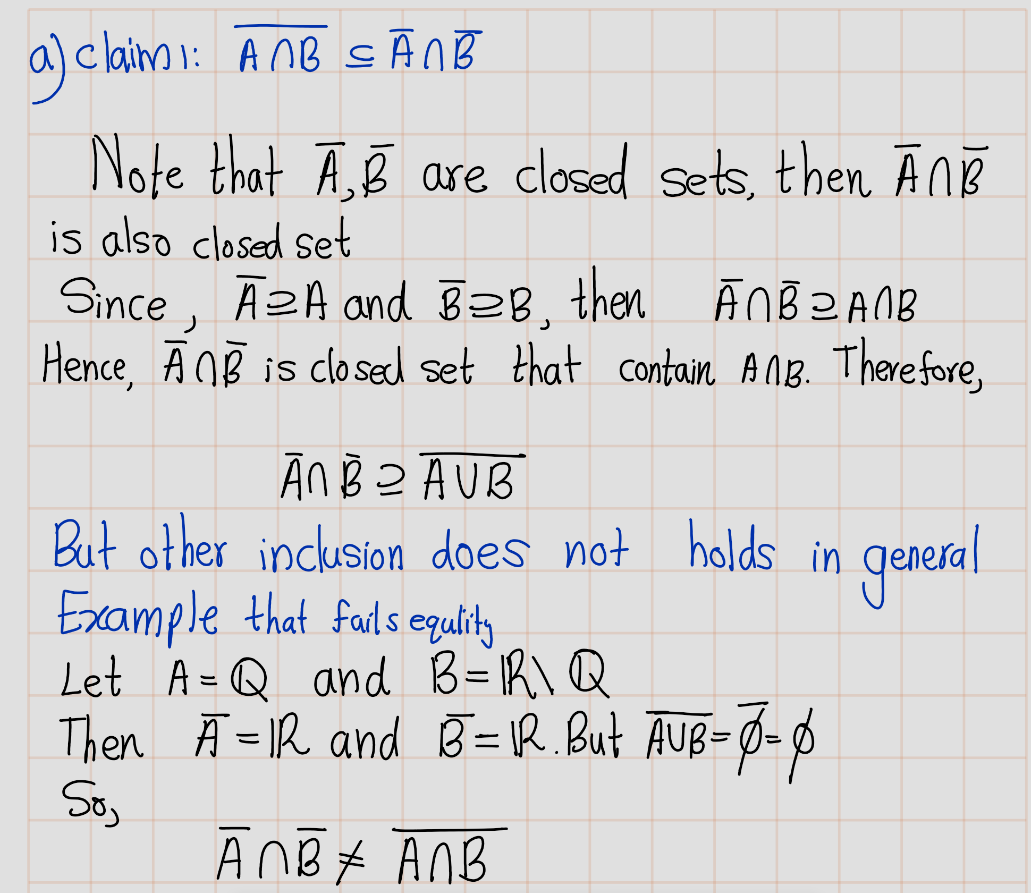
\includegraphics{figures/Exercises/Ex 2.17/ex-8-1.png}

(b)\\
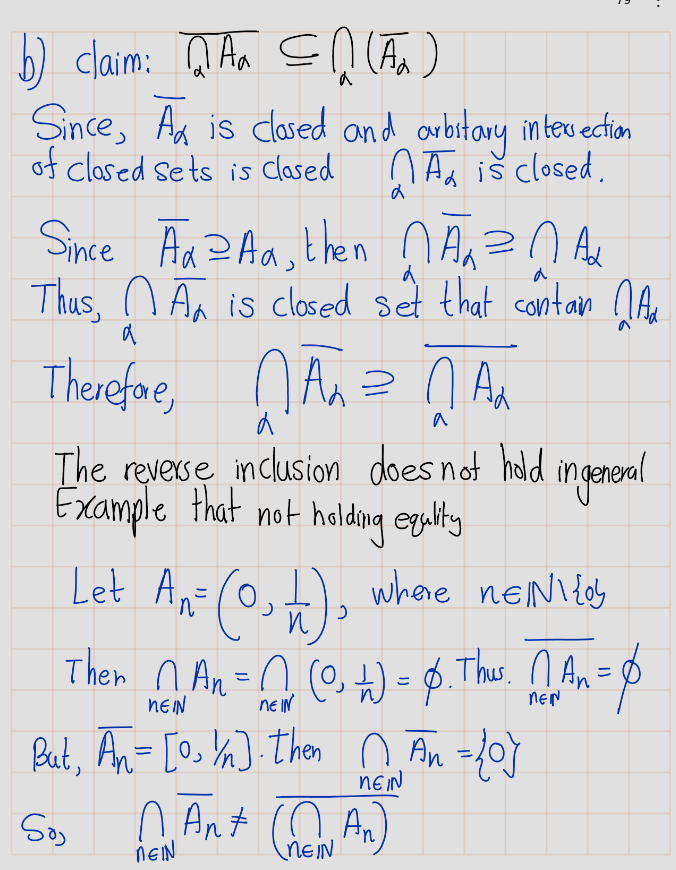
\includegraphics{figures/Exercises/Ex 2.17/ex-8-2.png}

(c)\\
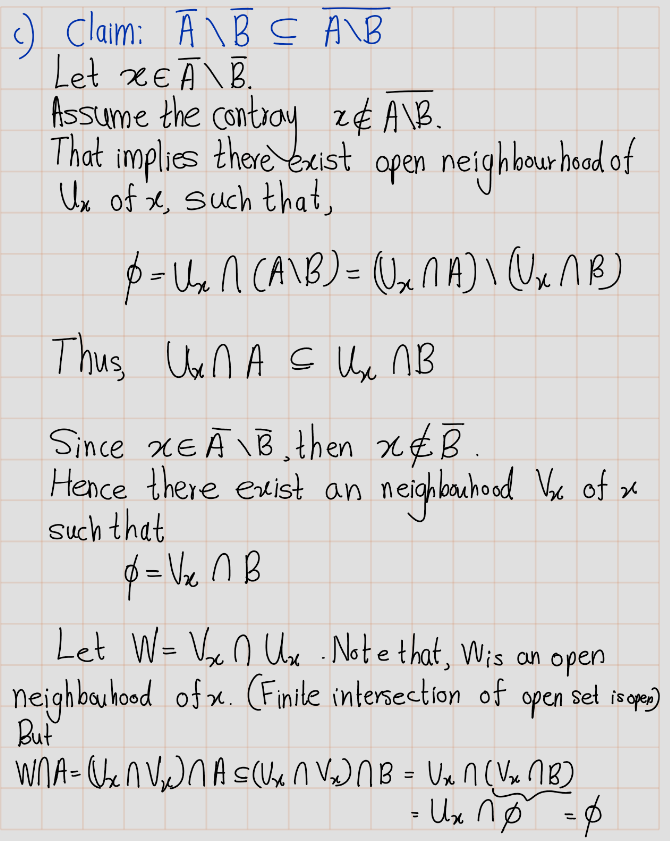
\includegraphics{figures/Exercises/Ex 2.17/ex-8-3.png}
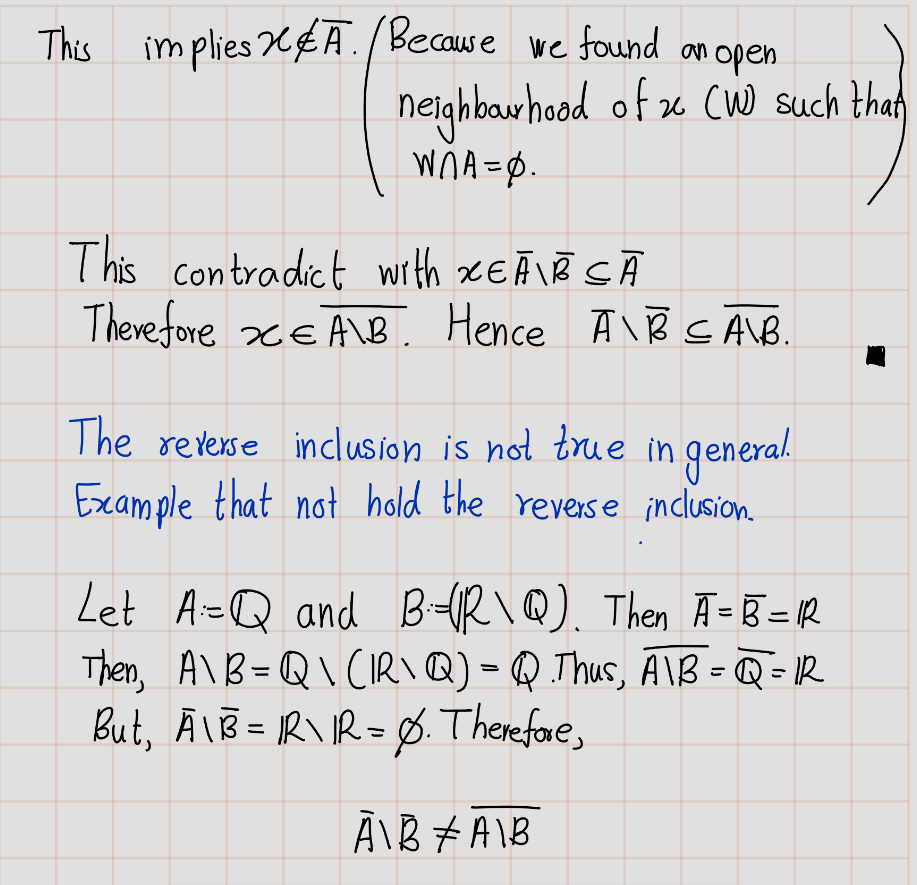
\includegraphics{figures/Exercises/Ex 2.17/ex-8-4.png}

\begin{exercise}[Mun 2.17.9]
\protect\hypertarget{exr:unnamed-chunk-146}{}\label{exr:unnamed-chunk-146}Let \(A \subset X\) and \(B \subset Y\). Show that in the space \(X \times Y\),
\[\overline{A \times B} = \overline{A} \times \overline{B}\].
\end{exercise}

\includegraphics{figures/Exercises/Ex 2.17/ex-9.png}

\begin{exercise}[Mun 2.17.10]
\protect\hypertarget{exr:Hausdorff1}{}\label{exr:Hausdorff1}Show that every order topology is Hausdorff.
\end{exercise}

\includegraphics{figures/Exercises/Ex 2.17/ex-10.png}

\begin{exercise}[Mun 2.17.11]
\protect\hypertarget{exr:Hausdorff2}{}\label{exr:Hausdorff2}Show that the product of two Hausdorff spaces is Hausdorff.
\end{exercise}

\includegraphics{figures/Exercises/Ex 2.17/ex-11.png}

\begin{exercise}[Mun 2.17.12]
\protect\hypertarget{exr:Hausdorff3}{}\label{exr:Hausdorff3}Show that a subspace of a Hausdorff space is Hausdorff.
\end{exercise}

\includegraphics{figures/Exercises/Ex 2.17/ex-12.png}

\begin{exercise}[Mun 2.17.13]
\protect\hypertarget{exr:unnamed-chunk-151}{}\label{exr:unnamed-chunk-151}Show that \(X\) is Hausdorff if and only if the diagonal \(\Delta = \{x\times x | x \in X\}\) is closed in \(X \times X\).
\end{exercise}

\includegraphics{figures/Exercises/Ex 2.17/ex-13.png}

\begin{exercise}[Mun 2.17.14]
\protect\hypertarget{exr:unnamed-chunk-153}{}\label{exr:unnamed-chunk-153}In the finite complement topology on \(\mathbb{R}\), to what point or points does the sequence \(x_n = \frac{1}{n}\) converge?
\end{exercise}

\includegraphics{figures/Exercises/Ex 2.17/ex-14.png}

\begin{exercise}[Mun 2.17.15]
\protect\hypertarget{exr:unnamed-chunk-155}{}\label{exr:unnamed-chunk-155}Show the \(T_1\) axiom is equivalent to the condition that for each pair of points of \(X\), each has a neighborhood not containing the other.
\end{exercise}

\includegraphics{figures/Exercises/Ex 2.17/ex-15-1.png}

\includegraphics{figures/Exercises/Ex 2.17/ex-15-2.png}

\begin{exercise}
\protect\hypertarget{exr:unnamed-chunk-158}{}\label{exr:unnamed-chunk-158}

Consider the following five topologies on \(\mathbb{R}\) given

\begin{eqnarray}
\mathcal{T_1} &:=& \text{the standard topology},\\
\mathcal{T_2} &:=& \text{the topology of  } \mathbb{R}_K ,\\
\mathcal{T_3} &:=& \text{the finite complement topology,}\\
\mathcal{T_4} &:=& \text{the upper limit topology, having all sets $(a, b]$ as basis},\\
\mathcal{T_5} &:=& \text{the topology having all sets $(-\infty, a) = \{x | x < a\}$ as basis.}\\
\end{eqnarray}

\begin{enumerate}
\def\labelenumi{(\alph{enumi})}
\tightlist
\item
  Determine the closure of the set \(K = \left\{1/n | n \in \mathbb{Z}^+\right\}\) under each of these topologies.
\item
  Which of these topologies satisfy the Hausdorff axiom? the \(T_1\) axiom?
\end{enumerate}

\end{exercise}

\includegraphics{figures/Exercises/Ex 2.17/Notsure.png}

As a summary

\begin{longtable}[]{@{}ccccc@{}}
\toprule\noalign{}
Topologies & \(\overline{K}\) & Is \(T_2\) space ? & Is \(T_1\) Space & \\
\midrule\noalign{}
\endhead
\bottomrule\noalign{}
\endlastfoot
\(\mathcal{T_1}\) & \(K\cup\{0\}\) & \(\checkmark\) & \(\times\) & \\
\(\mathcal{T_2}\) & \(K\) & \(\checkmark\) & \(\checkmark\) & \\
\(\mathcal{T_2}\) & \({0}\) & \(\checkmark\) & \(\checkmark\) & \\
\(\mathcal{T_2}\) & \(K\) & \(\checkmark\) & \(\checkmark\) & \\
\(\mathcal{T_2}\) & \([0,\infty)\) & \(\checkmark\) & \(\checkmark\) & \\
\(\mathcal{T_2}\) & \({0}\) & \(\checkmark\) & \(\checkmark\) & \\
\end{longtable}

\begin{exercise}[Mun 2.17.17]
\protect\hypertarget{exr:unnamed-chunk-160}{}\label{exr:unnamed-chunk-160}Consider the lower limit topology on \(\mathbb{R}\) and the topology given by the basis \(C\) of Exercise 8 of §13. Determine the closures of the intervals \(A = (0, \sqrt{2})\) and \(B = (\sqrt{2}, 3)\) in these two topologies.
\end{exercise}

\includegraphics{figures/Exercises/Ex 2.17/Notsure.png}

\begin{exercise}[Mun 2.17.18]
\protect\hypertarget{exr:unnamed-chunk-162}{}\label{exr:unnamed-chunk-162}Determine the closures of the following subsets of the ordered square:
\begin{align}
A &:= \left\{\frac{1}{n} \times 0 \mid n \in \mathbb{Z}^{+}\right\}, \\
B &:= \left\{\left(1 - \frac{1}{n}\right) \times \frac{1}{2} \mid n \in \mathbb{Z}^{+}\right\}, \\
C &:= \left\{x \times 0 \mid 0 < x < 1\right\}, \\
D &:= \left\{x \times \frac{1}{2} \mid 0 < x < 1\right\}, \\
E &:= \left\{\frac{1}{2} \times y \mid 0 < y < 1\right\}.
\end{align}
\end{exercise}

\includegraphics{figures/Exercises/Ex 2.17/ex-18-1.png}
\includegraphics{figures/Exercises/Ex 2.17/ex-18-2.png}
\includegraphics{figures/Exercises/Ex 2.17/ex-18-3.png}

\includegraphics{figures/Exercises/Ex 2.17/ex-18-4.png}

\includegraphics{figures/Exercises/Ex 2.17/ex-18-5.png}

\includegraphics{figures/Exercises/Ex 2.17/ex-18-6.png}

\includegraphics{figures/Exercises/Ex 2.17/ex-18-7.png}

\includegraphics{figures/Exercises/Ex 2.17/ex-18-8.png}

\begin{exercise}[Mun 2.17.19]
\protect\hypertarget{exr:unnamed-chunk-171}{}\label{exr:unnamed-chunk-171}

If \(A \subset X\), we define the boundary of \(A\) by the equation
\[\text{Bd} \, A = \overline{A} \cap \overline{(X \setminus A)}.\]

\begin{enumerate}
\def\labelenumi{(\alph{enumi})}
\tightlist
\item
  Show that \(\text{Int} \, A\) and \(\text{Bd} \, A\) are disjoint, and \(\overline{A} = \text{Int} \, A \cup \text{Bd} \, A\).
\item
  Show that \(\text{Bd} \, A = \emptyset \Leftrightarrow A\) is both open and closed.
\item
  Show that \(U\) is open \(\Leftrightarrow \text{Bd} \, U = \overline{U} \setminus U\).
\item
  If \(U\) is open, is it true that \(U = \text{Int}(\overline{U})\)? Justify your answer.
\end{enumerate}

\end{exercise}

\textbf{Solution}

\begin{enumerate}
\def\labelenumi{(\alph{enumi})}
\tightlist
\item
  Show that \(\text{Int} \, A\) and \(\text{Bd} \, A\) are disjoint, and \(\overline{A} = \text{Int} \, A \cup \text{Bd} \, A\).
\end{enumerate}

\includegraphics{figures/Exercises/Ex 2.17/ex-19-1.png}
\includegraphics{figures/Exercises/Ex 2.17/ex-19-2.png}

\begin{enumerate}
\def\labelenumi{(\alph{enumi})}
\setcounter{enumi}{1}
\tightlist
\item
  Show that \(\text{Bd} \, A = \emptyset \Leftrightarrow A\) is both open and closed.
\end{enumerate}

\includegraphics{figures/Exercises/Ex 2.17/ex-19-3.png}

\includegraphics{figures/Exercises/Ex 2.17/ex-19-4.png}

\begin{enumerate}
\def\labelenumi{(\alph{enumi})}
\setcounter{enumi}{2}
\tightlist
\item
  Show that \(U\) is open \(\Leftrightarrow \text{Bd} \, U = \overline{U} \setminus U\).
\end{enumerate}

\includegraphics{figures/Exercises/Ex 2.17/ex-19-5.png}

d)(d) If \(U\) is open, is it true that \(U = \text{Int}(\overline{U})\)? Justify your answer.

\includegraphics{figures/Exercises/Ex 2.17/ex-19-6.png}

\begin{exercise}[Mun 2.17.20]
\protect\hypertarget{exr:unnamed-chunk-178}{}\label{exr:unnamed-chunk-178}

Find the boundary and the interior of each of the following subsets of \(\mathbb{R}^2\):

\begin{enumerate}
\def\labelenumi{(\alph{enumi})}
\tightlist
\item
  \(A = \{(x, y) | y = 0\}\)
\item
  \(B = \{(x, y) | x > 0 \text{ and } y \neq 0\}\)
\item
  \(C = A \cup B\)
\item
  \(D = \{(x, y) | x \text{ is rational}\}\)
\item
  \(E = \{(x, y) | 0 < x^2 - y^2 \leq 1\}\)
\item
  \(F = \{(x, y) | x \neq 0 \text{ and } y \leq \frac{1}{x}\}\)
\end{enumerate}

\end{exercise}

\textbf{Solution}

\begin{enumerate}
\def\labelenumi{(\alph{enumi})}
\tightlist
\item
  \(A = \{(x, y) | y = 0\}\)
\end{enumerate}

\includegraphics{figures/Exercises/Ex 2.17/ex-20-1.png}

\begin{enumerate}
\def\labelenumi{(\alph{enumi})}
\setcounter{enumi}{1}
\tightlist
\item
  \(B = \{(x, y) | x > 0 \text{ and } y \neq 0\}\)
\end{enumerate}

\includegraphics{figures/Exercises/Ex 2.17/ex-20-2.png}

\begin{enumerate}
\def\labelenumi{(\alph{enumi})}
\setcounter{enumi}{2}
\tightlist
\item
  \(C = A \cup B\)
\item
  \(D = \{(x, y) | x \text{ is rational}\}\)
\item
  \(E = \{(x, y) | 0 < x^2 - y^2 \leq 1\}\)
\item
  \(F = \{(x, y) | x \neq 0 \text{ and } y \leq \frac{1}{x}\}\)
\end{enumerate}

  \bibliography{book.bib,packages.bib}

\end{document}
